\documentclass[11pt,pdftex,]{book}
\setlength{\parskip}{0pt}
% number the lines:

%\fancyfoot[LE,RO]{\thepage}

\newcommand{\setlinenumbers}{false}

% use double spacing:
\newcommand{\setdoublespacing}{false}

% show authors:
\newcommand{\showauthors}{true}

% show keywords:
\newcommand{\showkeywords}{false}

% show author contributions:
\newcommand{\showcontributions}{false}

% figures and captions at end:
\newcommand{\figsatend}{false}

% remove images from figures:
\newcommand{\nofigs}{false}


%%%%%%%%%%%%%%%%%%%%%%%%%%%%%%%%%%%%%%%%%%%%%%%%%%%%%%%%%%%%%%%%%%%%%%%%%%%%%
%%%%% line numbering, spacing, authors, keywords %%%%%%%%%%%%%%%%%%%%%%%%%%%%
\usepackage{ifthen}

\usepackage{wasysym}

\ifthenelse{\boolean{\setlinenumbers}}{%
\usepackage{lineno}\linenumbers}%
{\newenvironment{linenomath}{}{}}

\ifthenelse{\boolean{\setdoublespacing}}{%
\usepackage{setspace}\doublespacing}{}

\ifthenelse{\boolean{\showauthors}}{}{\author{}\date{}}

\usepackage[inline]{enumitem}
\newenvironment{keywords}%
{\paragraph{Keywords}\begin{itemize*}[label={},itemjoin={~$|$\ },afterlabel={}]}%
{\end{itemize*}\par}
\usepackage{comment}
\ifthenelse{\boolean{\showkeywords}}{}{\excludecomment{keywords}}

\newenvironment{contributions}{\section{Author contributions}}{\par}
\ifthenelse{\boolean{\showcontributions}}{}{\excludecomment{contributions}}


%%%%% page style %%%%%%%%%%%%%%%%%%%%%%%%%%%%%%%%%%%%%%%%%%%%%%%%%%%%%%%%%%%%
\usepackage{geometry}
\geometry{
	paper=a4paper, % Change to letterpaper for US letter
	%inner=2.5cm, % Inner margin
	%outer=3.8cm, % Outer margin
	inner=3cm,
	outer=2cm,
	bindingoffset=.5cm, % Binding offset
	top=2.5cm, % Top margin
	bottom=2.5cm, % Bottom margin
	%showframe, % Uncomment to show how the type block is set on the page
}
%\pagestyle{myheadings}
\usepackage{fancyhdr}
\pagestyle{fancy}
\fancyhf{}
\fancyfoot[LE,RO]{\thepage}
\fancyhead[LE]{\leftmark}
\fancyhead[RO]{\rightmark}

%%%%% language %%%%%%%%%%%%%%%%%%%%%%%%%%%%%%%%%%%%%%%%%%%%%%%%%%%%%%%%%%%%%%
\usepackage[english]{babel}
\usepackage[utf8]{inputenc} % Required for inputting international characters

%%%%% fonts %%%%%%%%%%%%%%%%%%%%%%%%%%%%%%%%%%%%%%%%%%%%%%%%%%%%%%%%%%%%%%%%
\usepackage{pslatex}   % nice font for pdf file

%%%%% section style %%%%%%%%%%%%%%%%%%%%%%%%%%%%%%%%%%%%%%%%%%%%%%%%%%%%%%%%%
\usepackage[sf,bf,it,big,clearempty]{titlesec}
\setcounter{secnumdepth}{1}

%%%%% units %%%%%%%%%%%%%%%%%%%%%%%%%%%%%%%%%%%%%%%%%%%%%%%%%%%%%%%%%%%%%%%%%
\usepackage[mediumspace,mediumqspace,Gray]{SIunits}      % \ohm, \micro
\usepackage{textcomp}
%%%%% graphics %%%%%%%%%%%%%%%%%%%%%%%%%%%%%%%%%%%%%%%%%%%%%%%%%%%%%%%%%%%%%%
\usepackage{xcolor}
\usepackage{wrapfig}
%\pagecolor{white}
\usepackage{graphicx}
\usepackage{tabularx}
\newcommand{\trh}{\rule[-1ex]{0pt}{3.5ex}}
\newcommand{\trt}{\rule{0pt}{2.5ex}}

\newcolumntype{L}[1]{>{\raggedright\let\newline\\\arraybackslash\hspace{0pt}}m{#1}}
\newcolumntype{C}[1]{>{\centering\let\newline\\\arraybackslash\hspace{0pt}}m{#1}}
\newcolumntype{R}[1]{>{\raggedleft\let\newline\\\arraybackslash\hspace{0pt}}m{#1}}


% references of equations
\newcommand{\eqnref}[1]{Eq.\,(\ref{#1})}
\newcommand{\eqnrefb}[1]{Eq.\,\ref{#1}}

\usepackage{xr}
\newcommand{\chapref}[1]{Chapter~\ref{#1}}

%%%%% figures %%%%%%%%%%%%%%%%%%%%%%%%%%%%%%%%%%%%%%%%%%%%%%%%%%%%%%%%%%%%%%%

% captions:
\ifthenelse{\boolean{\setdoublespacing}}{%
\usepackage[format=plain,singlelinecheck=off,labelfont=bf,font={small,sf,doublespacing}]{caption}}%
{\usepackage[format=plain,singlelinecheck=off,labelfont=bf,font={small,sf}]{caption}}

% put caption on separate float:
\newcommand{\breakfloat}{\end{figure}\begin{figure}[t]}

% references to panels of a figure within the caption:
\newcommand{\figitem}[1]{\textsf{\bfseries\uppercase{#1}}\penalty10000 }
% references to panels of a figure within the text:
\newcommand{\panel}[1]{\textsf{#1}}
% references to figures:
\newcommand{\fref}[1]{\textup{\ref{#1}}}
\newcommand{\subfref}[2]{\textup{\ref{#1}}\,\panel{#2}}
% references to figures in normal text:
\newcommand{\fig}{Fig.}
\newcommand{\Fig}{Fig.}
\newcommand{\figs}{Figs.}
\newcommand{\Figs}{Figs.}
\newcommand{\figref}[1]{\fig~\fref{#1}}
\newcommand{\Figref}[1]{\Fig~\fref{#1}}
\newcommand{\figsref}[1]{\figs~\fref{#1}}
\newcommand{\Figsref}[1]{\Figs~\fref{#1}}
\newcommand{\subfigref}[2]{\fig~\subfref{#1}{#2}}
\newcommand{\Subfigref}[2]{\Fig~\subfref{#1}{#2}}
\newcommand{\subfigsref}[2]{\figs~\subfref{#1}{#2}}
\newcommand{\Subfigsref}[2]{\Figs~\subfref{#1}{#2}}
% references to figures within brackets:
\newcommand{\figb}{Fig.}
\newcommand{\Figb}{Fig.}
\newcommand{\figsb}{Figs.}
\newcommand{\Figsb}{Figs.}
\newcommand{\figrefb}[1]{\figb~\fref{#1}}
\newcommand{\Figrefb}[1]{\Figb~\fref{#1}}
\newcommand{\figsrefb}[1]{\figsb~\fref{#1}}
\newcommand{\Figsrefb}[1]{\Figsb~\fref{#1}}
\newcommand{\subfigrefb}[2]{\figb~\subfref{#1}{#2}}
\newcommand{\Subfigrefb}[2]{\Figb~\subfref{#1}{#2}}
\newcommand{\subfigsrefb}[2]{\figsb~\subfref{#1}{#2}}
\newcommand{\Subfigsrefb}[2]{\Figsb~\subfref{#1}{#2}}

% figure placement:
\ifthenelse{\boolean{\figsatend}}{%
\setcounter{topnumber}{10}%
\setcounter{totalnumber}{10}%
\renewcommand{\textfraction}{0.0}%
\renewcommand{\topfraction}{1.0}%
\renewcommand{\floatpagefraction}{0.0}%
\usepackage[nolists,markers,figuresonly]{endfloat}%
\ifthenelse{\boolean{\nofigs}}{\renewcommand{\efloatseparator}{\mbox{}}}{}%
\newcommand{\figurecaptions}{\pagestyle{empty}\clearpage\processdelayedfloats\renewcommand{\figureplace}{}}}%
{\setcounter{topnumber}{1}%
\setcounter{totalnumber}{2}%
\renewcommand{\textfraction}{0.2}%
\renewcommand{\topfraction}{0.8}%
\renewcommand{\floatpagefraction}{0.7}%
\newcommand{\figurecaptions}{}%
}
\newcommand*{\captionc}[1]{\captionof{figure}{#1}}

% no images in figures:
\ifthenelse{\boolean{\nofigs}}{%
\newcommand{\showfigure}[1]{}}%
{\newcommand{\showfigure}[1]{#1}}


% bibliography ----------------------------------
%\usepackage[round,colon]{natbib}

%\usepackage[sectionbib]{natbib}
%\usepackage{chapterbib}
%\renewcommand{\bibsection}{\section{References}}
%\setlength{\bibsep}{2pt}
%\setlength{\bibhang}{1.5em}
%\bibliographystyle{jneurosci}

\usepackage[round,colon]{natbib}
%\renewcommand{\bibsection}{\section*{References}}
\renewcommand{\bibsection}{{\Huge\textbf{Bibliography}}\vspace{2cm}}
\setlength{\bibsep}{8pt}
\setlength{\bibhang}{1.5em}
\bibliographystyle{jneurosci}
 
%\usepackage[breaklinks=true,colorlinks=true,citecolor=blue!30!black,urlcolor=blue!30!black,linkcolor=blue!30!black]{hyperref}
\usepackage[breaklinks=true,colorlinks=true,citecolor=black,urlcolor=black,linkcolor=black]{hyperref}

% chapter format --------------------------------
%\usepackage{titlesec}
%
%\titleformat{\chapter}[display]
%  {  \normalfont\huge\bfseries\centering}{\centering\chaptertitlename\ \thechapter}{20pt}{\Huge}
%\titlespacing*{\chapter} 
%  {0pt}{50pt}{40pt}

% notes -----------------------------------------
\newcommand{\note}[2][]{\textcolor{red!80!black}{[\textbf{\ifthenelse{\equal{#1}{}}{}{#1: }}#2]}}
\newcommand{\notejb}[1]{\note[JB]{#1}}
\newcommand{\notetr}[1]{\note[TR]{#1}}

% -----------------------------------------------
\hyphenation{mo-ni-to-ring mo-da-li-ties court-ship}

% fish species %%%%%%%%%%%%%%%%%%%%%%%%%%%%%%%%%%%%%%%%%%%%%%%%%%%%%%%%%%
\newcommand{\aptero}{\textit{Apteronotus}}
\newcommand{\Albi}{\textit{Apteronotus albifrons}}
\newcommand{\albi}{\textit{A. albifrons}}
\newcommand{\Lepto}{\textit{Apteronotus leptorhynchus}}
\newcommand{\lepto}{\textit{A. leptorhynchus}}
\newcommand{\Rostratus}{\textit{Apteronotus rostratus}}
\newcommand{\rostratus}{\textit{A. rostratus}}
\newcommand{\Macros}{\textit{Apteronotus macrostomus}}
\newcommand{\macros}{\textit{A. macrostomus}}
\newcommand{\Eig}{\textit{Eigenmannia virescens}}
\newcommand{\Eigenmannia}{\textit{Eigenmannia}}
\newcommand{\eig}{\textit{E. virescens}}
\newcommand{\sterno}{\textit{Sternopygus}}

\graphicspath{{figures/}}

%%%%%%%%%%%%%%%%%%%%%%%%%%%%%%%%%%%%%%%%%%%%%%%%%%%%%%%%%%%%%%%%%%%%%%%%%%%
%%%%%%%%%%%%%%%%%%%%%%%%%%%%%%%%%%%%%%%%%%%%%%%%%%%%%%%%%%%%%%%%%%%%%%%%%%%
\begin{document}
%\newpage

%\maketitle

\begin{titlepage}
\begin{center}

\vspace*{.06\textheight}
%{\scshape\LARGE Eberhard Karls Universität Tübingen\par}\vspace{1.5cm} % University name
%\textsc{\Large Doctoral Thesis}\\[0.5cm] % Thesis type
% \hrule\vspace{0.4cm} % Horizontal line

{\huge \bfseries Social structures and interactions in electric fish explored by large-scale signal tracking
\par}\vspace{0.4cm} 

% adaptive, probabilistic, 

%Exploration of social structures and interactions by means of custom signal tracking\\in an electric fish

% Thesis title
% \hrule % Horizontal line
\vfill
\vspace{3cm}
{\Large \textbf{Dissertation}\\
der Mathematisch-Naturwissenschaftlichen Fakultät\\
der Eberhard Karls Universität Tübingen\\
zur Erlangung des Grades eines\\
Doktors der Naturwissenschaften\\
(Dr. rer. nat.)\\}
\vspace{3.5cm}
{\Large vorgelegt von\\Till Raab\\aus Tübingen\\}
\vspace{4cm}
{\Large Tübingen\\\vspace{0.1cm}
2021}\\[4cm] % Date
%\includegraphics{Logo} % University/department logo - uncomment to place it
 
\vfill
\end{center}
\end{titlepage}

%%%%%%%%%%%%%%%%%%%%%%%%%%%%%%%%%%%%%%%%%%%%%%%%%%%%%%%%%%%%%%%%%%%%%%%%%%%
\thispagestyle{empty}
\vspace*{\fill}

\noindent
{\large Gedruckt mit Genehmigung der Mathematisch-Naturwissenschaftlichen Fakultät der\\
Eberhard Karls Universität Tübingen.\\}
\vspace{1cm}

\hspace{-0.7cm}
\noindent
\begin{minipage}{0.49\textwidth}
{\large Tag der mündlichen Qualifikation:\\
Dekan:\\
1. Berichterstatter/-in:\\
2. Berichterstatter/-in:\\}
\end{minipage}\hfill
\begin{minipage}{0.49\textwidth}
\noindent
{\large 24.03.2022\\
Prof. Dr. Thilo Stehle\\
Prof. Dr. Jan Benda\\
Prof. Dr. Steffen Hage\\}
\end{minipage}
\clearpage
%%%%%%%%%%%%%%%%%%%%%%%%%%%%%%%%%%%%%%%%%%%%%%%%%%%%%%%%%%%%%%%%%%%%%%%%%%%

\pagenumbering{Roman}
\setcounter{tocdepth}{1}
\vspace{-2cm}
{
  \hypersetup{linkcolor=black}
  \tableofcontents
}
%\tableofcontents
\addtocontents{toc}{\protect\enlargethispage{\baselineskip}}

\chapter*{Abstract}
\addcontentsline{toc}{chapter}{Abstract}

In order to persist under the pressure of natural selection, organisms need to adapt to the multiple aspects of their surrounding environment. As a result, various forms of social organizations developed across animal species. Living in groups can be beneficial since it allows animals to cooperate in tasks of their everyday lives. However, intraspecific competitions for limited resources and associated costs are increased in groups. Accordingly, animals developed numerous strategies and social behaviors in order to economize competitions. For weakly electric fish, knowledge about such natural, social behaviors is scarce since conclusive behavioral observations are limited by their nocturnal and secretive lifestyle. Yet their unique electric signals, produced by discharges of an electric organ (EOD), provide an excellent opportunity to monitor individual behaviors in freely moving and interacting populations. The EODs of whole groups can be recorded with recording electrode arrays submerged in the water and then be tracked for individual fish by means of various signal features.

In \chapref{Methods}, we present a semi-automatic system capable of tracking electric signals of wave-type electric fish with unprecedented accuracy. Our algorithm benefits from combining and refining previous approaches of tracking individual specific EOD frequencies (EODf) and spatial electric field properties. In this process, the similarity of signal pairs in discrete data windows determines their tracking order. With our advancements, we are capable of resolving most algorithmic issues that occur while tracking individual electric signals in freely behaving groups of wave-type electric fish.

On the basis of tracked EOD traces, we characterized individual spatial-temporal behaviors within a group of 14 brown ghost knifefish, \Lepto{}, over 10 consecutive days (\chapref{Habitats}). In this experiment, fish have been housed in a large communal tank stocked with several naturalistic habitats. The evaluated movement patterns suggest fish to mainly distribute independently from each other according to the presence of suitable shelters. Males with higher EODf showed enhanced explorative behavior during the night and increased territoriality during the day. Both could represent manifestations or displays of dominance, supporting the hypothesis of EODf indicating social status in males. In females, higher EODf seems to indicate more active character traits since movement activities during both day and night increased with EODf.

In order to determine how \lepto{} resolves conflicts, we evaluated behaviors and interactions of unfamiliar pairs of \lepto{} during staged competitions (\chapref{Competitions}). Winners were primarily determined by a larger body size. During competitions, losers continuously emitted rises as electrocommunication signals. These signals frequently provoked ritualized fighting and chase behaviors by the other fish. The number of rises emitted by losers and the duration of chase behaviors depended in similar ways on the contestants' physical attributes. Detailed evaluations of these correlations suggest \lepto{} to adjust their competition behavior according to mutual assessment, whereby rises could signal a loser's motivation to continue assessment through ritualized fighting.

Based on our observations, we suggest \lepto{} to actually prefer remaining solitary. Nevertheless, frequent interactions and conflicts with conspecifics are inevitable because of their abundance. In order to resolve these conflicts economically, \lepto{} establishes a dominance hierarchy. The interplay of rises and agonistic attacks in associated competitions could be used to adjust the skewness in access to resources across social ranks. Males seem to be more motivated to compete and attain higher social ranks, whereas females seem to limit their active participation in dominance fights to occasions where resources are rather scarce, like in our competition experiments. 

\makeatletter
\@openrightfalse
\makeatother
\chapter*{Deutschsprachige Zusammenfassung}
\addcontentsline{toc}{chapter}{Deutschsprachige Zusammenfassung}

%Alle Organismen, die sich im Verlauf der Evolutionsgeschichte über die Jahrmillionen entwickelt haben, haben sich durch Adaptation an die Bedingungen ihrer Lebensräume angepasst.

Im Verlauf der Evolutionsgeschichte haben sich über die Jahrmillionen verschiedenste Organismen entwickelt, die sich alle durch Adaptation an die Bedingungen ihrer Lebensräume angepasst haben. Dieser Prozess brachte neben anderen Entwicklungen diverse Sozialformen hervor. Für viele Tierarten erwies sich vor allem das Zusammenleben in Gruppen als vorteilhaft, da dieses vielfältige Möglichkeiten zur Kooperation bietet. Gleichzeitig bedeutet das Leben in einer Gruppe jedoch auch vermehrte Konkurrenz um limitierte Ressourcen. Um diese Konflikte möglichst ökonomisch zu gestalten, haben sich im Tierreich zahlreiche verschiedene soziale Strategien und Verhaltensweisen entwickelt. Bei schwach elektrischen Fischen sind solche Verhaltensweisen bislang nur wenig untersucht, da die Durchführung natürlicher Verhaltensstudien an diesen Tieren durch ihre nachtaktive und zurückgezogene Lebensweise stark erschwert wird. Allerdings eröffnen die charakteristischen elektrischen Signale dieser Fische eine nicht-invasive Möglichkeit, Verhaltensweisen dieser Tiere in sich frei bewegenden und interagierenden Populationen zu erforschen. Die elektrischen Signale ganzer Gruppen von elektrischen Fischen können mithilfe von Elektroden-Gittern im Wasser aufgezeichnet und anhand verschiedener Signalparameter für individuelle Tiere getrackt werden.

In Kapitel~\ref{Methods} wird ein eigens entwickelter Algorithmus vorgestellt, welcher mit bis dahin unerreichter Genauigkeit ermöglicht, die elektrischen Signale einzelner Fische anhand der individuell spezifischen Entladungsfrequenz ihrer elektrischen Organe (EOD) und der räumlichen Ausdehnung der daraus resultierenden elektrischen Felder zu tracken. Anhand dieser beiden Signalparameter kann die Ähnlichkeit von Signalpaaren quantifiziert werden. Dies ermöglicht, Signalpaare in einer Reihenfolge von absteigender Ähnlichkeit zu verbinden, um dadurch individuelle Signalspuren einzelner Tiere zu erhalten. Um die benötigte Rechenkapazität für ein solches Tracking-Verfahren zu begrenzen, werden zunächst Signalpaare in sich überlappenden 30\,Sekunden ``tracking windows'' gebildet. In einem darauffolgenden Schritt werden die daraus gewonnenen Signalspuren miteinander verbunden. Durch diesen neuen Algorithmus, welcher vorangegangene Ansätze kombiniert und weiterentwickelt, können die meisten auftretenden Tracking-Probleme gelöst werden, die sich bei der Analyse elektrischer Signale von sich frei bewegenden elektrischen Fischen ergeben. 

Anhand getracker EOD Spuren wurden im Labor die Bewegungsmuster von 14 braunen Messerfischen, \Lepto{}, über einen Zeitraum von 10 aufeinanderfolgenden Tagen hinweg rekonstruiert und charakterisiert (Kapitel~\ref{Habitats}). Besagtes Experiment wurde in einem 2\,m$^3$ großen Aquarium durchgeführt, in dem sich die Fische frei zwischen mehreren natürlichen Habitaten bewegen konnten. Die Fische schienen sich unabhängig voneinander entsprechend der Verfügbarkeit geeigneter Unterschlüpfe im Aquarium zu verteilen. Männchen mit höherer EOD Frequenz zeigten erhöhte Bewegungsaktivität bzw. Explorationsverhalten in der Nacht und verhielten sich stationärer während des Tages. Da solche Verhaltensmuster als Charakteristika oder als Demonstrationen von Dominanz interpretiert werden können, unterstützen diese Beobachtungen die Hypothese, dass die EOD Frequenz männlicher \lepto{} auf ihren sozialen Status schließen lässt. Bei Weibchen hingegen scheinen höhere EOD Frequenzen auf generell aktivere Wesenszüge hinzudeuten, da Weib-chen mit höheren EOD Frequenzen sowohl bei Tag als auch bei Nacht erhöhte Bewegungsaktivität zeigten.

In einem weiteren Experiment, in dem \lepto{} paarweise um einen qualitativ hochwertigen Unterschlupf konkurrierten, wurde untersucht, wie \lepto{} Konflikte löst und welche Verhaltensweisen dabei angewendet werden (Kapitel~\ref{Competitions}). In den meisten Versuchsdurchläufen besetzte das größere Tier am Ende des Versuchs den hochwertigen Unterschlupf und wurde so als Gewinner identifiziert. Während der Versuche interagierten die Fische durch ritualisiertes Kampfverhalten und Elektrokommunikation. Die unterlegenen Fische produzierten dabei kontinuierlich sogenannte ``Rises'', obwohl daraufhin der überlegene Fisch häufiger agonistische Interaktionen initiierte. Die Anzahl der detektierten ``Rises'' und die Dauer von agonistischen Interaktionen konnte gleichermaßen mit den physischen Eigenschaften beider Fische in Verbindung gebracht werden. Die detaillierte Analyse dieser Zusammenhänge deutet darauf hin, dass \lepto{} die Kampfkraft eines Gegners anhand von verschiedenen aktiven und passiven Signalen sowie ritualisiertem Kampfverhalten abschätzt, mit der eigenen Kampfkraft vergleicht und sein Verhalten entsprechend des Unterschiedes anpasst. Dabei könnten Rises von unterlegenen Tieren dazu genutzt werden, ihre Motivation zur Fortführung ritualisierter Kämpfe zu signalisieren.

Die in der vorliegenden Dissertation beschriebenen Verhaltensstudien deuten darauf hin, dass \lepto{} eigentlich eine Lebensweise als Einzelgänger gegenüber dem Zusammenleben in Gruppen bevorzugt. Allerdings sind regelmäßige Interaktionen und Rivalitäten mit Artgenossen durch ihre weite und dichte Verbreitung unumgänglich. Um die aus repetitiven Kämpfen entstehenden hohen Kosten zu verringern, etabliert \lepto{} eine soziale Hierarchie. In den zum Zwecke dieser Hierarchiebildung stattfindenden ritualisierten Kämpfen könnte das Zusammenspiel von ``Rises'' und agonistischen Interaktionen den Dominanzunterschied und damit die Verteilung von Ressourcen zwischen den Tieren definieren. Weiterhin lassen Verhaltensunterschiede zwischen Männchen und Weibchen annehmen, dass der Ausgang von Rivalitätskämpfen und der individuelle soziale Status für Männchen wichtiger sind als für Weibchen. Letztere scheinen ihre aktive Teilnahme an Dominanzkämpfen auf Situationen zu beschränken, in welchen Ressourcen stark limitiert sind.


\thispagestyle{plain}

%\chapter*{Deutschsprachige Zusammenfassung}
%\addcontentsline{toc}{chapter}{Deutschsprachige Zusammenfassung}
%
%Alle Organismen, die sich im Verlauf der Evolutionsgeschichte über die Jahrmillionen entwickelten, haben sich durch Adaptation an die Bedingungen ihrer Lebensräume angepasst. Dieser Prozess brachte neben anderen Entwicklungen die verschiedensten Sozialformen hervor. Für viele Tierarten erwies sich das Zusammenleben in Gruppen als vorteilhaft. Ein zentraler Faktor sind dabei die vielfältigen Möglichkeiten zur kooperation bezüflich der Anforderungen des täglichen Überlebens.
%
%In Gruppen profitieren Tiere von den vielfältigen Möglicheiten zur Kooperation. Allerdings bedeutet das Leben in einer Gruppe auch vermehrte Konkurenz um limiterte Resourcen. Um diese Konflike möglichst ökonomisch zu gestalten haben sich im Tierreich verschiedene Verhaltensweisen und Konfliktlösungsstrategien entwickelt. 
%
%Solche Verhaltensweisen sind in schwach elektrischen Fischen bislang wenig untersucht, da die Möglichkeiten for natürliche Verhaltensstudien an diesen Tieren durch ihre nachtaktiven und zurückgezogenen Lebensweisen stark limitiert sind. Allerdings eröffnet sich durch die eigens erzeugten elektrischen Signale dieser Fische eine nicht-invasive Möglichkeit Verhaltesweisen einzelner Tiere in sich frei bewegenden und interagierenden Pupulationen zu untersuchen. Die elektrischen Signale von elektrischen Fischen können mithilfe von Elektroden-Gittern im Wasser aufgezeichnet und anhand verschiedener Signalparameter für individuelle Tiere getrackt werden.
%
%In Kapitel~\ref{Methods} wird ein Algorithmus vorgestellt, der ermöglicht die elektrischen Signale einzelner Fische anhand der individuell speziefischen Entladungsfrequenz ihrer eketrischen Organe (EOD) und der räumlichen Ausdehnung der daraus resultierenden eketrischen Felder zu tracken. Durch diese Signalparameter kann die Ähnlichkeit von Signalpaaren quantifiziert werden. Dies ermöglicht Signalpaare in einer Reihenfolge von absteigender Ähnlichkeit zu verbinden um dadurch individualle Signalspuren eizelner Tiert zu erhalten. Um die benötigte Rechenkapazität für ein solches Tracking in Grenzen zu halten werden zunächst Signalpaare in sich überlappenden 30\,Sekunden ``tracking windows'' gebildet. In einem darauffolgenden Schritt werden die daraus resultierenden Signalspuren verbunden. In dem vorgestellen Algorithmus wurden Ideen früherer Tracking-Ansätze kombiniert und weiterentwickelt. Dadurch können die meisten schwierigen Tracking Probleme, welche sich bei der Analyse von eletrischen Signalen sich frei bewegender elektrischer Fische ergeben, gelöst werden. 
%
%Anhand getracker EOD Spuren konnten im Labor die Bewegungsmuster von 14 braunen Messerfischen, \Lepto{}, rekonstruiert und charakterisiert werden (Kapitel~\ref{Habitats}). Besagtes Experiment wurde in einem großen Aquarium durchgeführt, in dem sich die Fische frei zwischen mehreren natürlichen Habitaten bewegen konnten. Die Fische schienen sich unabhängig voneinander, entsprechend der Verfügbarkeit von geeigneten Unterschlüpfen im Aquarium zu verteilen. Männchen mit höherer EOD Frequenz zeigen erhörte Bewegungsaktivität/Explorationsverhalten in der Nacht und waren stationärer währen des Tages. Da solche Verhaltensmuster als Charakteristika oder zur Zurschaustellungen von Dominanz interpretiert werden können unterstützen diese Beobachtungen die Hypothese, dass in männlichen \lepto{} die EOD Frequenz auf den sozialen Status eines Tieres hinweist. Bei Weibchen scheinen höhere EOD Frequenzen auf generell aktivere Persönlichkeiten hinzudeuten, da Weibchen mit höheren EOD Frequenzen sowohl bei Tag als auch bei Nacht erhöhte Bewegungsaktivität zeigten.
%
%In einem weiteren Experiment, in dem \lepto{} paarweise um einen qualitativ hochwertigen Unterschlupf konkurrierten, sollte untersucht werden, wie \lepto{} Konflikte löst und welche Verhaltensweisen dabei vonnöten sind (Kaptile~\ref{Competitions}). In den meisten Versuchsdurchläufen gewann das größere Tier einer Paarung und besetzte am Ende des Versuchs den hochwertigen Unterschlupf. Die Interaktionen der Tiere beinhalteten Elektrokommunikation und ritualisierte Kämpfe. Die Fische, die später als unterlegen identifiziert wurden produzierten während des Versuchs kontinuiertlich so genannte ``Rises'', obwohl der entsprechend überlegene Fisch daraufhin öffters agonisitische Interaktionen initiierte. Die Anzahl der detektierten ``Rises'' und die Dauer von agonistischen Interaktionen konnte mit den physischen Eigenschaften beider Fische in Verbindung gebracht werden. Die detailierten Analyse dieser Zusammenhänge deutet darauf hin, dass \lepto{} die Kampfkraft eines Gegners anhand von verschiedenen aktiven und passiven Signalen sowie ritualisiertem Kampfverhalten abschätzt, mit der eigenen Krampfkraft vergleicht und sein Verhalten entsprechend des Unterschiedes anpasst. Unterlegene Tiere könnten mit Rises ihre Motivation signalisieren ritualisierte Kämpfe fortzuführen, um eine genauere Einschätzung des Kampfkraft Unterschieds zu ihrem Gegner zu bekommen und potentielle sekundäre Nutzen daraus zu ziehen.
%
%Die Verhaltensweisen die im Zuge dieser Dissertation beobachtet und analysiert wurden suggerieren, dass \lepto{} eher ein Einzelgänge ist. Allerdings sind regelmäßige Interaktionen und Rivalitäten mit Artgenossen durch ihre weite und dichte Verbreitung unumgänglich.  Um die hohen Kosten repetitiver Kämpfe zu vermeiden etabliert \lepto{} eine soziale Hierarchie. In zu diesem Zwecke stattfindenden ritualisierten Kämpfen könnte das Zusammenspiel von ``Rises'' und agonistischen Interaktionen die Verteilung von Resourcen zwischen den Tieren definieren. Verhatensunterschieden zwischen Männchen und Weibchen suggerieren, dass der Ausgang von Rivalitätskämpfen und der individuelle sozialer Status für Männchen wichtiger ist als für Weibchen. Letztere könnten ihre aktive Teilnahme an Dominanzkämpfen auf Situationen beschränken, in denen Resources stark limitiert sind.
%\thispagestyle{plain}

%
\cleardoublepage
\chapter*{Acknowledgements}
\addcontentsline{toc}{chapter}{\textbf{Acknowledgements}}

First of all, I would like to thank my supervisor, Jan Benda, for his great support, advice, and companionship throughout all stages of my thesis. Especially the vast amount of freedom he gave to me enabled me to shape the path of my scientific work according to my own interests with only little limitations. I am very grateful for his trust and encouragement and everything we have been able to experience together throughout the last years. I very much enjoyed our inspiring (and sometimes heated) disputes and the many opportunities in which I could learn from and together with him. Many thanks also go to the people I had the pleasure to work with, including my colleagues in the lab, my collaborators, everyone who ensured the success of our fieldtrips to South America, and many more. I received great support and advice from everyone I worked with, and the familiar working atmosphere we all together created was invaluable for the success of my thesis.
\\\\I also want to thank my family and friends who always encouraged and supported me. Especially during the sometimes challenging moments of my thesis they provided compensation and gave me strength. But most of all, I want to thank my wife Lara. She not only supported and encouraged me continuously throughout all these years, but also challenged and inspired me in amazing scientific disputes. She gave invaluable input, questioned my theories and approaches, and helped me to specify and structure my thoughts, which repeatedly led to adjustments and improvements of my scientific work.
\\\\ Finally, I want to thank the Center of Integrative Neuroscience that supported the first three and a half years of my studies with a fellowship.


\cleardoublepage
\pagenumbering{arabic}
\setcounter{page}{1}
\graphicspath{{chapter_1_intro/figures/}}
% crossref 
%\externaldocument{../chapter_2_methods/chapter_methods}
%\externaldocument{../chapter_3_habitats/chapter_habitats}
%\externaldocument{../chapter_4_competition/chapter_competition}

\chapter{Introduction}
\label{Intro}

\section{Social organization across animal species}

The manifold of species, lifestyles, and inhabited ecological nieces that can be found across animal taxa still remains astonishing to scientists and non-scientists alike, even more than a century after Charles Darwin first introduced the concept of evolutionary adaptation. In order to persist under the pressure of natural selection, organisms need to adapt to the different aspects of their environments. With this adaptational process, different forms of social organizations developed across animal species, ranging from animals that stay solitary for most of their life \citep{Cigliano1993, Cornhill2020} to aggregations of several hundreds of individuals, e.g. in large herds of caribous or flocks of birds \citep{Nagy2010, Torney2018}. 

Living in groups can be beneficial, e.g. by means of increasing individual survival chances or reproductive success \citep{Clutton-Brock1999, Sword2005, Bilde2007}. Primarily, this results from the manifold of opportunities to cooperate, e.g. joint territorial and resource defense \citep{Geffen1996, Markham2017}, joint foraging \citep{Hojesjo1998}, shared vigilance and collaborative anti-predator defense \citep{Chivers1995, Clutton-Brock1999, Barber2000, Hass2002, Sword2005}, offspring rearing \citep{DeWoody2000}, etc. On the other hand, groups are more likely to be detected by predators \citep{Cote1995}, their energy expense devoted to foraging is increased \citep{Korstjens2006}, and pathogen and parasite transfer is facilitated \citep{Chapman1995, Cote1995}. Furthermore, individuals in groups also face increased intra-specific competition for limited resources, like food, shelter, or mating partners (e.g. \citealp{Cluttonbrock1979, Janson1985}). The optimal group size for a specific population balances costs and benefits arising from the different aspects of group living. However, these costs and benefits are often distributed unequally, favoring those of higher social status (e.g. \citealp{Janson1985, Wauters1992, Kappeler2008}). Accordingly, rivalries and conflicts between group members are inevitable, wherefore animals developed various mechanisms to economize corresponding social interactions.

\section{Competition and opponent assessment}

Especially in group living species, individuals frequently rival for different limited resources whereby fighting is a key behavior to secure access \citep{Cluttonbrock1979, Chapman1995, Markham2015}. However, competition is costly in terms of energy and time allocated to it as well as an increased risk of injury or death (e.g. \citealp{Briffa2004}). Therefore, individual behavioral decisions during contests are strongly dependent on the associated potential costs and benefits \citep{ArnottElwood2008, ArnottElwood2009}. Often, the best predictor for the outcome of competitions is the contestants' fighting ability, also called resource holding potential (RHP, \citealp{Parker1974}). Usually, larger and stronger individuals win contests since their physical advantages (i.e. higher RHP) directly reflect their increased endurance and potential to inflict damage \citep{Archer1988}. However, additional factors like weaponry, experience, sex, or positional advantages may influence an individual's RHP (reviewed in \citealp{ArnottElwood2008}). 

\begin{figure}[h!]
  \centerline{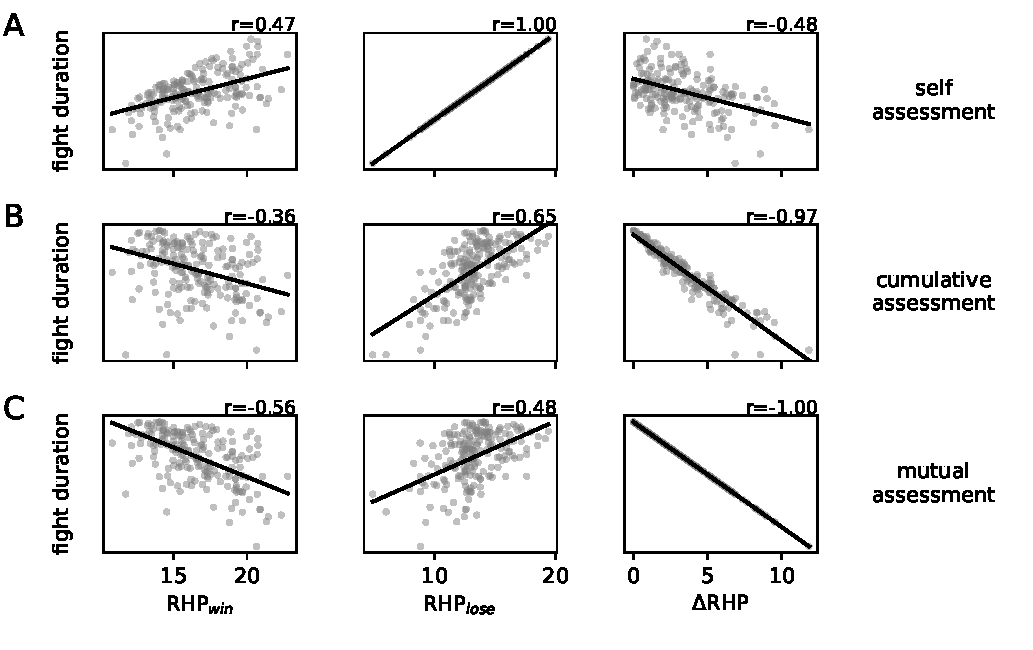
\includegraphics[width=.9\textwidth]{assessment_models_correlations}}
  \caption{\label{assessment_correlations} Dependency of fight duration on the contestants' RHPs and RHP difference ($\Delta$RHP) for different assessment models. Simulations contain competitions between all possible pairings in a population of 1000 individuals with gaussian distributed RHP ($\text{mean}=15$, $\sigma = 3$, only 0.5\,\% shown). P-values of pearson rank correlations were all p$<$0.001. Black lines are linear regressions. For all simulations, costs per second resulting from own actions during competitions ($c_o$) are set to 1\,\textperthousand\, of the mean RHP of the simulated population consistently for all individuals. The amount of damage inflicted by individuals per second ($c_i$) is set to 2\,\% of their own RHP. \figitem{A} Even though the RHP of only the weaker individual (RHP$_{lose}$) is regarded in pure self-assessment (\eqnrefb{self_assessment}), secondary effects, resulting from individuals with higher RHP winning competitions, additionally lead to a positive correlation between fight duration and RHP$_{win}$ and a negative correlation with $\Delta$RHP respectively. Fight duration increases with RHP$_{lose}$ as expected. \figitem{B, C} In contrast, RHPs of both contestants are regarded in cumulative assessment (panel~\panel{B}, \eqnrefb{cum_assessment}) and mutual assessment (panel~\panel{C}, \eqnrefb{mutual_assessment}). In both cases, fight duration increases with RHP$_{lose}$ and decreases with RHP$_{win}$ and $\Delta$RHP, complicating their differentiation. For simulated competitions assuming mutual assessment, fight duration is assumed to linearly increase with increasing $\Delta$RHP, i.e. in \eqnrefb{mutual_assessment}, the exponent $\alpha$ describing the link between $\Delta$RHP and fight duration equals 1.}
\end{figure}

\begin{figure}[t]
  \begin{minipage}[t]{0.66\textwidth}
    \mbox{}\\
    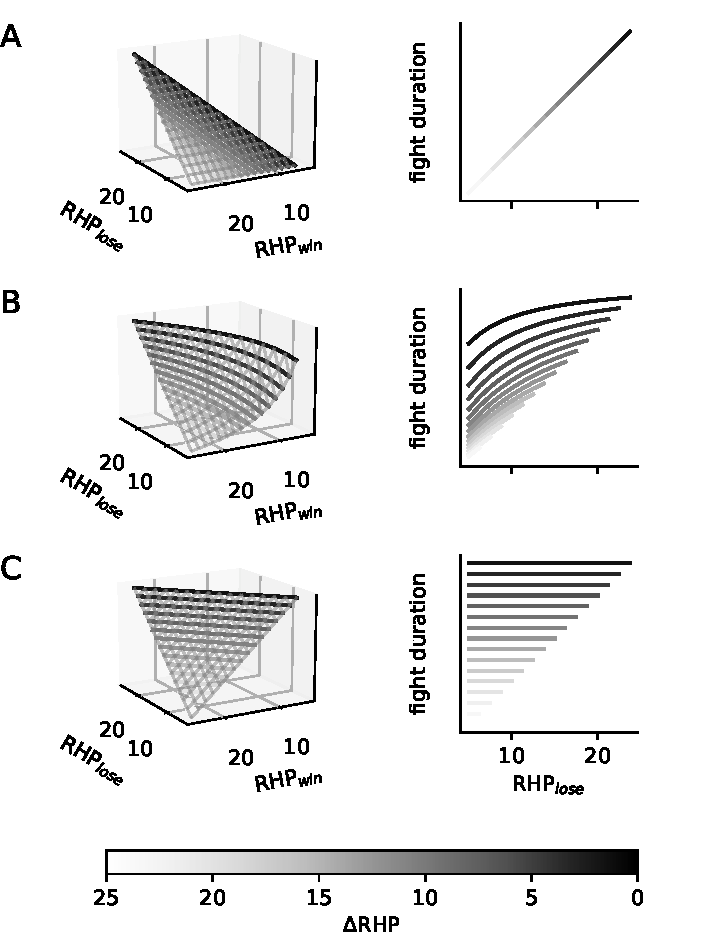
\includegraphics[width=1\textwidth]{assessment_model_simulation}
  \end{minipage}\hfill
  \begin{minipage}[t]{0.3\textwidth}
    \caption{\label{assessment_sim} At fixed RHP differences ($\Delta$RHP), the relation between fight duration and a contestant's RHP varies across assessment models. Panels on the left show how both RHP$_{win}$ and RHP$_{lose}$ influence contest duration ($\Delta t$, z-axis) across the different assessment models, i.e. the basis for simulations shown in \figref{assessment_correlations}. Right panels display the correlation of contest duration and RHP$_{lose}$ for fixed $\Delta$RHP values (grey scale). \figitem{A} In pure self-assessment, the correlation of fight duration and RHP is unaffected by $\Delta$RHP. \figitem{B} In cumulative assessment, fight duration increases with RHP for defined $\Delta$RHPs. \figitem{C} In mutual assessment, fight duration remains unaffected by the contestants' RHP at fixed $\Delta$RHP.}
  \end{minipage}
\end{figure}

The course of competition and associated behaviors have been shown to be either based on the assessment of solely a competitor's own RHP or by integrating both the own and opponent's RHP \citep{Enquist1990, Taylor2001, Huyghe2005}. In the first case (self-assessment), costs resulting from competition are accumulated until an endurance threshold, set by an individual's RHP, is reached and the respective individual retreats \citep{ArnottElwood2009}. In self-assessment models, competition costs arise either exclusively from own behaviors (pure self-assessment, \citealp{Taylor2003}) or are additionally supplemented by costs inflicted by opponents (cumulative assessment, \citealp{Payne1998}). In both cases, no direct information about an opponent and its RHP is gathered. Alternatively, in mutual assessment the contestants assess each other's RHP, compare it to their own, and adjust their behavior according to the difference \citep{EnquistLeimar1987}. The huge benefit of this strategy is its economic efficiency. Individuals can recognize their inferiority and retreat long before their endurance threshold is reached, thereby saving metabolic costs for both competitors. However, which assessment model is utilized in competitions of a given species is dependent on the associated costs and benefits. Sometimes the costs of continuous assessment are too high, favoring pure self- or cumulative assessment. In other cases, costs of escalating physical fights are too high to be justified by the benefits of a certain resource, thus favoring mutual assessment \citep{ArnottElwood2009}. In order to experimentally identify which form of assessment is utilized during competitions in a given species, it is necessary to rely on the evaluation of associated behavioral manifestations, e.g. how fight duration depends on the contestants' physical attributes or RHP. However, the intuitive interpretation of corresponding data is extremely error-prone. For example, mutual assessment has previously often been assumed solely because of a negative correlation between the contestants' RHP difference ($\Delta \text{RHP} = \text{RHP}_{win} - \text{RHP}_{lose}$) and fight duration (reviewed in \citealp{ArnottElwood2009}). However, secondary effects resulting from individuals with higher RHP usually winning competitions consistently lead to negative correlations between RHP difference ($\Delta$RHP) and fight duration across all assessment models (\figref{assessment_correlations}, right).  

\subsection{Simulating assessment models}

Divergences between the different assessment models can be determined in simulated competitions between contestants of different RHP. The basic assumption for these simulations is that during competitions, costs arising from own actions per time (c$_o$) remain constant and independent from an individual's own RHP, whereas costs inflicted to opponents per time (c$_i$)
\begin{equation}
\label{inflicted_costs}
c_i = \beta \cdot \text{RHP}
\end{equation}
increase with increasing RHP by a factor $\beta$. Accordingly, we set competition costs per second arising from own actions to 1\,\textperthousand\, of the mean RHP of a simulated population of 1000 individuals ($\text{mean RHP} = 15$) consistently for all individuals and costs inflicted per second to 2\,\% of a competitor's own RHP respectively. 

For pure self-assessment, the duration of competitions can be simulated as 
\begin{equation}
\label{self_assessment}
\Delta t = \frac{RHP_{lose}}{c_o}.
\end{equation}
Accordingly, this model is the only one solely regarding information about one competitor, i.e. the weaker individual. On the contrary, the simulated duration of competitions assuming cumulative assessment
 \begin{equation}
\label{cum_assessment}
\Delta t = \frac{RHP_{lose}}{(c_o + c_i)}
\end{equation}
or mutual assessment
\begin{equation}
\label{mutual_assessment}
\Delta t = D - (RHP_{win} - RHP_{lose})^{\alpha}
\end{equation}
with D corresponding to the maximum observed fighting duration and $\alpha$ to an exponent describing the link between RHP difference and fight duration, both incorporate information about both contestants' RHPs, either directly (mutual assessment: RHP$_{lose}$, RHP$_{win}$) or indirectly (cumulative assessment: RHP$_{lose}$, c$_i$). 

According to our simulations, pure self-assessment can be distinguished from the other models by positive correlations of contest duration with both contestants' RHP (strong for RHP$_{lose}$, weaker for RHP$_{win}$) and a negative correlation of contest duration with the contestants' RHP difference ($\Delta$RHP, \figrefb{assessment_correlations} upper panels). However, differentiating cumulative from mutual assessment requires further investigation since correlations between contest duration and absolute or relative RHPs are rather similar (\figref{assessment_correlations} central and lower panels). Nevertheless, in mutual assessment competitions between contestants of a given $\Delta$RHP last equally long independent from the contestants' individual RHPs (\subfigref{assessment_sim}{C}), whereas the basic assumption of cumulative assessment leads to competitions between contestants of a given $\Delta$RHP to last longer for contestants with higher absolute RHP (\subfigref{assessment_sim}{B}). Another criterion to distinguish cumulative from mutual assessment is the procedure of competition itself. While contests under the assumption of mutual assessment occur in discrete phases (repetitive assessment of contestants to acquire a better estimate of an opponent's RHP relative to their own, \citealp{EnquistLeimar1987, Enquist1990}), contests including cumulative assessment usually occur and escalate in a single phase \citep{Payne1998}. 

\section{Dominance and social hierarchies}

In natural populations, individuals are likely to encounter and rival with the same individuals repeatedly. Instead of accumulating the high costs arising from repetitive fighting (e.g. \citealp{Briffa2004}), many species rather use these competitions to establish dominance hierarchies, where access to resources, e.g. food and mating partners, is determined by social rank. By means of specific cues and/or actively generated signals, group members can assess each other's social status in a cost-efficient way (e.g. \citealp{Cluttonbrock1979, Fernald2014, Cornhill2020}). This accordingly reduces the necessity of fighting over resources and is therefore beneficial for all individuals involved \citep{Cluttonbrock1979, Janson1985, Creel1996}. Nevertheless, access to resources is asymmetric in dominance hierarchies, favoring those of higher social rank \citep{Janson1985, Wauters1992, Sapolsky2005, Taves2009}. Associated benefits for dominants include increased reproductive success, higher net food intake, decreased predation risk, and much more (e.g. capuchin monkeys: \citealp{Janson1985, Jason1990}, wallabies: \citealp{Blumstein2001}, hyenas: \citealp{Engh2002}, mandrills: \citealp{Charpentier2005}, lemurs: \citealp{Kappeler2008}). Subordinates, on the other hand, often have to accept compromises and adjust their behavior according to their social rank, e.g. forage lower quality patches at the rear of the group at the expense of increased predation risk (e.g. \citealp{Jason1990}). However, subordinates still profit from the general benefits of living in groups and also receive less aggression compared to corresponding individuals in populations of species not forming dominance hierarchies at all \citep{Sapolsky2005}. Still, this asymmetric access to resources can lead to situations where for subordinates, the individual costs of living in a group outweigh the benefits. For the respective animals, emigration into another group can be beneficial since it can potentially lead to social advancements, e.g. an increase in relative social rank \citep{Janson1985, Chapman1995, Markham2017}. Minnows, for example, indeed tend to join groups of individuals with lower competitive abilities \citep{Metcalfe1995}.

The specific characteristics and manifestations of dominance hierarchies vary greatly across the animal kingdom, depending on a species' way of life and ecological factors \citep{Janson1985, Cigliano1993, Sapolsky2005}. While in group-living species complex social structures can emerge, e.g. the development of a leader-follower dynamic \citep{Strandburg2018}, dominance in solitary species is rather associated with resource based benefits, e.g. the occupation of higher quality territories and increased reproductive success (e.g. \citealp{Cigliano1993}). Differences in the abundance and dispersion of food and other resources can further lead to variation regarding the skewness in access to resources across social ranks. In bottom-up egalitarian hierarchies, resources are more equally distributed \citep{Sapolsky2005}, whereas in top-down despotic hierarchies, access to resources is strongly skewed in favor for dominant individuals \citep{Kappeler2008}. Despotic hierarchies can be reinforced by harsh environmental conditions, e.g. very limited resources. As a consequence of this increased environmental compulsion, dominants show increased levels of agonistic actions (displays and attacks) in order to preserve their social status and associated benefits. However, this leads to increased levels of stress for all individuals compared to more egalitarian dominance hierarchies and represents an additional cost of group living for the affected animals \citep{Janson1985, Creel1996, Cavigelli1999, Sapolsky2005, Kappeler2008}.


\section{Animal communication}
Animals constantly gather information from their sensory periphery and adapt their behavior accordingly. In addition to the perception and interpretation of passive environmental cues, animals can gather and share information by means of actively emitted communication signals (e.g. \citealp{Demartsev2018, Cornhill2020, Ritschard2010}). Such signals can convey important social and environmental information which otherwise would not be available for receiving individuals. Accordingly, they can reduce the uncertainty inherent in different situations, especially social interactions, and thereby facilitate behavioral decision-making, which is usually beneficial for both sender and receiver of a signal. Neither would a sender emit a signal, nor a receiver respond to it if it was not beneficial for them \citep{Seyfarth2017}. Thus, communication is shaped by natural selection and is adaptive for both sender and receiver.

Animals show an enormous diversity in whether, where, when, and how they communicate. This huge diversity results from signal properties being adapted to their specific signaling purpose as well as the sensory and communicative characteristics of the respective animal species utilizing them (e.g. \citealp{Fernald2014}). For example, the utilization of urine marks as chemical signals are most suitable to signal status and territorial occupation in rather solitary living species with huge territories because of their longevity  \citep{Cornhill2020}, whereas distinct short living acoustic or visual signals are most suitable in contexts aiming for immediate responses by receivers, e.g. group cohesion calls \citep{Demartsev2018}, predator alarm calls \citep{Schibler2007}, or mating signals \citep{Ligon2018}. \citet{Bandbury2011} classified communication signals according to their behavioral context into four categories: aggressive signals (e.g. threats, territorial or dominance signals, \citealp{Cluttonbrock1979, Kappeler2008, Fernald2014, Bolt2019, Kareklas2019, Cornhill2020}), mating signals \citep{Ritschard2010, Henninger2018, Ligon2018}, social integration signals (e.g. group cohesion or reconciliation, \citealp{Cheney1995, Schamberg2016, Demartsev2018}) and environmental signals (e.g. signaling presence and/or location of predators or food, \citealp{Seyfarth1980, Seeley1997, Schibler2007}). 

The specific information which animals can gather or share using communication signals depends to some extent on specific signal properties \citep{Seyfarth2003}. In order to be evolutionary stable, signals need to yield a predictable relation to a specific individual or a specific social or environmental situation (informative value). For example, alarm calls indicate the presence of a specific predator \citep{Seyfarth1980}, or the frequency of red deer roars or toad croaks reliably indicates body size and competitive abilities \citep{Davies1978, Reby2005}. The direct informative value of a signal is further enhanced when only a narrow band of stimuli elicit the corresponding signal (referential specificity) and/or the signal is well distinguishable from other signals (signal specificity, \citealp{Seyfarth2003}). However, the development and emission of a multitude of distinct signals is costly. Therefore, signals are only further refined when the corresponding evolutionary benefits outweight these costs (e.g. refinement of predator alarm calls, \citealp{Schibler2007}). Accordingly, most signals usually do not fulfill all three criteria for highly specific and informative signals (i.e. high informative value, referential specificity, signal specificity) and are rather vague in at least one of the stated dimensions. Detailed information can, nevertheless, be gained from these rather vague signals by incorporating contextual information. Communication does not occur in a social or environmental vacuum, but rather in stereotypical situations, where the range of possible signal interpretations is limited. For example, wild baboons \textit{Papio cynocephalus ursinus} use the same "grunts" to coordinate group movement, signal their intention to handle infants of other mothers, as well as to reconcile after aggressive encounters \citep{Cheney1995, Rendall1999}. Similarly, the electric fish \Lepto{} uses the same electocommunication signal, so called "chirps", both during aggressive same-sex encounters and during courtship \citep{Henninger2018}. Thus, by incorporating contextual cues, animals can obtain precise information even from rather vague signals \citep{Seyfarth2017}, reducing the necessity of further costly signal refinement \citep{Schibler2007}.

In captivity or isolation, the communicative behavior of animals often deviates from their natural behavior, presumably because of missing naturalistic contextual cues. In isolation, baboon grunts are very general, non-specific signals \citep{Cheney1995, Rendall1999} and also the electrocommunication behavior of \lepto{} shows great divergences between confined laboratory experiments and observations in naturalistic experiments or in the wild \citep{Henninger2018}, to remain with those two examples. Accordingly, to understand animal behavior and especially the functionality of communication signals, the incorporation of context into behavioral evaluation is indispensable \citep{Seyfarth2017}, which is especially important and needs to be regarded in order to design valid laboratory experiments.

\section{Methodological approaches for behavioral studies}

Determining the causality of animal behavior in experimental or observational studies is often challenging since animals are sensitive to a broad range of stimuli. Animals adapt their behavior according to their current social and/or environmental surrounding (e.g. \citealp{Chapman1995, Sapolsky2005, Markham2015}) as well as to their own internal state and needs (e.g. \citealp{Boon2007}). Therefore, experimental conditions of laboratory experiments that often comprise reduced and unnatural environments can influence animals and lead to divergences between behaviors observed in the laboratory and those observed in the wild (e.g. \citealp{Cheney1995, Rendall1999, Henninger2018}). On the other hand, identifying, monitoring and regarding all factors affecting animal behaviors observed under naturalistic conditions is simply impossible.

\begin{figure}[h!]
  \centerline{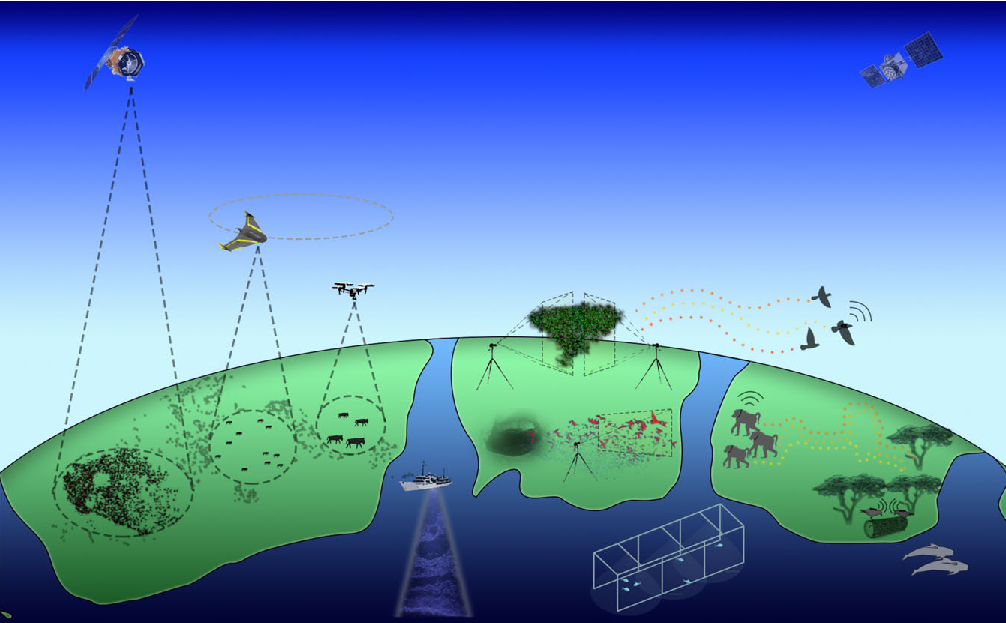
\includegraphics[width=.8\textwidth]{methods_behavioral_studies}}
  \caption{\label{methods_hebavioral_studies} Different methodological approaches emerged from the rapid technological advances of the last decades. Recording devices range from satellites, over unmanned aerial vehicles like drones, to stationary single or synchronized cameras and animal mounted bio-loggers. This huge variety of recording devices enables data acquisition to be adapted to the requirement of a scientific study, i.e. a specific model species, its behavior, the environmental conditions it lives in, and the scientific question that shall be tackled. Taken from \citet{Hughey2018}.}
\end{figure}

However, recent technological advantages in remote recording techniques, tags, and data loggers (\figref{methods_hebavioral_studies}), as well as in associated data processing techniques enable high-throughput studies not only for behavioral sciences but also for ecology and neuroscience \citep{Anderson2014, Dell2014, Hughey2018, Mathis2018}. A benefit of these approaches is that recordings contain rather unspecific data from which all sorts of information can be retrieved after the recordings have been made, including behavioral events or environmental information \citep{Gomez2014}. This allows for post-hoc discoveries of behavioral causalities and the development of associated hypotheses, which has already been demonstrated in research on group coordination in baboons \citep{Strandburg2015} and meerkats \citep{StrandburgPeshkin2019}, as well as reproductive behavior in field crickets \citep{Rodriguez2010}. 

Based on the requirements of a scientific project, i.e. model species, environmental conditions, and scientific question, the most suitable recording technique can be selected from a huge variety of available recording devices \citep{Hughey2018}. Respective methodological approaches can be subdivided into two main categories: Either animals themselves are equipped with bio-loggers or external recording devices are utilized to record their behavior.

\paragraph{Bio-loggers} 

Bio-loggers are small devices that, equipped with a variety of different on-board sensors, get affixed to animals themselves and record different aspects of their behavior or physiological condition \citep{Menzel2005, Baktoft2015, Strandburg2015}. Accordingly, they are most suitable to study highly mobile animals or those who live in remote, hard to access areas. Using this method, many interesting insights into different aspects of natural animal behavior have been gained already, including collective movement \citep{Nagy2010, Strandburg2015}, leadership \citep{Strandburg2018}, or foraging ecology of deep-diving animals (elephant seals: \citealp{Robinson2012}). 

Still, technical limitations of bio-loggers can lead to some issues that can potentially influence scientific validity. Experimenters frequently need to interact with animals (e.g. to mount, recharge, or read-out loggers) and animals are required to carry recording devices. This alone already can result in changes of behaviors, reproduction, or survival, and thus bias observations \citep{Saraux2011}. In order to reduce these biasing factors, different trade-offs regarding sample rate, duty cycling, and battery life are required \citep{Hughey2018}, e.g. the deployment of smaller loggers that have less effects on an animal's natural behavior at the cost of decreased battery capacity or devices recording discontinuously for predetermined time periods in order to reduce energy consumption and therefore the frequency of required interactions with animals (e.g. \citealp{StrandburgPeshkin2017}). Furthermore, not all individuals of a study population can usually be equipped with recording devices (e.g. \citealp{StrandburgPeshkin2019}) and those loggers deployed are limited in their recording range to the direct surrounding of the respective animal. Accordingly, bio-loggers can potentially miss out on recording relevant stimuli that elicit recorded behaviors when (i) stimuli take place off recording cycle or (ii) out of detection range of deployed bio-loggers, with the latter also including (iii) untagged animals. 

These unavoidable trade-offs have the potential to impede the validity of respective studies, which might even remains unnoticed. For example, when conducting behavioral studies in natural populations, possible changes in the composition of the study population have to be regarded, e.g. caused by individuals leaving or joining the group \citep{Janson1985, Engh2002}. Such changes can have tremendous effects on group or individual behaviors \citep{Metcalfe1995, Sapolsky2005}. However, with incompletely tagged groups, the detection of such events can be difficult or impossible and the evaluation of recorded behaviors elicited by such undetected events can lead to the suggestion of false causalities.

\paragraph{Remote-sensing} 
An alternative approach is to refrain from animal mounted bio-loggers and instead detect and track whole populations of animals and their behaviors in external recordings \citep{Hughey2018}. Corresponding devices can be anything capable of recording different aspects of an animal's morphology or behavior, including satellites, unmanned aerial vehicles equipped with on-board sensors (e.g. drones with video cameras), stationary synchronized or single video-cameras, directed microphones, or even arrays of electrodes submerged in the water \citep{Theriault2014, Henninger2018, Hughey2018}. Even though these techniques are sometimes disadvantageous in natural, cluttered environments \citep{Dell2014} the huge versatility of recording devices allows for their utilization in the context of various different studies. Individual flight paths of bats and birds have been reconstructed from video recordings of stationary cameras \citep{Theriault2014}, herds of caribous have been filmed using unmanned aerial vehicles like drones in order to study collective movement and information transfer in groups \citep{Torney2018}, and electric signals of electric fish have been recorded using electrode grids to gain insights into their natural communication and movement behaviors \citep{Henninger2018, Henninger2020}. However, the evaluation of such recordings is way more challenging compared to bio-loggers. Recorded animal signals (e.g. aspects of appearance or emitted signals) need to be detected, classified, and tracked in order to obtain viable behavioral traces. This usually requires custom analysis tools that are adapted to a specific scientific question (e.g. individual or species identification, behavioral classification, etc.).

\paragraph{Laboratory studies} 
Indeed, observations and experiments in an animal's natural environment are indispensable in order to fully understand their behaviors, since only there the entirety of stimuli and circumstances potentially affecting them is available. Nevertheless, laboratory studies are of central interest, too, since they allow for detailed and continuous observations of behaviors in response to well controlled stimuli (e.g. \citealp{Chivers1995, Barber2000, Hupe2008}). Accordingly, causalities between behaviors and different stimuli can easier be identified and described more accurately. However, as mentioned above, behaviors observed in the laboratory often severely deviate from natural behaviors, because of artificial experimental conditions \citep{Henninger2018}. 

Laboratory experiments with long and continuous observation times in semi-naturalistic environments can combine the advantages of well controlled laboratory experiments and field observations. Diverse aspects of an animal's behavior can be observed in depth, while naturalistic environmental conditions ensure behaviors to be much closer to those observed in the wild. Unfortunately, studies of these kind are still rare, though, since handling and analysis of the resulting large and high dimensional data-sets is demanding and challenging \citep{Gomez2014}.

Yet, electric fish are most suitable for such elaborate studies. These fish emit electric signals that can be recorded by means of electrode arrays submerged in the water and used for tracking individual behaviors, including communication \citep{Smith2013} and movement \citep{Madhav2018, Henninger2020}. Since this method is non-invasive, recorded behaviors can be assumed to be most natural, especially when fish are kept under naturalistic conditions. Furthermore, long-term behavioral observations are feasible in these fish since recording duration is only limited by data storage capacities.

\section{Electric fish}

\begin{figure}[h!]
  \centerline{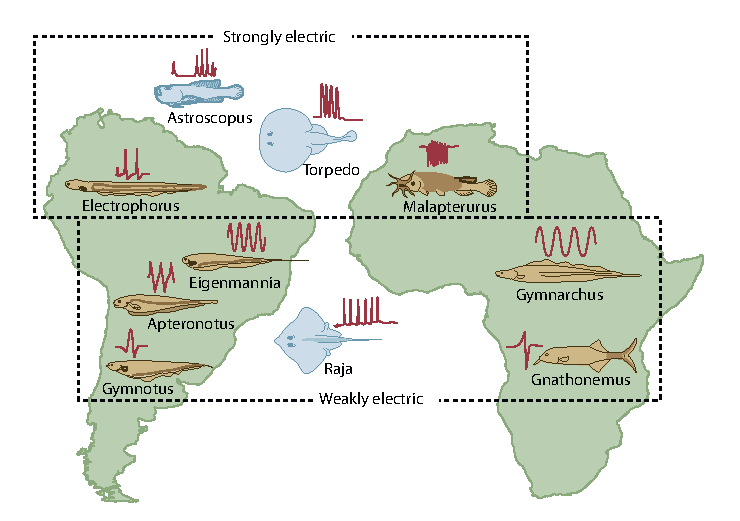
\includegraphics[width=.8\textwidth]{distribution_efish}}
  \caption{\label{efish_dist} Global distribution of electric fish species. Different species can be found in marine (blue) as well as in freshwater (yellow) environments. Species specific EOD wave-forms are above the respective sketches (red). While strongly electric fish are capable to stun their prey, weakly electric fish utilize their electric fields for electrolocation and communication. Taken from \citet{Nelson2011} after \citet{Moller1995}.}
\end{figure}

Two groups of electric fishes (African Mormyriformes and South American Gymnotiformes, \figrefb{efish_dist}) have independently developed electrical organs, producing species specific electric organ discharges (EODs, \citealp{Hopkins1978, Turner2007}), used for electrolocation \citep{Nelson1999, Fotowat2013} and communication \citep{Smith2013}. In particular, Gymnotiform wave-type fish continuously generate EODs with individual-specific frequencies that remain, in constant environments, remarkably stable over many hours and days (\citealp{Bullock1970, Moortgat1998}, \figsrefb{efish_dist}, \subfref{field_simulation}{B}). That is, these fish all “glow” in individual “colors”. By simply recording their electric fields with an array of electrodes submerged in the water -- as has been suggested by \citet{Hagedorn1985} -- these fish can be tracked without the need to tag them or to mount loggers \citep{Jun2013, Matias2015, Madhav2018, Henninger2018, Henninger2020}. Furthermore, electrocommunication signals (see below) are recorded in one and the same channel which is also used for tracking \citep{Henninger2018}. This makes electric fish an advantageous and highly accessible model organism for large-scale and detailed behavioral observations.

Species diverse Gymnotiform fishes (more than 250 species, \citealp{Albert2005, Ferraris2017}) make up to 70\,\% of the biomass of large rivers in South America \citep{Marrero1991, Cox2004, Crampton2011}. However, despite their importance in tropical freshwater ecosystems \citep{Cox2004, Crampton2011} and their extensively studied electrosensory system \citep{Benda2005, Bullock2006, Grewe2017, Sinz2020}, little is known about their ecology, ethology and life history, because field research on these fascinating fishes was, until recently, severely limited by their nocturnal and secretive lifestyles. During the day, electric fish hide at resting sites under submerged logs (Gymnotus, \citealp{Westby1970}), between roots (Eigenmannia, \citealp{Hopkins1974}), within leaf litter (Brachyhypopomus, \citealp{Hagedorn1988}), and even buried in sand (Gymnorhamphichthys, \citealp{Lissmann1965}). During the night, however, these fish become more active: Some species increase their EOD frequency (EODf, \citealp{Lissmann1965, Stoddard2007}), communication signals are produced more frequently \citep{Zupanc2001, Henninger2018}, higher movement activities can be observed \citep{Henninger2020}, and courtship takes place \citep{Hagedorn1985, Henninger2018}. Altogether, a plethora of behaviors and social interactions can be observed in these fascinating animals during the night.

\subsection{\Lepto{} and its social behavior}

\begin{figure}[h!]
	\centerline{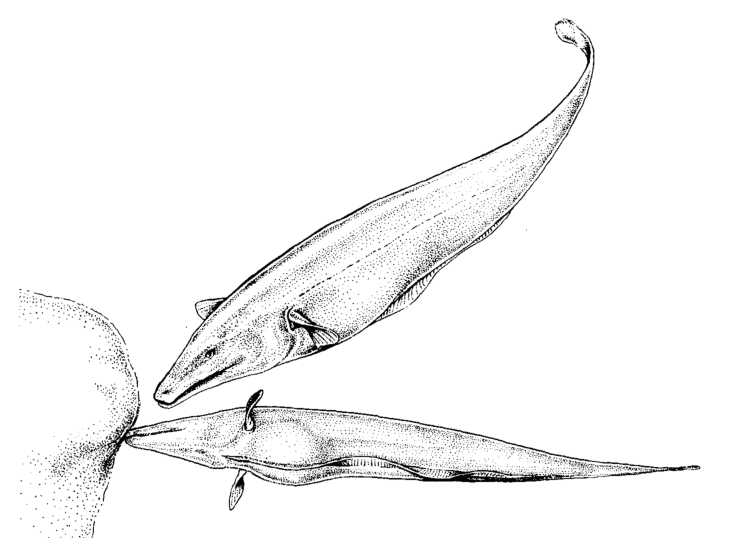
\includegraphics[width=.8\textwidth]{lepto_sketch}}
	\caption{\label{lepto_sketch} Physical appearance and mating behavior of \lepto{}. The characteristic enlarged ribbon fin enables these fish to swim in any direction independent from their orientation and helps them to maneuver in the confined spaces of their preferred natural habitats. Since the corresponding innervating muscles take up most of the caudal part of their  body, the visceral organs, including cloaca and gonads, are concentrated in the rostral body. The displayed behavior corresponds to reproduction. The coordination of females spawning a single egg and males fertilizing it is only one of the many social interactions, where electrocommunication is of central importance. Taken from \citet{Hagedorn1985}.}
\end{figure}

One of these interactions is competition behavior that, in \lepto{}, comprises ritualized fighting accompanied by various electrocommunication signals \citep{Triefenbach2008, Smith2013}. \lepto{} has been shown to mainly rival for optimal shelters whereas during mating season, males additionally compete for females \citep{Hagedorn1985, Dunlap2002, Henninger2018}. In both cases, more dominant individuals seem to have priority access. In staged competitions for single shelters, \citet{Dunlap2002} found more dominant individuals to occupy higher quality shelters, preferably alone, and anecdotal observations in the field and laboratory suggest more dominant males to participate more in reproduction (\citealp{Hagedorn1985, Henninger2018}, \figrefb{lepto_sketch}). 

Many previous studies found evidence for dominance hierarchies across populations of various electric fish species \citep{Dunlap2002, Stamper2010, Fugere2011, Silva2012}. Even though body size has been shown to be the main determinant for dominance and the outcome of associated competitions \citep{Dunlap2002, Triefenbach2008, Silva2012}, the influence of other factors including sex and the emission of various signals still remains unclear. Especially the role of an individual's EODf as indicator for dominance is discussed controversially. For \lepto{}, some studies found dominance to correlate with EODf in males, but not in females \citep{Hagedorn1985, Dunlap2002}; a finding that has been reproduced in a wild population of Sternarchorhynchus \citep{Fugere2011}. However, in males EODf also correlates with body size, and could therefore be a secondary characteristic of dominance \citep{Dunlap2002, Triefenbach2008, Fugere2011}. Furthermore, some studies suggest female electric fish to either form no dominance hierarchy at all \citep{Hagedorn1985} or only a very distinct one, whereby females with lower EODf are more likely to be found outside of shelter tubes \citep{Dunlap2002}. Other studies suggest dominance to be independent of sex \citep{Silva2012, Zubizarreta2020}. 

\subsection{Electrocommunication}

\begin{figure}[h!]
	\centerline{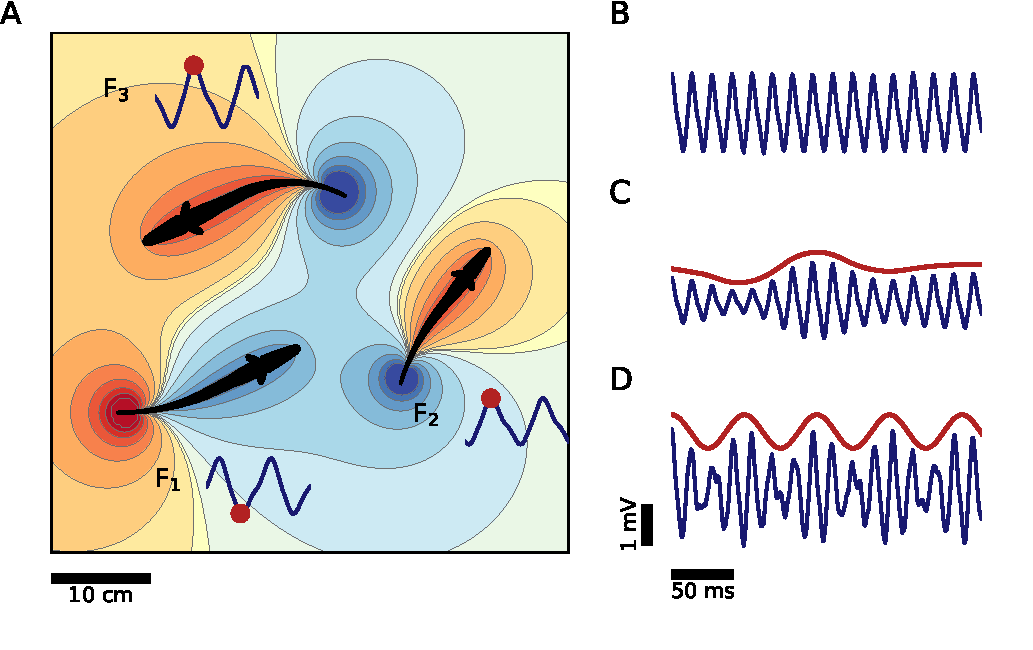
\includegraphics[width=.9\textwidth]{field_simulation}}
	\caption{\label{field_simulation} Electric field characteristics and interactions in electric fish \figitem{A} Electric fields of different fish superimpose and influence each others spatial properties. For each fish the current extend and direction of its electric field is dependent on the phase of its EODs (red marker in black EOD waveform). In the displayed state, the electric field of fish F$_1$ is anti-phasic to those of fish F$_2$ and F$_3$. However, this is only a short lasting state since each fish emits its EODs at an individual specific frequency (EODf). \figitem{B} EODfs of single individuals remain remarkably stable over minutes, hours, and days. \figitem{C} Amplitude modulations (AM) of a single electric field recorded via external recording electrodes or perceived by other electric fish resemble the movements of the respective fish. The amplitude of an electric field decays exponentially with distance to the receiver \citep{Benda2020}. \figitem{D} When two (in the purpose of simplification) stationary electric fields superimpose, the frequency of the resulting amplitude modulation, also called beat, corresponds to the difference frequency between the two original signals. Characteristics of the beat, i.e. its frequency and amplitude, are an important source of social information for electric fish since it resembles a conspecific's identity (individual specific EODf), its movement behavior (AM), and even its communication behavior (EODf changes).}
\end{figure}

Electrocommunication is used in various social contexts across electric fish species \citep{Westby1970, Hupe2008, Silva2012, Smith2013}. Especially \lepto{} is known for its rich repertoire of various electrocommunication signals \citep{Smith2013}, e.g. employed in courtship \citep{Hagedorn1985, Henninger2018} and agonistic contexts \citep{Hupe2008, Triefenbach2008}. Wave-type electric fish already gather relevant information about each other by means of perceived structural changes of their own electric field resulting from the interactions with electric fields of other fish (\subfigref{field_simulation}{A}). The electric fields of two wave-type fish superimpose and result in a beat, i.e. a periodic amplitude modulation of the receiver's electric field. 

The amplitude of the beat indicates the distance between fish, whereas the frequency of the beat equals the difference between the two EODfs (\citealp{Henninger2020}, \subfigrefb{field_simulation}{C, D}). Both amplitude and frequency of amplitude modulations are encoded by electroreceptor afferents of the active electrosensory system \citep{Benda2006, Hupe2008b, Walz2014}. In the \lepto{} species group \citep{DeSantana2013}, EODf is sexually dimorphic with females having lower frequencies (600--750 Hz) than males (750--1000 Hz, \citealp{Meyer1987}). Thus, beat frequencies convey information about species affiliation and sex of another fish, e.g. if it is a competitor for limited resources or a potential mating partner, but this information is ambiguous \citep{Henninger2018, Henninger2020}. Because of the beat, conspecifics can detect each other over a distance of up to two meters \citep{Knudsen1975, Henninger2018, Henninger2020} and potentially assess each other's sex and dominance, as well as monitor each other's movement behaviors \citep{Davies1978, Fernald2014}. At the same time, low-frequency beats have been suggested to jam electrolocation signals \citep{Bastian1987}, posing a potential limiting factor to group density.

\begin{figure}[tp]
  \begin{minipage}[t]{0.45\textwidth}\mbox{}\\[-2ex]
    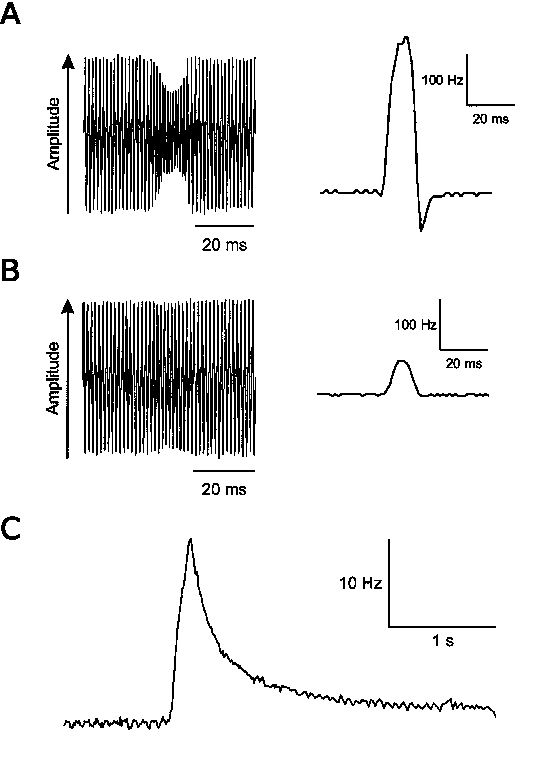
\includegraphics{e_communication}
  \end{minipage}
  \hfill
  \begin{minipage}[t]{0.35\textwidth}
  \caption{\label{e_com_sigs} Electrocommunication signals commonly emitted by \lepto{}. \figitem{A} Type-1 chirps are characterized by an EODf increase of up to 200\,Hz and a frequency undershot before returning to baseline EODf. While the chirp is emitted, the EOD amplitude is temporarily decreased. Type-2 chirps can best be elicited with EODs with large EODf difference, hinting towards their importance in inter-sex interactions. \figitem{B} Type-2 chirps are smaller in their frequency excursion and do not come with a decreased EOD amplitude. These chirps are emitted during agonistic interactions, but also during courtship. \figitem{C} Rises are characterized by rapid increases in EODf by a few tens of Hertz followed by an exponential decay back to baseline EODf. The significance of these signals is discussed controversially throughout the literature. Taken from \citet{Zupanc2002}.}
  \end{minipage}
\end{figure}

Wave-type Gymnotiform fish generate three distinct types of communication signals by actively modulating their EODf: Chirps, rises, and jamming avoidance responses \citep{Engler2000, Zakon2002}. Chirps are brief temporal frequency excursions ranging from 70\,Hz up to more than 400\,Hz with a duration of approximately 30\,ms to 500\,ms \citep{Engler2000} that transiently advance the phase of the ongoing beat \citep{Benda2005}. For \aptero{}, at least two types of chirps are known \citep{Hagedorn1985, Dunlap2003b, Henninger2018}. A small chirp (50--150\,Hz, \subfigrefb{e_com_sigs}{B}) is associated with agonistic, same sex interactions \citep{Smith2013}, but is also used during courtship to synchronize spawning \citep{Henninger2018}. A large chirp (200--400\,Hz, \subfigrefb{e_com_sigs}{A}) is predominantly produced by males in response to electric fields belonging to potential mating partners \citep{Triefenbach2003}. In \rostratus{} and \lepto{}, females exclusively produce a special long chirp when ejecting a single egg \citep{Hagedorn1985, Henninger2018}. However, it is important to note that most of the knowledge on chirps is based on laboratory experiments in more or less artificial and restricted settings (e.g. \citealp{Engler2001, Dunlap2003b, Zupanc2006, Hupe2008}). Those settings turned out to evoke chirping behaviors quite distinct from field observations or long term laboratory breeding experiments \citep{Henninger2018}. 

Another category of electrocommunication signals, EODf rises, are characterized by a rapid but moderate increase in EODf by no more than a few tens of Hertz followed by an exponential decay back to baseline EODf within a few seconds (\citealp{Hagedorn1985, Engler2000, Zakon2002}, \subfigrefb{e_com_sigs}{C}). The frequency increase and duration of rises are highly variable within species, but seem to be conserved across species and sexes \citep{Turner2007}. The function of EODf rises is discussed controversially \citep{Smith2013}. Rises have been suggested to be signals of dominance \citep{Tallarovic2005}, appeasement signals produced by subordinate fish \citep{Serrano2003}, context specific signals produced by subordinates and dominants \citep{Hopkins1974}, or just a general expression of stress \citep{Smith2013}.

Finally, in \Eigenmannia{}, electrolocation performance is impaired by the presence of a conspecific with a similar EODf \citep{Heiligenberg1973} because the resulting low-frequency beat shadows signals evoked by objects \citep{Behrend1977}. By means of the jamming avoidance response, \Eigenmannia{} changes its EODf in a way that the beat frequency is increased \citep{Watanabe1963, Bullock1969} and, thus, a jamming signal is moved outside the frequency band relevant for electrolocation \citep{Nelson1999, Fotowat2013}. In contrast, \aptero{} only increases EODf when jammed \citep{Heiligenberg1996}, which does not necessarily result in an increase of beat frequency, but instead sometimes actively jams a conspecific \citep{Tallarovic2005, Triefenbach2008}. The latter behavior might be considered a communication signal. However, its importance still remains to be determined.

\section{Aim of the study}

\lepto{} has been a successfully established model species in neuroscience for several decades. Even though their electro-sensory system is among the best described neuronal pathways (e.g \citealp{Benda2005, Bullock2006, Sinz2020}), little is known about their natural behaviors, including their social organization. Only few previous studies investigated behavioral topics like shelter occupation \citep{Dunlap2002, Stamper2010}, short competitions \citep{Hupe2008, Triefenbach2008}, dominance \citep{Dunlap2002}, and electrocommunication \citep{Smith2013, Henninger2018}, especially with chirps \citep{Engler2000}. Furthermore, most of these studies have been conducted in confined laboratory settings with reduced, artificial environments and short observation times. Accordingly, the interpretations of observed behaviors and suggested causalities are often conflicting between studies, but nevertheless provide a strong basis. Indeed, some studies started to evaluate behaviors of \lepto{} in the wild, focusing especially on movement patterns and intra-specific communication with chirps in the context of reproduction and aggression \citep{Henninger2018, Henninger2020}. However, in these studies the dimensionality of firm conclusions about the social organization in \lepto{} is limited since they lack information about the observed animal's physical conditions, life history, and long term behavioral traits (fish frequently leave observation areas and are impossible to reidentify). Many mysteries about their secretive life still remain unresolved: What form of social organization prevails in populations of \lepto{}? What external and internal motivators drive decision making during competitions for resources and dominance? What are behavioral manifestations of dominance? What is the meaning of the various electrocommunication signals involved in all kinds of social interactions?    

To explore these questions my thesis pursued two main objectives. First, I developed the methods and algorithms required for tracking EODs of individual wave-type electric fish recorded with electrode arrays in different laboratory and natural settings (\chapref{Methods}). I combined and refined previous approaches \citep{Madhav2018, Henninger2020} and thereby developed a semi-automatic system capable of tracking electric fish with unprecedented accuracy. This advanced tracking approach, accordingly, also reduces the expense of required post-processing and therefore facilitates long-term observation studies on electric fish in more naturalistic settings, i.e. when many with potentially similar EODfs are recorded simultaneously.

Subsequently, I applied the developed methods to observe and evaluate behaviors of freely moving and interacting \lepto{} in different settings. In order to gain a comprehensive understanding about the meaning and causalities of the various social behaviors of \lepto{}, I combined behavioral observations in naturalistic settings with controlled laboratory experiments. In a large laboratory aquarium containing several naturalistic habitats and shelters, I evaluated individual spatio-temporal behaviors in a population of 14 \lepto{} in order to tackle questions regarding habitat preference and group dispersion, as well as how a fish's spatio-temporal behavior is affected by its social status (\chapref{Habitats}, \citealp{Raab2019}). In a subsequent experiment, I analyzed behaviors and interactions of unfamiliar pairs of \lepto{} during staged competitions, e.g. when fish first try to establish dominance (\chapref{Competitions}, \citealp{Raab2021}). In this experiment, my main objective was to identify which individual characteristics or physical attributes of fish are decisive for the outcome of competitions, how fish assess opponents, and how this assessment manifests behaviorally. Another aim of this study was to identify the meaning of electrocommunication with rises during social encounters, especially in the context of agonistic interactions. 


%\bibliographystyle{jneurosci}
%\bibliography{../journalsabbrv,../references}

\cleardoublepage
\graphicspath{{chapter_2_methods/figures/}}
\chapter{Semi-automatic tracking of wave-type EODs}
\label{Methods}

\section{Introduction}

Clearly determining the causalities of animal behaviors in experimental or observational studies is often challenging, since animals are sensitive to a broad range of stimuli. Certain behaviors can, for example, be elicited by different social and environmental stimuli or be influenced by an animal's current internal state \citep{Chapman1995, Sapolsky2005, Boon2007, Markham2015}. Regarding all these influencing factors in a single scientific project is certainly difficult, if not impossible. Laboratory studies usually tackle this issue by reducing experimental environments and thereby the scope of factors potentially influencing behaviors (e.g. mice startle response, \citealp{Pantoni2020}; evoked communication in electric fish, \citealp{Bastianetal2001}). Such studies are, accordingly, most suitable to describe and evaluate causalities between specific behaviors and well defined stimuli in detail. On the other hand, their potential to discover unexpected behavioral traits and causalities is limited by their reduced experimental framework. Furthermore, since behaviors observed in the laboratory often deviate from those observed in the wild \citep{Cheney1995, Rendall1999, Henninger2018}, field studies or laboratory experiments with complex, more naturalistic designs are essential to gain a comprehensive understanding of an animal's natural behavior. Only in such settings the whole range of an animal's behavior can be observed and the validity of laboratory observations can be certified. 

The greatest challenge of such elaborate studies is the collection of comprehensive and viable data, including detailed observations of animals and their behaviors but also information about their surrounding environment. However, recent technological advances in remote recording techniques, tags, and data loggers allow for elaborate studies with freely moving and interacting animals in naturalistic settings \citep{Hughey2018, Mathis2018}. Recording devices got cheaper, smaller, and more energy efficient \citep{Hughey2018, Jolles2021} and our capabilities to analyze corresponding recordings greatly expanded and improved \citep{Dell2014}. A benefit of these approaches is that recordings contain rather unspecific data from which all sorts of information can be retrieved after the recordings have been made, including behavioral events or environmental information \citep{Gomez2014}. 

% Bio-loggers
Based on the requirements of a scientific project, i.e. model species, environmental conditions, and the scientific question, the most suitable recording technique can be selected from a huge variety of available devices \citep{Hughey2018}. For example, in studies on highly mobile animals or those who live in remote, hard to access areas, bio-loggers are most suitable to collect viable behavioral data \citep{Nagy2010, StrandburgPeshkin2017}. Bio-loggers are small recording devices that get affixed to animals themselves and can be equipped with a variety of different on-board sensors, like GPS, magnetometers, pressure sensors, microphones or even video cameras \citep{Hughey2018}. With the help of bio-loggers, many interesting insights into different aspects of natural animal behavior have already been gained, including collective movement \citep{Nagy2010, Strandburg2015}, leadership \citep{Strandburg2018}, or foraging ecology of deep-diving animals (elephant seals, \citealp{Robinson2012}).

Nevertheless, in studies utilizing bio-loggers, experimenters frequently need to interact with animals (e.g. to mount, recharge, or read-out loggers) and animals are required to carry recording devices. This alone already can result in changes of behaviors, reproduction, or survival, and thus bias observations \citep{Saraux2011}. In order to reduce these biasing factors, different trade-offs regarding sample rate, duty cycling, and battery life are required \citep{StrandburgPeshkin2017, Hughey2018}. Furthermore, not all individuals of a study population can usually be equipped with recording devices (e.g. \citealp{StrandburgPeshkin2019}) and those loggers deployed are limited in their recording range to the direct surrounding of the respective animal. Accordingly, bio-loggers can potentially miss out on recording relevant stimuli that elicit recorded behaviors when  (i) stimuli take place off recording cycle or (ii) out of detection range of deployed devices, with the latter also including (iii) untagged animals. 

% Remote sensing
An alternative approach for behavioral studies in naturalistic, open space environments is to detect and track animals and their behaviors in external recordings \citep{Kuhl2013, Hughey2018}. Since interactions with animals are not required for this approach, external influences on their behaviors are minimized \citep{Saraux2011}. Furthermore, the range of feasible behavioral studies is extended to also include animal species that are hard or impossible to access. For example, herds of caribous have remotely been filmed using unmanned aerial vehicles like drones and analyzed in the context of collective movement and information transfer in groups \citep{Torney2018}, individual flight paths of bats and birds have been reconstructed from video recordings of stationary cameras \citep{Theriault2014}, and electric signals of electric fish have been recorded using electrode arrays submerged in the water and analyzed to gain insights into their natural communication and movement behaviors \citep{Henninger2018, Henninger2020}. 

% animal biometrics
However, the analysis of such recordings is way more challenging compared to bio-logger approaches. The methods comprised in a ``biometric system'' usually include algorithms to detect certain animal biometrics, i.e. manifestations of an animal's appearance and/or behavior in such recordings, and compare them to predefined biometric profiles corresponding to the typical manifestation of these biometrics in, for example, a certain species, individual, or behavior \citep{Gaston2004, Sherley2010, Kuhl2013}. In order to enable reliable classification, utilized biometrics need to be universally displayed, while showing sufficient variation between biometric profiles. For example, coat patterns of zebras \citep{Lahiri2011} or the configuration of dark spots on penguin bellies \citep{Sherley2010} are suitable biometrics to reliably identify individuals (biometric profiles). Yet already the reliable detection of selected animal biometrics can be challenging, since individuals can temporarily leave observation areas or the detection of biometrics may fail because of low signal-to-noise-ratios. Further algorithmic challenges can arise from ambiguous biometric profiles. The selection of animal biometrics that can be extracted from recordings is usually limited, which potentially reduces the specificity of biometric profiles. Because of these limitations, biometric profiles are often time-variant and/or overlap in their characteristics, e.g. when using an animal's spatial position for individual identification and tracking (e.g. \citealp{Madhav2018}).

% Electric fish
Based on the general idea of a biometric system, we developed methods and algorithms capable of tracking individual behaviors in freely moving groups of the electric fish \Lepto{}. These fish produce a semi-sinusoidal electric field through continuous discharges of an electric organ (EOD, \citealp{Turner2007}) used for electrolocation \citep{Fotowat2013} and communication \citep{Albert2005, Smith2013}. In order to track electric signals of individual fish, we take advantage of the different characteristics of their EODs that can be extracted from recordings of electrode arrays submerged in the water \citep{Jun2013, Madhav2018, Henninger2018, Raab2019}. 

Previous approaches already tracked electric signals of individual fish by means of their individual specific EOD frequency (EODf, \citealp{Henninger2020}) or spatial electric field properties that can be reconstructed from signal powers across recording electrodes \citep{Madhav2018}. However, the latter depends on the fish's spatial position and orientation and even though individual specific EODfs are remarkably stable over minute to hours \citep{Moortgat1998}, they are sensitive to temperature changes and can be altered actively in the context of communication \citep{Dunlap2000, Smith2013}. Accordingly, these signal features can temporarily overlap between individuals, which complicates reliable tracking, especially for recordings of electric fish in high densities.

In the following sections, we describe and evaluate a new approach for analyzing the electric signals of whole populations of wave-type electric fish recorded with electrode arrays in different configurations. By combining, refining, and extending previous approaches, our algorithm is capable of tracking EODs of individual fish with unprecedented accuracy. Since various different behavioral traits of these fish, including communication \citep{Smith2013} and movement behaviors \citep{Madhav2018}, can be evaluated base on their EODs, our algorithms are a fundamental advancement for various different behavioral studies on freely moving and interacting electric fish \citep{Raab2019, Raab2021}.

\section{Data acquisition}

We developed an easy to modify recording setup that can be adapted, scaled, and adjusted according to the conditions of different experimental settings, e.g. varying environments or observation areas. All recording setups described below are powered by car batteries (12\,V, 80\,Ah) which reduces the influence of electric noise of line current and enables recordings even in hard to access areas, e.g. remote rivers in South America. The core element of the setup is its array of monopolar electrodes at low-noise buffer headstages (1$\times$gain, 10$\times$5$\times$5\,mm$^3$, \subfigrefb{setup_n_trace}{B}) arranged in grid-like structures (\subfigref{setup_n_trace}{C, D}). Electric signals are amplified (100$\times$gain, 100\,Hz high-pass filter, 10\,kHz low-pass), digitized at 20\,kHz with 16 bit resolution, and stored on external data storage devices for later offline analysis. Various electrode grid configurations have already been successfully applied to record populations of electric fish in the wild (\citealp{Henninger2018, Henninger2020}, unpublished field-trips: Colombia 2016, 2019, \subfigrefb{setup_n_trace}{C, E}), as well as in the laboratory (\citealp{Raab2019, Raab2021}, \subfigrefb{setup_n_trace}{D, F}). While the core element of the recording setup with its multiple electrodes and the configuration of amplifiers have remained unaltered during about a decade of electrode-grid based electric fish research, the hardware used for data handling and storage has been revised and improved along the way. The initial computer-amplifier system has been replaced with a more convenient and easy to operate system based on a Raspberry Pi (npi-electronics GmbH, Tamm, Germany, \subfigrefb{setup_n_trace}{A}). The recording software has also remained similar over the years except for being ported from C++ (\url{https://github.com/bendalab/fishgrid}) to Python 3.8 (\url{https://whale.am28.uni-tuebingen.de/git/raab/Rasp_grid.git}) and being more intuitive to handle, e.g. recording configurations can be set using a GUI.

\begin{figure}[h!]
  \centerline{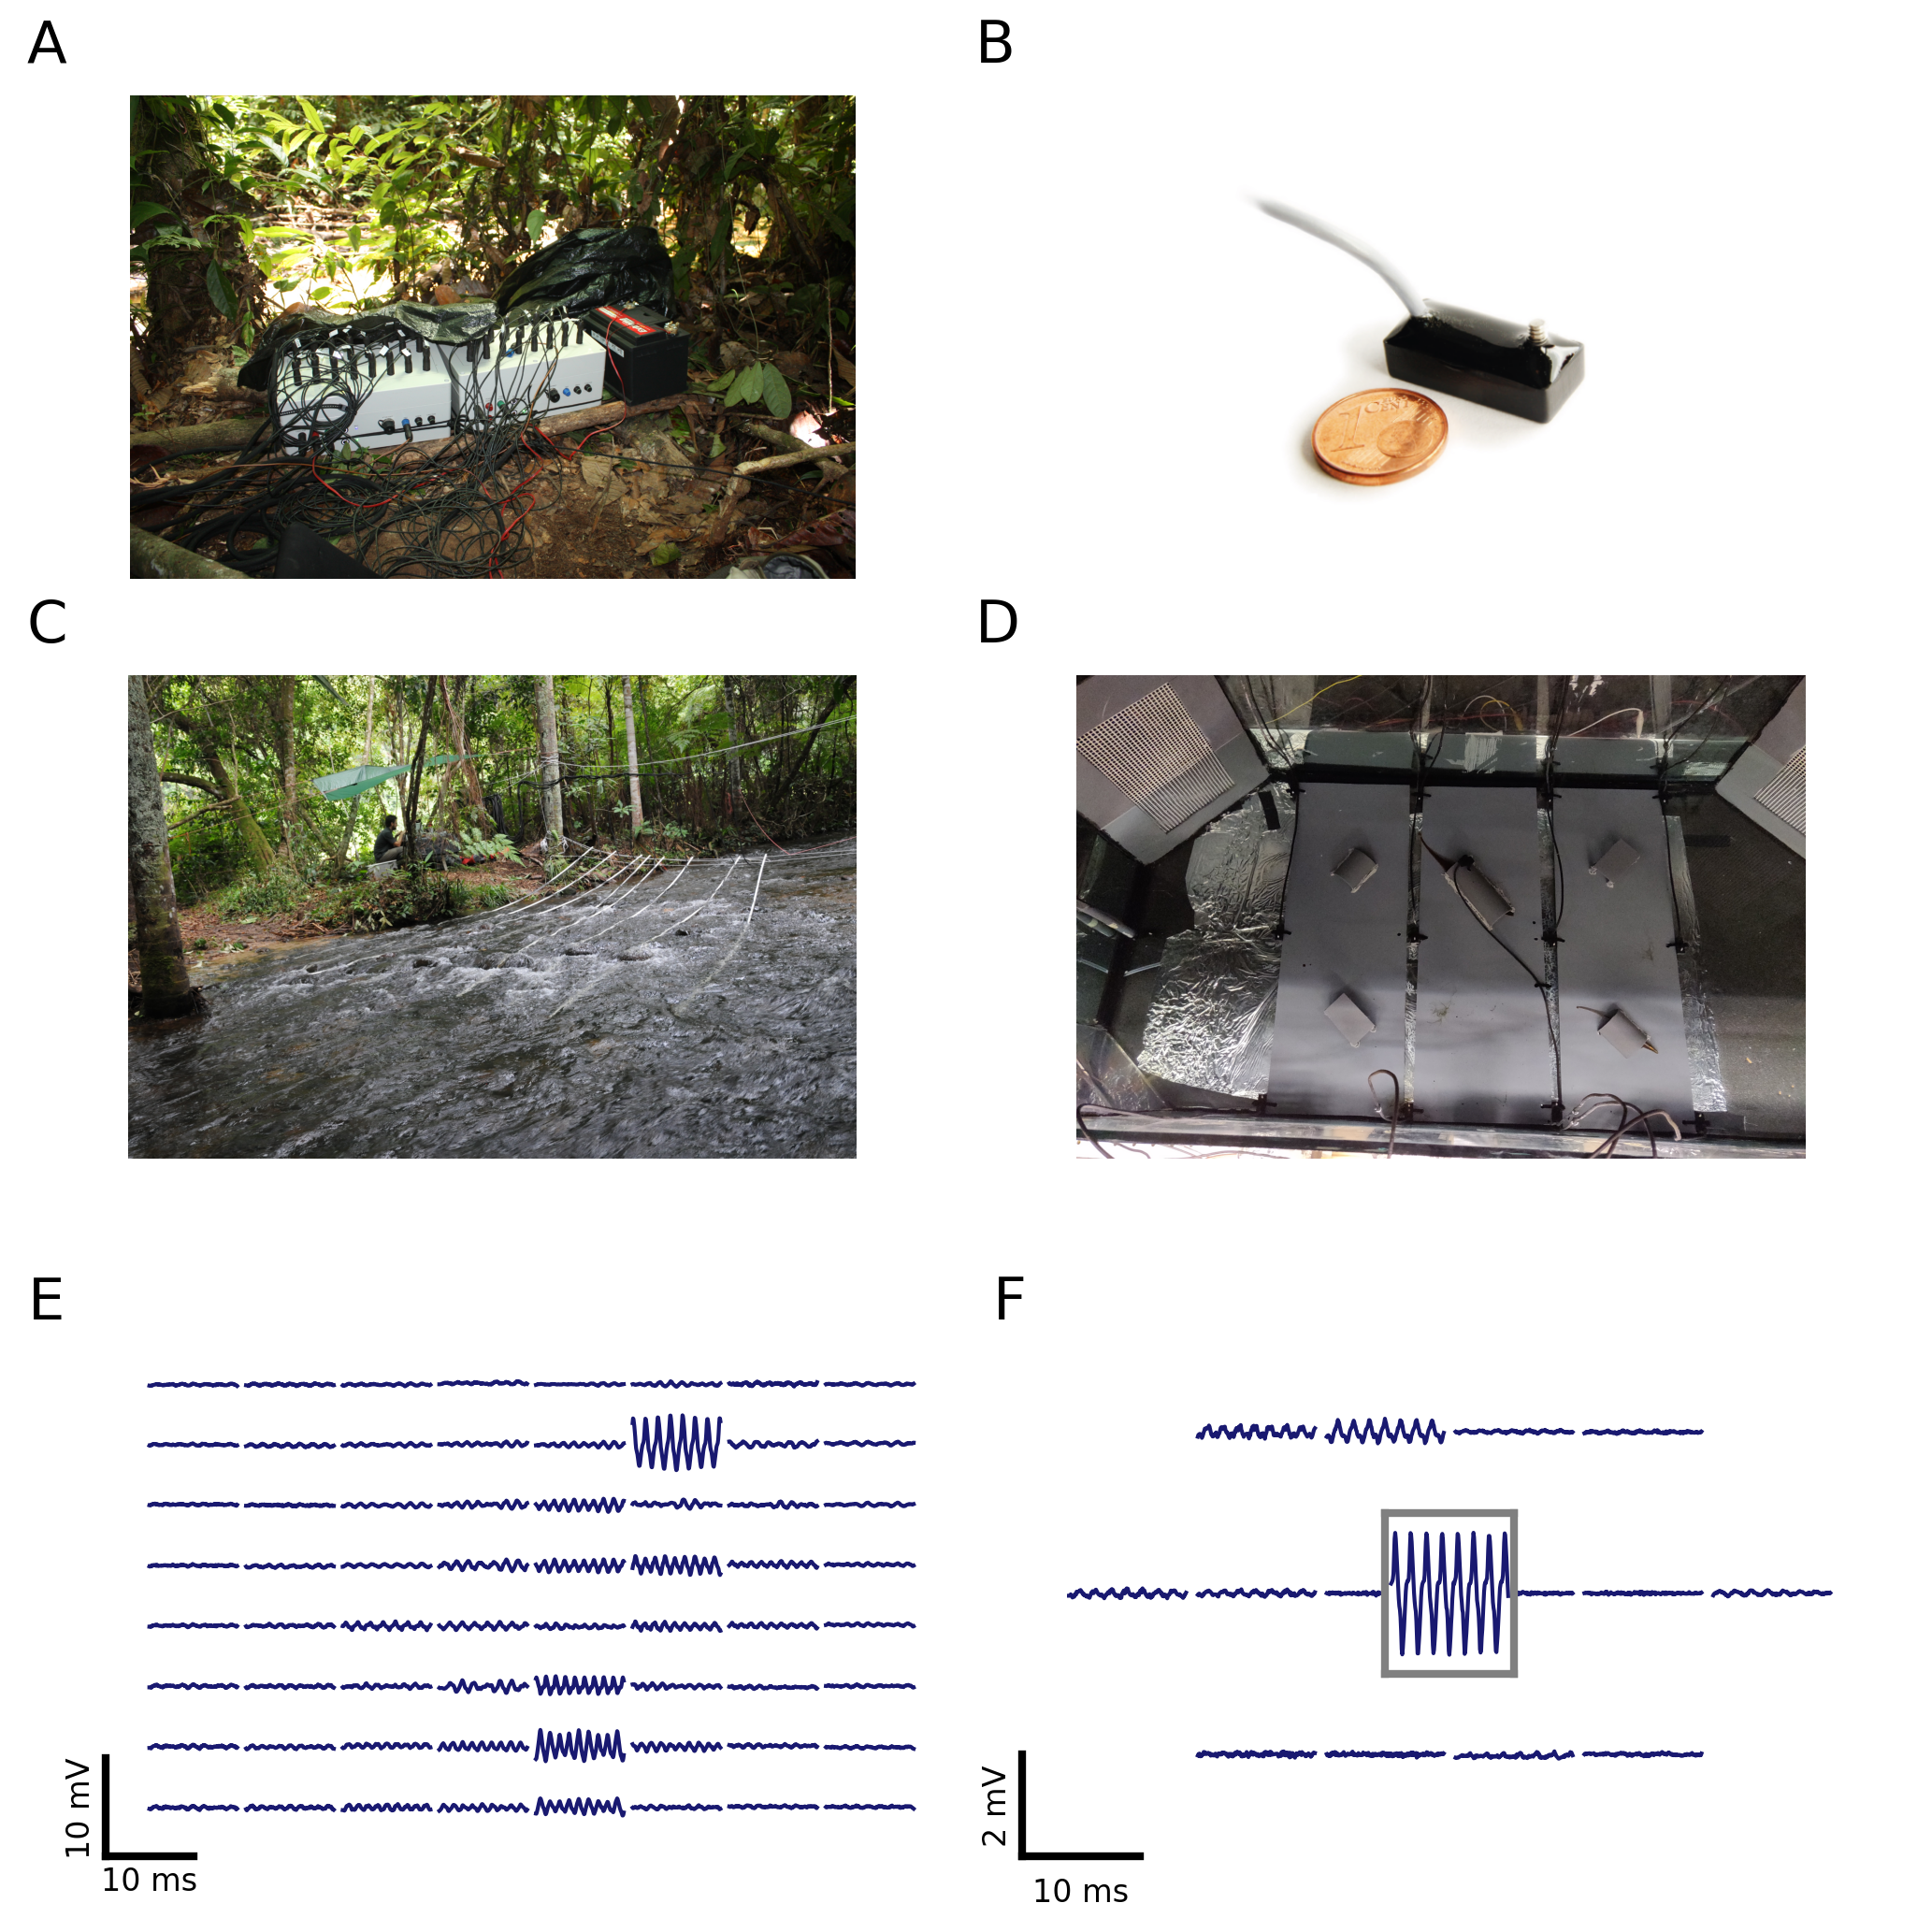
\includegraphics[width=.8\linewidth]{setups_and_raw_traces_new}}
%  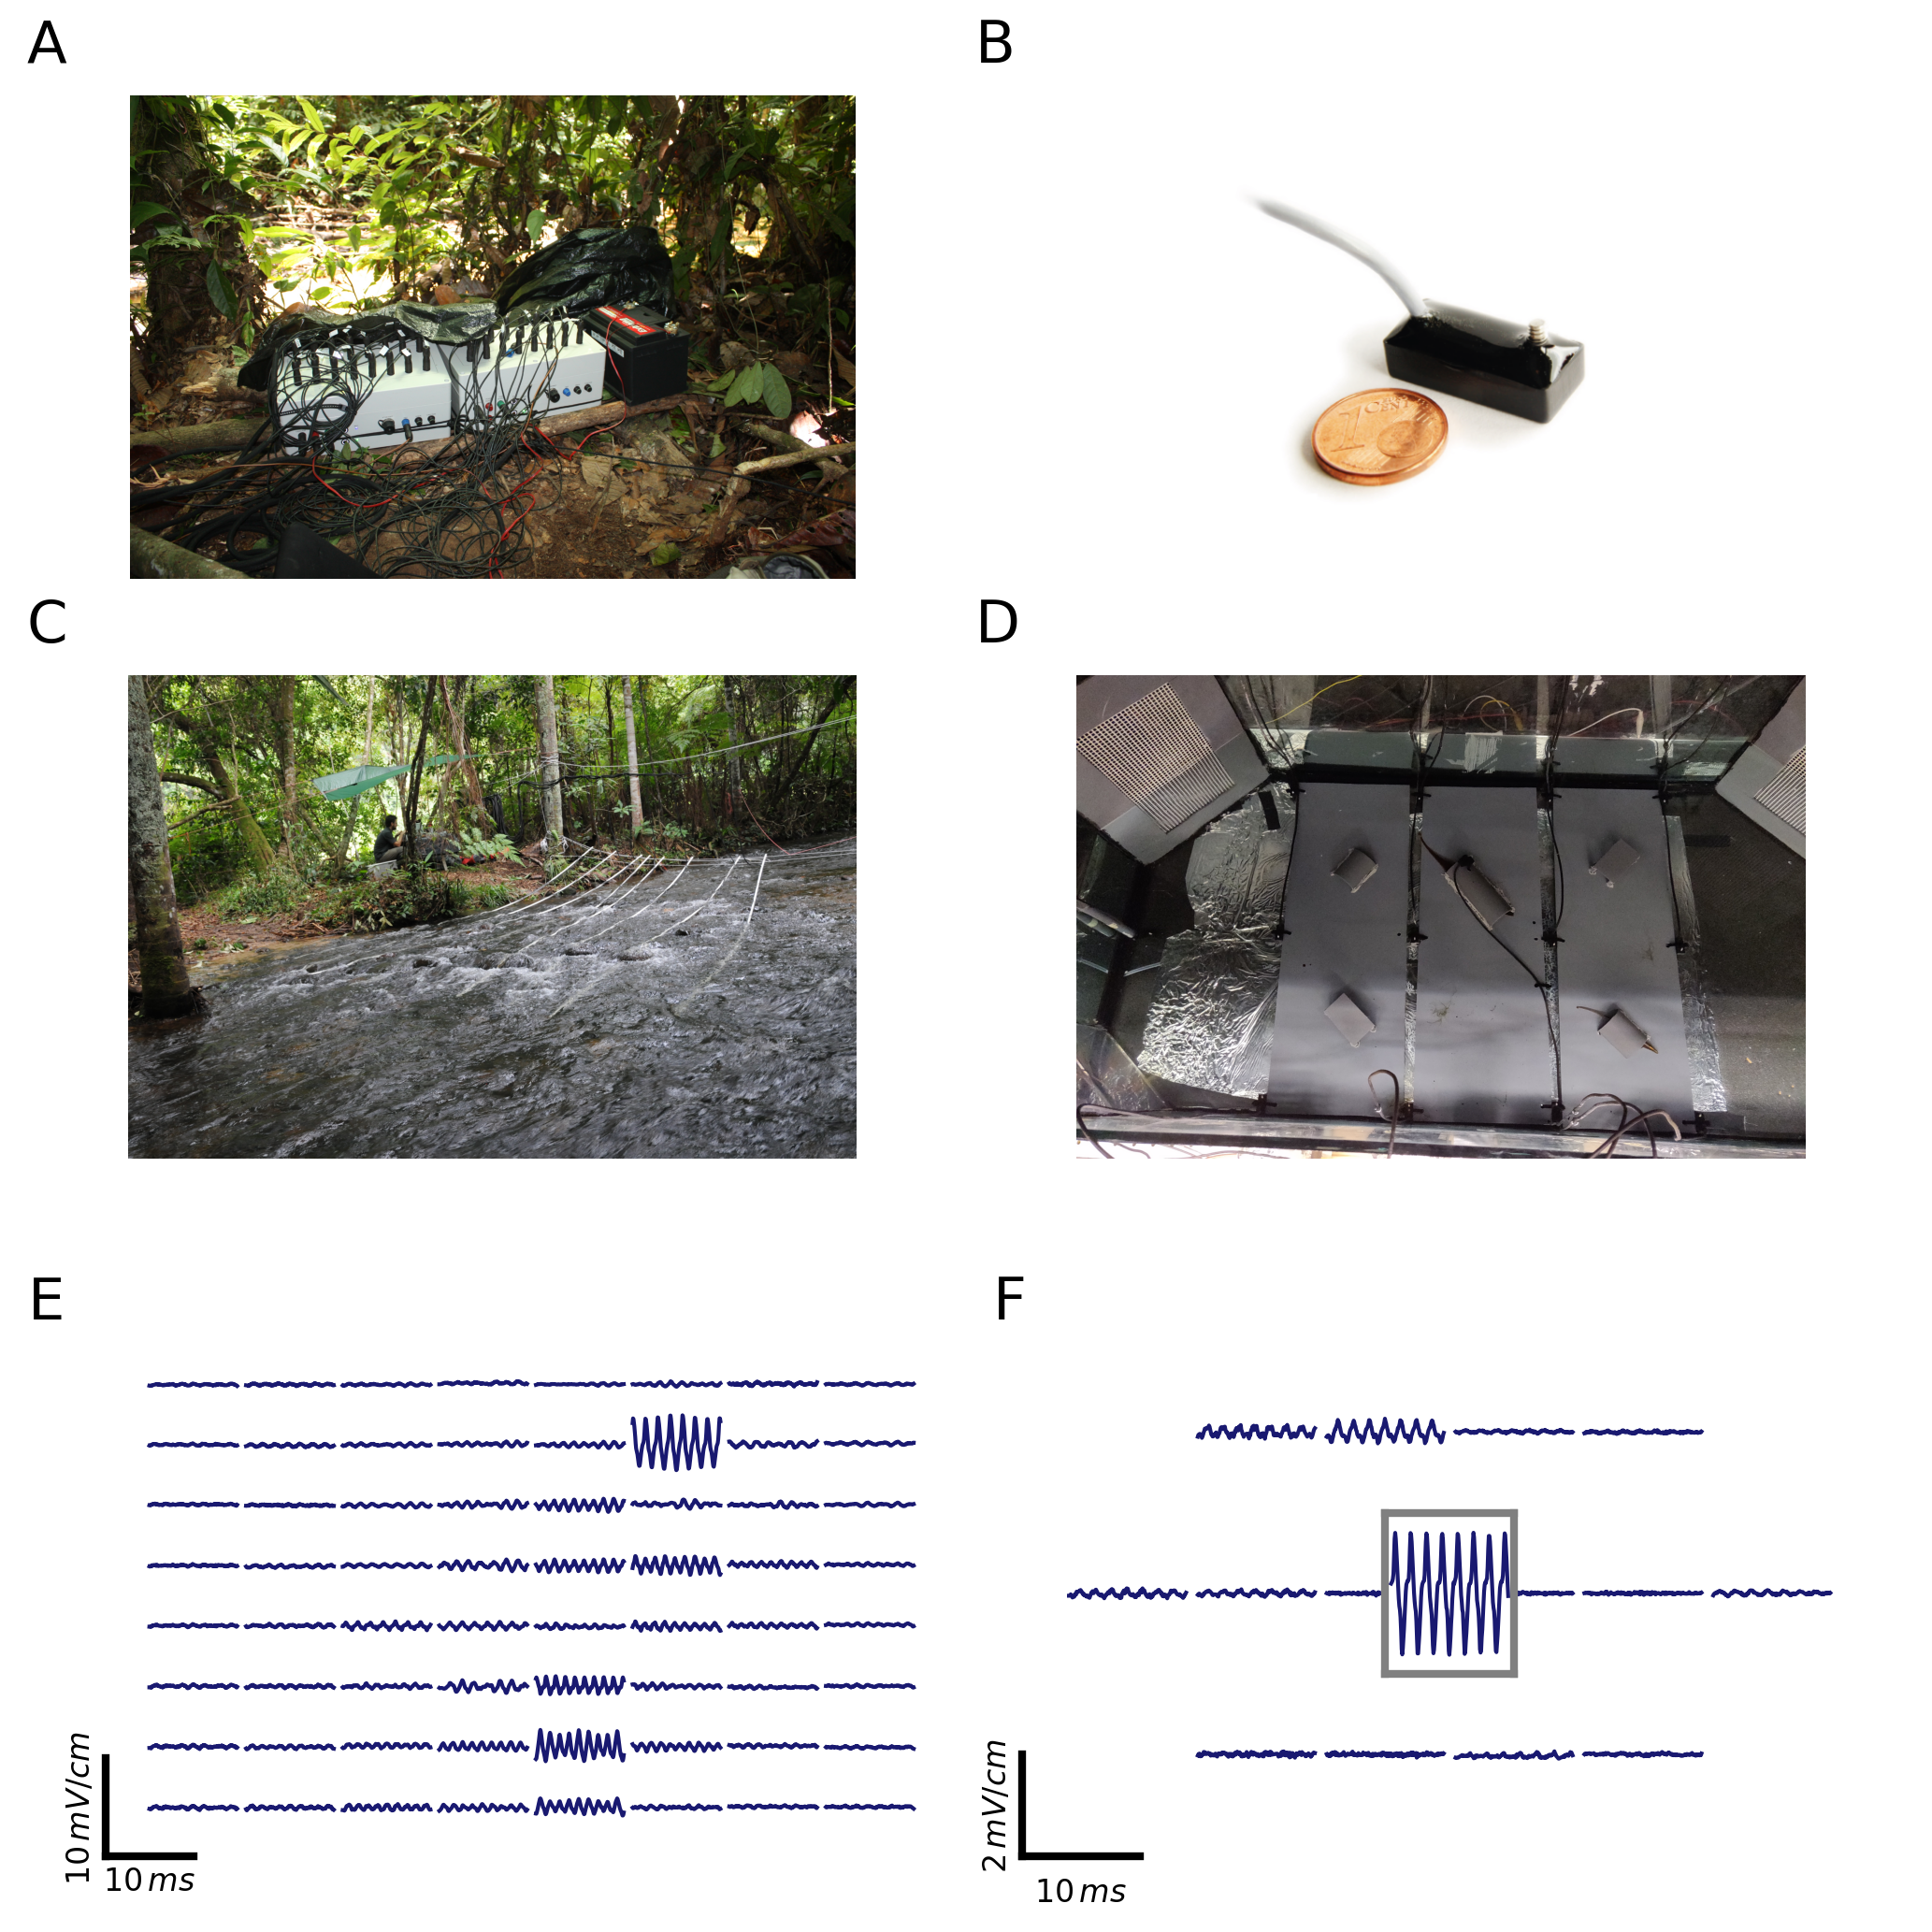
\includegraphics[scale=0.75]{setups_and_raw_traces}
  \caption{\label{setup_n_trace} Recording systems, electrode arrangements, and corresponding signals of recorded electric fish. \figitem{A} The latest version of the recording system enabling simultaneous recording with 16 electrodes. \figitem{B} Monopolar recording electrodes used for recordings in the field and laboratory experiments (after \citealp{Henninger2015}). \figitem{C} Recording setup used to record a population of \lepto{} in the Rio Rubiano, Colombia, in 2016. 64 electrodes were mounted on PVC-tubes and arranged in a 8$\times$8 grid covering an area of 3.5$\times$3.5\,m$^2$. \figitem{D} Recording setup used to record electric signals of pairs of \lepto{} during competitions in a laboratory experiment. 15 electrodes were equally distributed throughout the aquarium to ensure continuous detection of both individual's electric fields. \figitem{E} Snapshot of the electric signals recorded in Rio Rubiano, Colombia, in 2016 with the setup shown in panel~\panel{C}. \figitem{F} Snapshot of electric signals emitted during dyad interactions of \lepto{} in the competition experiment shown in panel~\panel{D}. The signal framed in grey corresponds to the signal recorded by the central electrode located in the long tube in the center of the aquarium (panel~\panel{D}). The EOD of the corresponding \lepto{} shows the characteristic shoulder in each EOD period.}
\end{figure}

%\section{Signal extraction and tracking}
%
%\subsection{Signal extraction}

\section{Detection of individual electric signals (EODs)}

EODs of individual fish are identified and extracted from the electric recordings based on their EODf and respective harmonic structure (\subfigref{signal_extraction}{C}). For each electrode, we compute power spectral densities (PSDs) of overlapping data snippets shifted by $\Delta t$\,$\approx$\, 300\,ms (\subfigref{signal_extraction}{A}). The size of fast Fourier transform windows (nfft) and their overlap represent the trade-off between frequency and temporal resolution. In our analysis, we set both parameters to obtain a temporal resolution of $\Delta t$\,$\approx$\, 300\,ms according to the formula
\begin{equation}
\Delta t = \frac{\text{nfft}}{f_s} \cdot (1-\theta) 
\end{equation}
with nfft being the size of the fft-windows, $f_s$ the sampling-rate of the recording electrodes, and $\theta$ the overlap fraction of fft-windows. 

When we aim for reliable and continuous EODf detection in recordings featuring fish in high density, large fft-windows with more overlap (nfft$=2^{16} \approx$  3.28\,s; $\theta$ = 0.9) are required to resolve EODf differences occasionally dropping below 1\,Hz (e.g. \citealp{Raab2019}). In contrast, smaller fft-windows with less overlap are more suitable when the temporal resolution of electrocommunication signals is prioritized, e.g. in recordings of dyad interactions during competitions (nfft$=2^{15} \approx  1.64$\,s; $\theta$ = 0.8, \citealp{Raab2021}). 

In order to detect the individual specific EODfs of all recorded fish simultaneously, we sum up PSDs referring to the same time point (t$_i$) across electrodes (\subfigref{signal_extraction}{B}). Peak frequencies are detected in the summed up PSDs after logarithmic transformation \citep{Todd1999, Henninger2020} using the formula
\begin{equation}
L = 10 \cdot log(P/p_0)
\end{equation}
with $P/p_0$ being the powers of frequency ($P$) in the Fourier transformed data relative to a reference power of $p_0 = 1$. 

Detection groups comprising fundamental frequencies and at least two harmonics are assembled from these detected peak frequencies, beginning with the peak frequency featuring the higher spectral power (\subfigrefb{signal_extraction}{C}, \citealp{Henninger2020}). The peak detection as well as the extraction of detection groups is described in detail in \citet{Henninger2020}. 

Each detection group extracted from the summed up PSDs at time $t_i$ corresponds to one signal $k$. For the subsequent signal tracking, different signal features 

\begin{equation}
 \vec{X_{k, i}} = (f_{k,i}, L_{k, i, 1},  ..., L_{k, i, n})
 \label{signal_features}
\end{equation}

are extracted for each signal $k$ detected at time step $i$, including its fundamental EODf ($f_{k,i}$) and the corresponding logarithmic powers ($L_{k, i, n}$) in the PSDs of all $n$ recording electrodes. 

\begin{figure}[p]
  \centerline{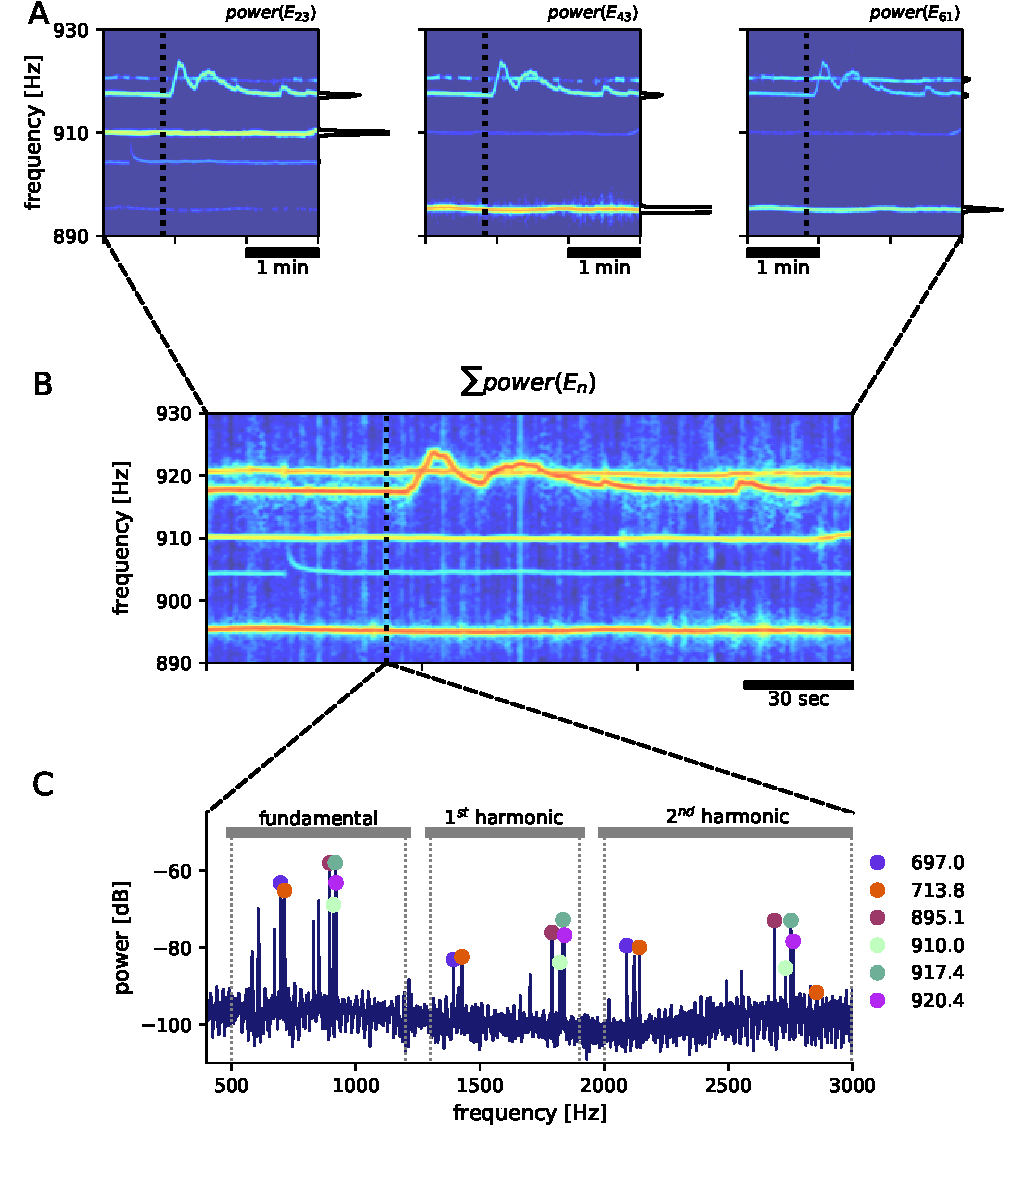
\includegraphics[width=.9\linewidth]{signal_extraction}}
%  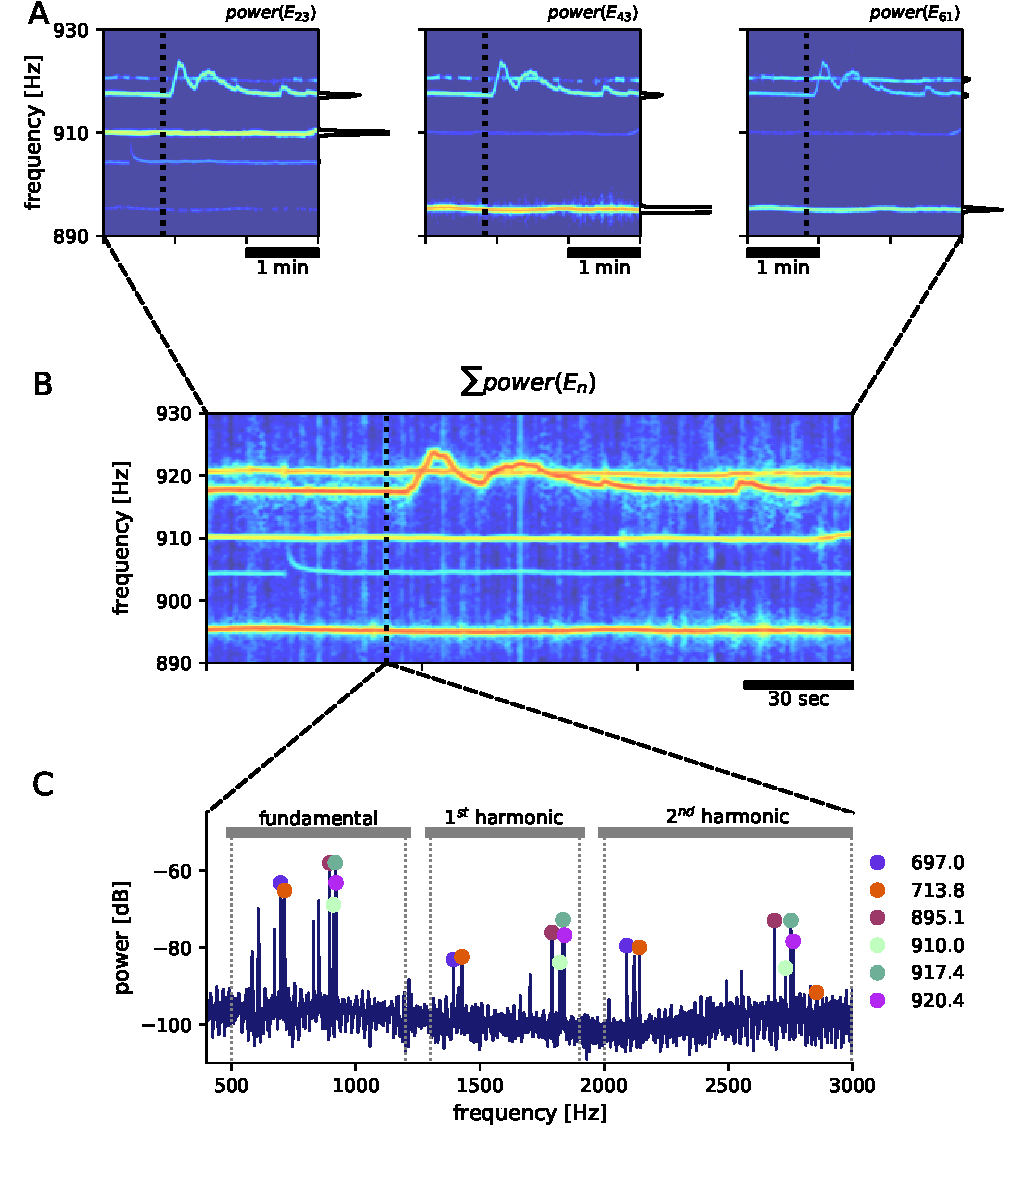
\includegraphics[scale=0.75]{signal_extraction}
  \caption{\label{signal_extraction} EOD frequency extraction from electric recordings obtained with an electrode array consisting of 8$\times$8 electrodes during the day of the 10$^{th}$ of April, 2016 in Colombia. \figitem{A} Spectrograms of a representative 3\,min  data snippet recorded on three example electrodes. Warmer colors represent increased power in respective frequencies. EODfs of individual \lepto{} remain rather stable, unless altered intentionally when emitting communication signals (see EODf trace starting at $\sim$~917\,Hz). A non-logarithmic PSD extracted at the time (50\,s) indicated with the dotted line is shown at the side of each panel. \figitem{B} By summing up spectrograms of all electrodes, more clear EODf traces can be obtained. \figitem{C} We detect frequency peaks in these summed up powerspectra and assign them into frequency groups corresponding to individual fish. A frequency group consists of an individual's fundamental EODf and at least two harmonics (see \citealp{Henninger2020}). Fundamental EODfs, their corresponding powers in the power spectra of all individual electrodes and their detection times are stored for the subsequent EODf tracking. } 
\end{figure}

%\subsection{Tracking wave-type electric fish signals}
\section{Tracking individual electric signals (EODs)}

For tracking individual EODs, we follow the approach of feature comparison. Previous approaches compare either EODf or signal power across electrodes over time \citep{Madhav2018, Henninger2020}. However, both of these signal features are time-variant and can potentially overlap between fish. EODf can be actively altered in the context of communication \citep{Smith2013} and the signal powers across electrodes change with the fish's motion \citep{Madhav2018}. This variability and potential overlap in signal features complicates reliable tracking, especially when fish are recorded in high abundance. Furthermore, existing algorithms tracking signals in order of their temporal detection, i.e. signals detected in consecutive time steps are assigned to already tracked EODf traces comprising preceding signals, potentially leads to tracking errors and accuracy limitations. Even with the utilization of an electrode array, EODs of freely moving and interacting electric fish are rarely detected continuously. Low signal-to-noise ratios, resulting from large distances between fish and recording electrodes or environmental conditions distorting electric fields, frequently lead to detection losses. When multiple fish with similar EODfs are recorded simultaneously, EODf traces can potentially cross each other (e.g. in the context of emitted communication signals, \citealp{Smith2013}). Especially in these occasions, detection losses can frequently result in tracking errors. 

In order to circumvent this issue, we developed a tracking algorithm which, first, uses a compound signal error including both differences in EODf and signal power across electrodes as tracking feature (\figref{features}) and, second, is less constrained by the temporal detection of signals (\figref{tmp_tracking}). 

\begin{figure}[h!]
  \centerline{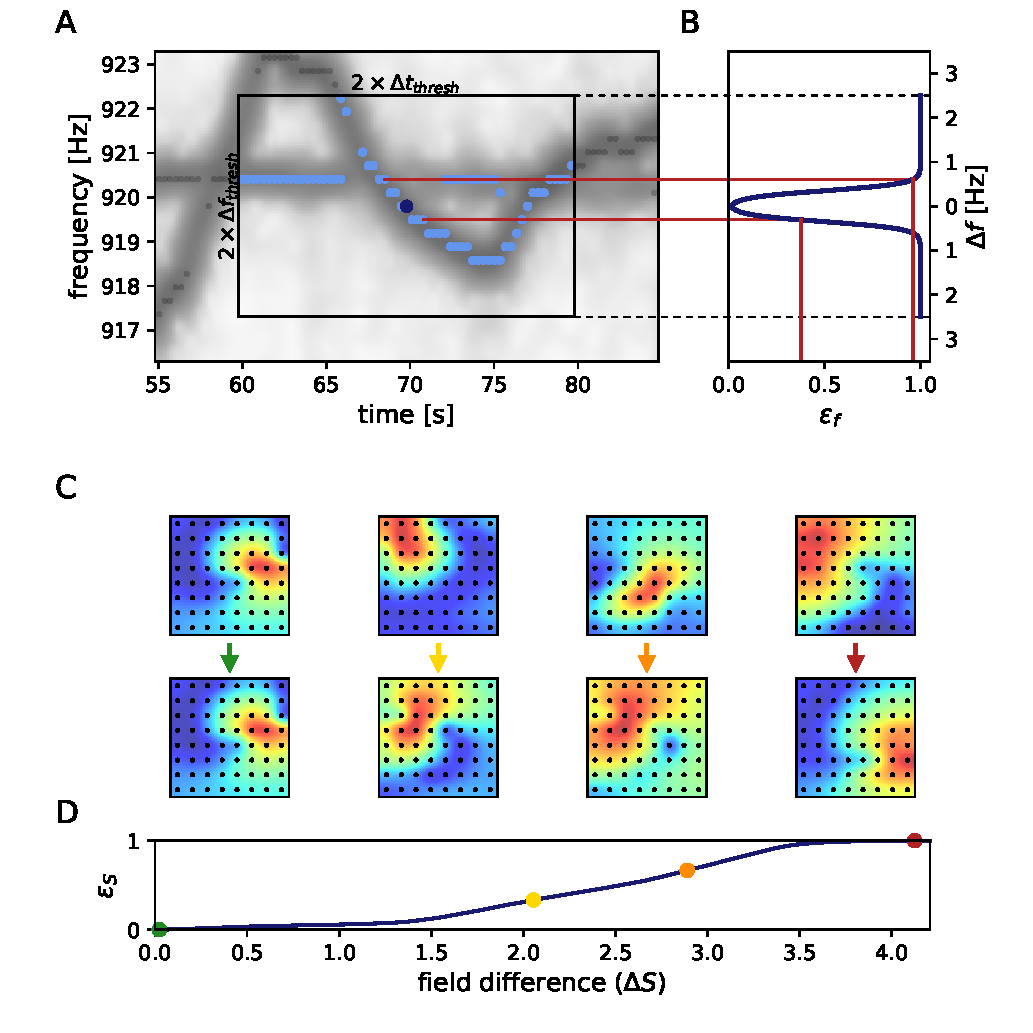
\includegraphics[width=.9\linewidth]{tracking_features_new}}
  \caption{\label{features} Signal errors are estimated to determine tracking order. \figitem{A} For each valid electric fish signal (see \figref{signal_extraction}), potential connection partners are limited by a time difference threshold ($\Delta t_{thresh}$) of $\pm$\,10\,s and a frequency difference threshold ($\Delta f_{thresh}$) of $\pm$\,2.5\,Hz. For a given signal (dark blue), potential connection candidates (light blue) need to be within these thresholds (box), whereas signals beyond these thresholds (grey dots) are rejected as potential connections. \figitem{B} Frequency differences are translated into frequency errors ($\varepsilon_{f}$) using a sigmoid function (\eqnrefb{errpr_eodf_eq}) favoring smaller frequency divergences. \figitem{C} The power distribution of a detected signal across all electrodes represents the basis for the second tracking parameter. The Euclidean distance of powers across electrodes between potential signal pairs (columns) represents the field difference ($\Delta S$, \eqnrefb{field_diff_eq}). With decreasing similarity (columns left to right) the field difference increases. \figitem{D} To obtain normalized field errors ($\varepsilon_{S}$) in the range of the frequency errors ($\varepsilon_{f}$), a given field difference is set into perspective to a representative distribution of field differences obtained by collecting all potential field differences of a manually selected 30\,s window in the recording.}
\end{figure}

\subsection{Identification of potential signal pairs}

The first fundamental assumption of the algorithm described below limits potential signal partners $\beta$ to a signal $\alpha$ by a maximal detection time difference of $\pm$10\,s and maximal EODf difference of $\pm$2.5\,Hz (\subfigref{features}{A}). To assess the similarity between each potential signal pair, we compare signal features ($\vec{X_{k, i}}$, \eqnrefb{signal_features}) by computing a signal error ($\varepsilon_{signal}$) as described below.

\subsubsection{Signal feature - EOD frequency}
As a first tracking feature we utilize the EODf difference 
\begin{equation}\label{f_difference}
\Delta f_{\alpha_i, \beta_j} = | f_{\alpha_i} - f_{\beta_j} |
\end{equation}
between signals with $f_{\alpha_i}$ as the EODf of signal $\alpha$ detected at time $i$ and $f_{\beta_j}$ of signal $\beta$ detected at time $j$ respectively. The EODf of electric fish represents one of the most stable natural oscillator known \citep{Moortgat1998} and has therefore already previously been used to track signals of electric fish \citep{Henninger2020}. Individual EODfs stay remarkably stable over a magnitude of minutes to hours. However, small fluctuations ($\leq$\,200\,mHz) can, first, occur naturally and, second, be an artifact of EODf detection in PSDs. Larger EODf differences, however, indicate either the occurrence of a (comparatively uncommon) communication signal (e.g. \citealp{Zupanc2002, Triefenbach2008, Raab2021}) or signals originating from different individuals. In order to adequately evaluate whether the EODf difference between a signal $\alpha$ and $\beta$ indicates them to originate from the same or different individuals, we compute a frequency error using a logistic function 
\begin{equation}\label{errpr_eodf_eq}   
  \varepsilon_{f}(\Delta f) = \frac{1}{1 + e^{-\frac{\Delta f - f_0}{df}}}
\end{equation}
with $\Delta f$ representing the EODf difference between the corresponding signals (\eqnrefb{f_difference}), $f_0 = 0.35$\,Hz being the frequency-offset and turning point of the logistic function, and $df = 0.08$\,Hz its corresponding slope (\subfigref{features}{B}). Applying this transformation, we mitigate the effect of small frequency differences ($\Delta f$) and equalize larger frequency differences in the assessment of whether two signals $\alpha$ and $\beta$ originate from the same or different individuals. 

\subsubsection{Signal feature - Electric field properties}

EODf traces of electric fish occasionally cross each other, e.g. when individuals actively alter their EODf in the context of communication (e.g. \citealp{Zupanc2002, Triefenbach2008, Raab2021}, \subfigrefb{features}{A}). Here, frequency as a tracking feature potentially results in flawed connections. Therefore, we utilize the spatial properties of a signal, i.e. signal powers across recording electrodes, as a complementary second tracking parameter reflecting the position and orientation of a fish (\citealp{Madhav2018}, \subfigrefb{features}{C}). The spatial properties 
\begin{equation}\label{field_properties}
S_{k, i}(x) = \frac{L_{k, i}(x) - L_{k, i_{min}}}{L_{k, i_{max}} - L_{k, i_{min}}}
\end{equation}
of a signal $k$ detected at time $i$ are the logarithmic signal powers ($L_{k, i}(x)$) extracted from the power spectrum of the respective electrode $x$ at the signal's frequency ($f_{k, i}$) normalized across recording electrodes by their smallest value 
\begin{equation}
L_{k, i_{min}} = \min_x L_{k, i}(x)
\end{equation}
and largest value ($L_{k, i_{max}}$) respectively. 

We compare the spatial properties of signals by computing their Euclidean distance 
\begin{equation}\label{field_diff_eq}
  \Delta S_{\alpha_i, \beta_j} = \sqrt{\sum_{x=1}^{n} (S_{\alpha_i}(x) - S_{\beta_j}(x))^2}
\end{equation} 
with $S_{\alpha_i}(x)$ and $S_{\beta_j}(x)$ being the normalized logarithmic powers extracted from the respective PSDs of electrodes $x$ at the frequencies $f_{\alpha_i}$ and $f_{\beta_j}$ of the respective signals  $\alpha_i$ and $\beta_j$. However, this arbitrary field difference ($\Delta S$) is heavily dependent on the configuration of the recording setup, especially on the number of recording electrodes used. To circumvent this issue and obtain field errors independent from the number of electrodes used in different recording setups, we define the field error 
\begin{equation}
\varepsilon_S(\Delta S_{\alpha_i, \beta_j}) = \int_0^{\Delta S_{\alpha_i, \beta_j}} p(\Delta S)\,d\Delta S
\end{equation}
 between the field properties $S_{\alpha_i}$ of signal $\alpha_i$ and $S_{\beta_j}$ of signal $\beta_j$ as the ratio of field differences in a representative field difference distribution ($p(\Delta S)$) smaller than the respective field difference to assess (\subfigref{features}{D}). To obtain this representative distribution of field differences ($p(\Delta S)$), we select a 30\,second data snippet within the respective data-set where fish can be assumed to be active (i.e. during night time) and compute the field differences for each potential signal pair ($\Delta t_{\alpha, \beta} \leq\pm$\,10\,s). 


\subsubsection{The compound signal error}

With the approach described above, we obtain for each signal pair a frequency error ($\varepsilon_{f}$) and field error ($\varepsilon_{S}$) ranging from 0 to 1. Finally, we compute the compound signal error ($\varepsilon_{signal}$) to quantify the overall disparity of signals using the formula
\begin{equation}\label{sig.error} 
  \varepsilon = \frac{2}{3} * \varepsilon_{S} + \frac{1}{3} * \varepsilon_{f}
\end{equation}
where we double weight the field error ($\varepsilon_{S}$) and single weight the frequency error ($\varepsilon_{f}$). This is because tracking issues usually arise from low $\varepsilon_{f}$. Nevertheless, $\varepsilon_{f}$ remains to be a relevant tracking feature, especially when fish are in close proximity (low $\varepsilon_{S}$).

\subsection{Snippet tracking}

\begin{figure}[t]
  \centerline{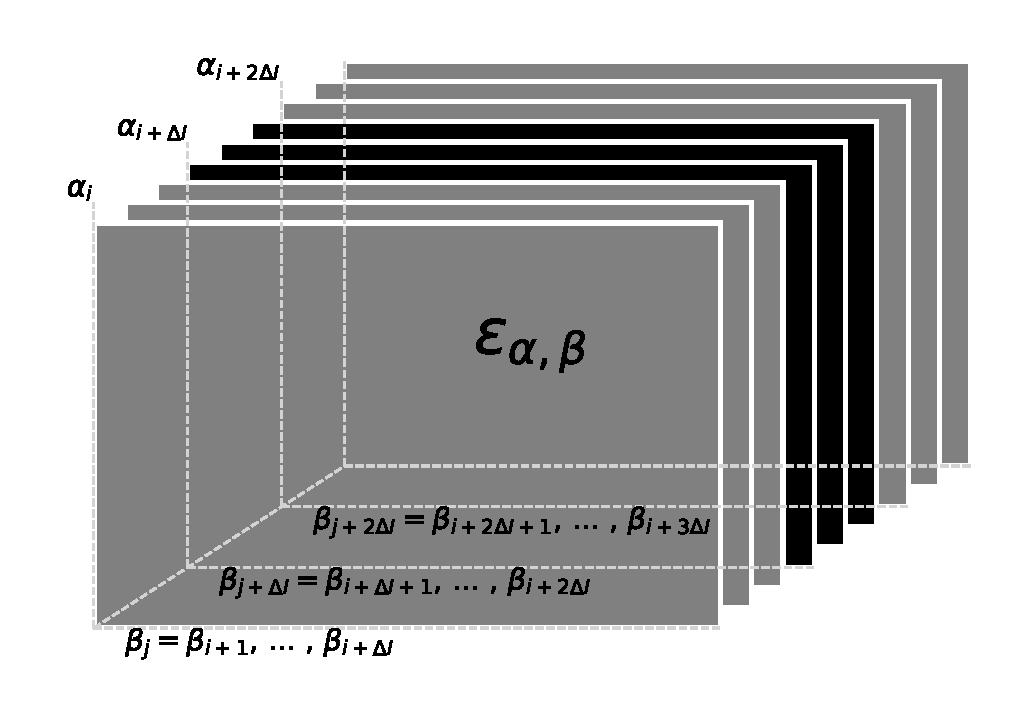
\includegraphics[width=.9\linewidth]{cube_error}}
  \caption{\label{error_cube} Error cube containing all signal errors ($\varepsilon_{\alpha, \beta}$) for possible signal pairs $\alpha$ and $\beta$ within the current tracking window. Each layer, referring to a time step $i$, contains the signal errors between all signals $\alpha_i$ detected at this time-step $i$ and their potential signal partners $\beta_j$ detected maximally 10\,s after signal $\alpha_i$ ($\Delta I$ time-steps after signal $\alpha_i$). Signal errors in grey layers correspond to signal pairs where one signal partner could potentially show a smaller signal error to a signal outside the error cube. Only connections based on the signal errors in the black layers can be assumed to be valid since all potential connections of both signal partners are within the error cube. Connections established in the 1$^{st}$ level tracking based on signal errors in black layers are appended to signal traces of previous tracking steps in the 2$^{nd}$ level tracking.}
\end{figure}

In order to reduce computation time and power without impairing tracking accuracy, we initially only track signals in snippets of 30\,seconds at a time (\figref{tmp_tracking}). Within these tracking windows, we first compute signal errors ($\varepsilon$) between each potential signal pair $\alpha$ and $\beta$ and store the corresponding signals errors in a three-dimensional error cube where the first two dimensions refer to signals $\alpha_i$ and $\beta_j$ and the third dimension to the time step $i$ where signals $\alpha_i$ have been detected (\figref{error_cube}). Connections between signal pairs are then established according to the order of signal errors stored in the error cube starting with the smallest 
\begin{equation}\label{min_e_signal_connect}
  \min \; \varepsilon_{\alpha, \beta}, \; \alpha \in \alpha_i,\;\dots,\;\alpha_{i + 2\Delta I}, \; \beta \in \beta_j,\;\dots,\;\beta_{j + 3\Delta I}, \; i \leq j \leq i + \Delta I  
\end{equation}
representing those signals $\alpha_i$ and $\beta_j$ most likely to originate from the same individual (\figref{tmp_tracking}). Depending on the signal pair and previously established connections, signal traces are established, appended, or joined. Connections are only valid and formed in the absence of temporal conflicts, i.e. a signal trace cannot feature two signals at the same time. As a result, we obtain signal traces build upon minimal signal errors within a 30\,seconds tracking window. 

However, since signals within the first and last 10\,seconds of a tracking window can potentially show lower signal errors to disregarded signals outside the current tracking window, these connections are potentially flawed (grey layers in \figref{error_cube}; grey bars in \figref{tmp_tracking}). Only connections established within the central 10\,seconds regard all other potential signal partners and can therefore be assumed to be valid. Accordingly, only the section of assembled signal traces corresponding to these central 10\,seconds of the current tracking window are further processed in the 2$^{nd}$ order tracking, where they are appended to already validated, previously detected signal traces (\figref{running_connection}). 

\begin{figure}[t]
  \begin{minipage}[t]{0.4\textwidth}\mbox{}\\[-2ex]
    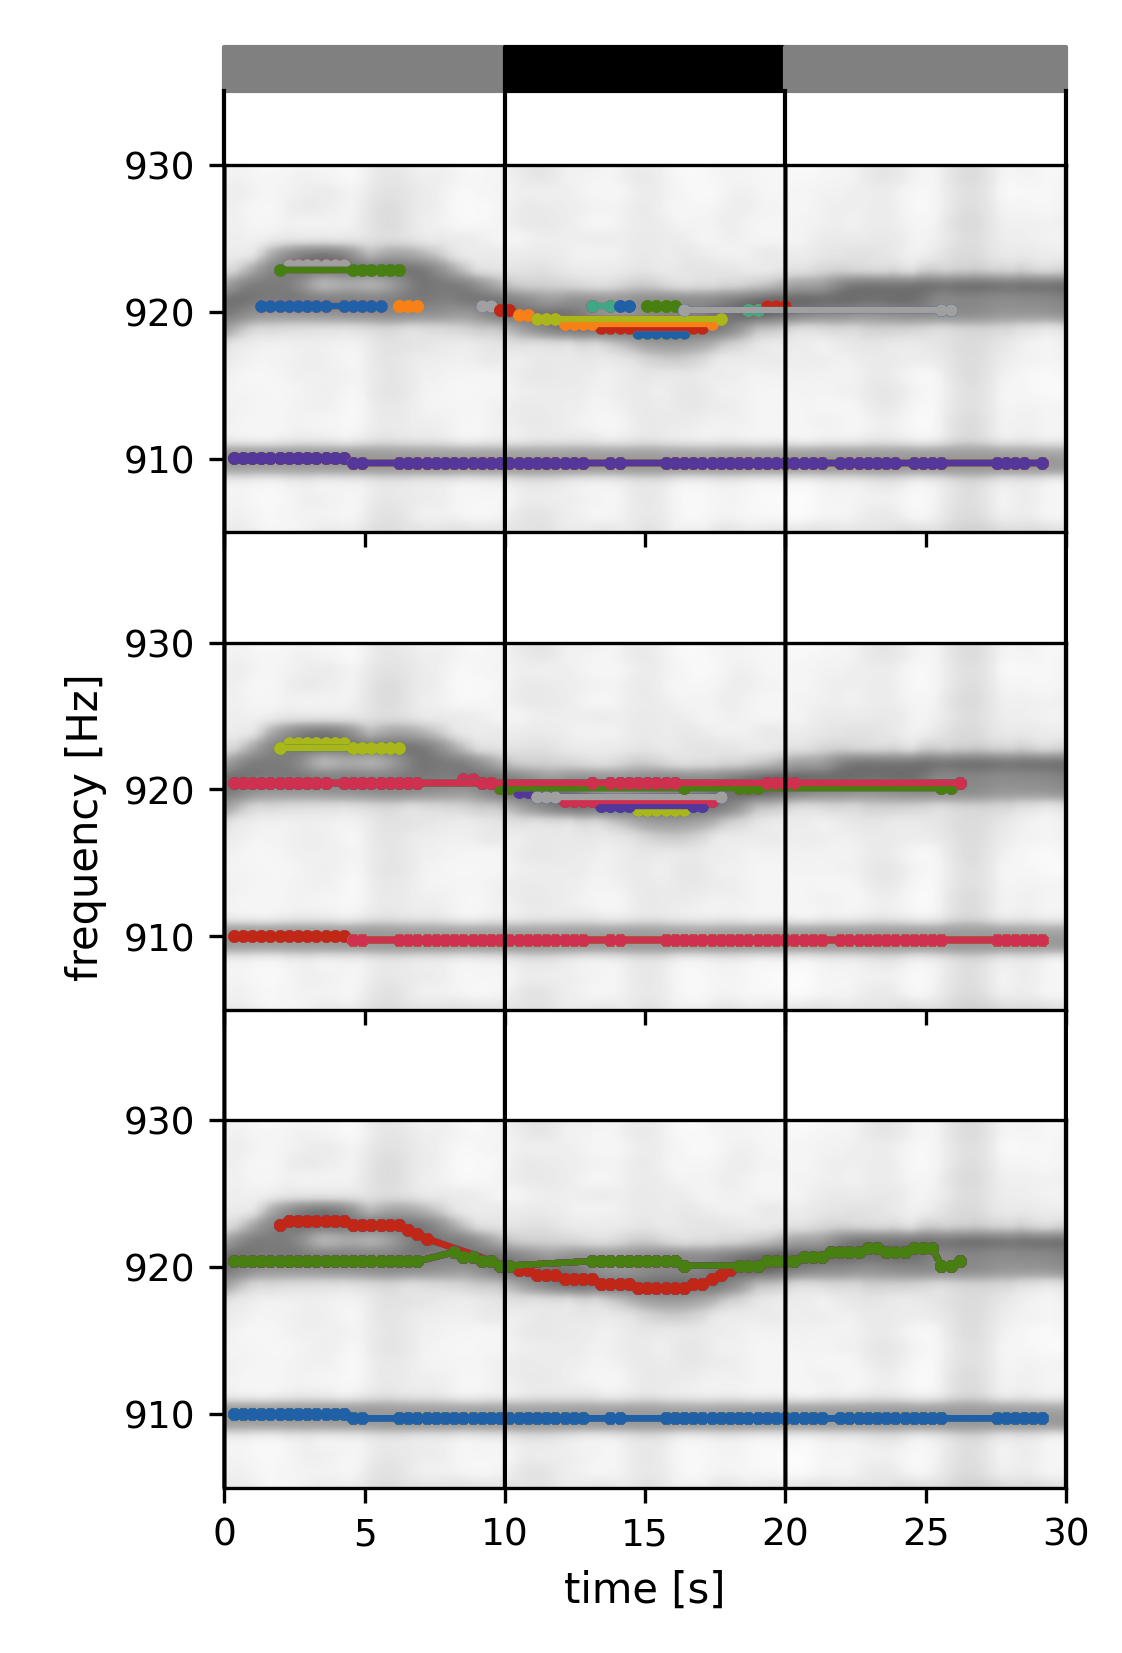
\includegraphics{tmp_ident_tracking}
  \end{minipage}
  \hfill
  \begin{minipage}[t]{0.38\textwidth}
  \caption{\label{tmp_tracking} 1$^{st}$ level signal tracking. Signals detected in  30\,s data snippets are connected to each other and assigned to fish identities according to their signal error. Signal pairs with smaller signal errors are connected first. With increasing signal error, more connections and identities are formed, complemented, or merged when no interference with already established connections emerge (no temporal overlap). Different stages of the 1$^{st}$ level tracking are shown in the three panels. While multiple separate signal traces are still present in the upper panels (different colors), only three EODf traces corresponding to three individual fish are left with the completion of the 1$^{st}$ level snippet tracking (bottom panel). Since each signal can potentially establish a best connection to a target signal in a range of $\pm$10\,s, only signal pairs within the central 10\,s of each 30\,s data snippet regarded all potential signal partners and are assumed to be valid. EODf traces in these central 10\,s are assigned to other EODf of previous tracking iterations.}
  \end{minipage}
\end{figure}

\subsection{Snippet assembly}
The assembly of the 10\,seconds signal traces obtained in the 1$^{st}$ level tracking (\subfigref{running_connection}{A}) and validated signal traces from preceding tracking steps (\subfigref{running_connection}{B}) proceeds, similar to the 1$^{st}$ order tracking, based on the smallest signal errors between them. 

To determine the connection order the smallest signal error 
\begin{equation}\label{min_e_snippet_connect}
  \min \; \varepsilon_{\alpha, \beta}, \; \alpha \in \alpha_i,\;\dots,\;\alpha_{i + \Delta I}, \; \beta \in \beta_{j + \Delta I},\;\dots,\;\beta_{j + 2\Delta I}, \; i \leq j \leq i + \Delta I 
\end{equation}
in the error cube between those signals $\alpha$ corresponding to the first 10\,seconds of the current tracking window ($\alpha \in \alpha_i \dots \alpha_{i + \Delta I}$) and signals $\beta$ referring to the central 10\,seconds of the current tracking window ($\beta \in \beta_{i + \Delta I} \dots \beta_{i + 2\Delta I}$) is determined. The 10\,second signal trace extracted in the 1$^{st}$ level tracking containing signal $\beta$ (green dot in \subfigref{running_connection}{C}), is then connected to the final  signal trace (from previous tracking steps) containing signal $\alpha$ (black dot in \subfigref{running_connection}{C}). This step is repeated with signal pairs of increasing signal errors until all possible connections are established (\subfigref{running_connection}{D}). 

The described 1$^{st}$ and 2$^{nd}$ order tracking steps are repeated alternately with data snippets shifted by 10\,seconds until the end of the recording is reached and tracking is finalized. For each tracking iteration, the error cube needs to be updated. Those layers referring to the time steps $i$ to $i + \Delta I$ of the first 10\,seconds of the previous tracking snippet are removed (frontal grey layers in \figrefb{error_cube}) and new layers referring to the next 10\,seconds beyond the last tracking snippet and their signal pairs $\alpha$ and $\beta$ are extended to the error cube in preparation for the next tracking iteration.


\begin{figure}[h!]
  \centerline{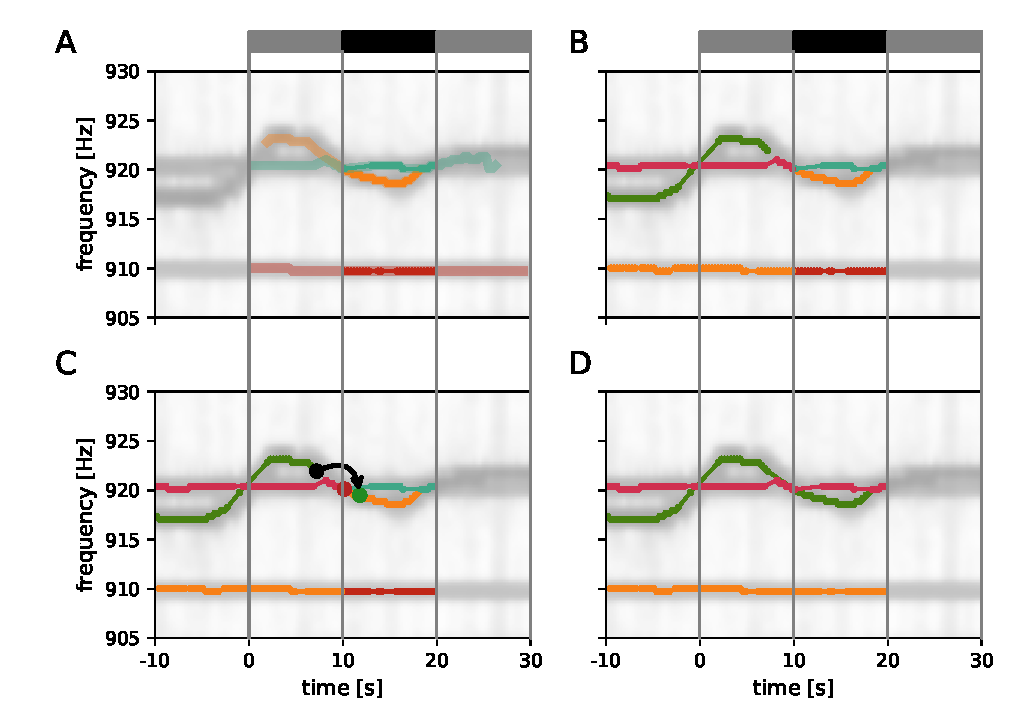
\includegraphics[width=.9\linewidth]{assign_tmp_identities}}
  \caption{\label{running_connection} 2$^{nd}$ level snippet tracking. EODf traces obtained from preceding 1$^{st}$ level tracking are connected to EODf traces of previous tracking steps. \figitem{A} EODf traces obtained from preceding 1$^{st}$ level signal tracking. Only connections within the central 10\,s of these EODf traces (opaque traces; black bar) can be assumed to be valid since signals before and after (faded traces; grey bars) have potential signal partners not accounted for in the 1$^{st}$ level signal tracking of the corresponding tracking window. \figitem{B} Additional display of EODf traces of previous tracking iterations. \figitem{C} EODf traces are connected according to the smallest possible signal error between any signal traces. The signal error between the origin signal (black) and the target signal (green) represents the smallest signal error between signal traces, which leads to the conjunction of the corresponding green and orange EODf traces. An alternative signal (red) has a larger signal error to the origin signal. \figitem{D} Connected EODf traces which will be extended in the next tracking iteration. }
\end{figure}

\subsection{Validation of signal traces}

Even though the developed algorithm is capable of tracking EODs of electric fish with unequalled accuracy (see below), occasional tracking errors still remain. We developed a GUI based software to visually inspect and validate tracked EODf traces and fix flawed connections (\figref{GUI}). Flawed connections can easily be identified by their clear deviation from the spectrogram displayed in the background. Furthermore, signal traces with a detection gap beyond the threshold of the tracking algorithm can be manually connected based on visual cues from the spectrogram. The resulting validated signal traces are then stored and analyzed depending on an experimental hypothesis \citep{Raab2019, Raab2021}.

\begin{figure}[h!]
  \centerline{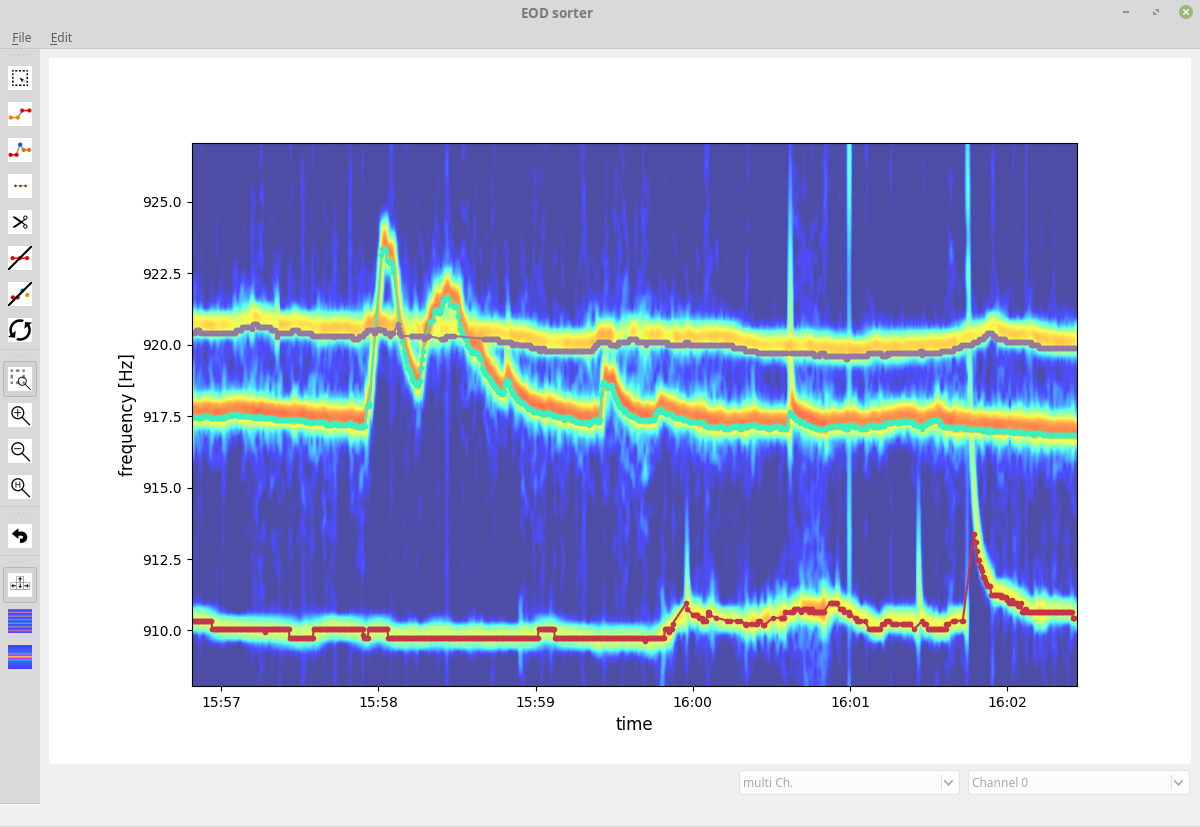
\includegraphics[width=.9\linewidth]{signal_tracker_GUI}}
  \caption{\label{GUI} Graphical user interface of the custom software developed to visually validate tracked signal traces and fix occasionally occurring flawed connections. The user is presented with the tracked signal traces (EODf traces) displayed on top of a summed up spectrogram, e.g. spectrograms added up across recording electrodes. The user can delete, cut, and connect signal traces or delete signals corresponding to electric noise.}
\end{figure}

\section{Detection and evaluation of tracking conflicts}

In order to quantify the accuracy of the presented tracking algorithm, we re-tracked signals of a whole population of \lepto{} recorded with an 8$\times$8 recording electrode grid in a small stream in the Llanos of Colombia during the day of 10$^{th}$ of April, 2016. During the tracking progress, connections established by the 1$^{st}$ level snippet tracking (\figref{tmp_tracking}) are compared to signal traces of the same recording after being visually inspected, corrected, and validated in post-processing using the GUI based Software (checked signal traces, \figref{GUI}). For each valid connection formed during the 1$^{st}$ level snippet tracking, i.e. when both signals $\alpha$ and $\beta$ are within the central 10\,seconds of the current tracking window, we determine whether a potential tracking conflict exists, e.g. if potential signal partners $\beta$ are associated with different checked signal traces. For each potential tracking conflict, we extract the EODf difference ($\Delta f$), field property difference ($\Delta S$), frequency error ($\varepsilon_f$), field error, ($\varepsilon_S$), and compound signal error ($\varepsilon$) between signal $\alpha$ and the best signal partner $\beta$ (smallest signal error $\varepsilon$) associated with the same checked signal traces (true connection), as well as between signal $\alpha$ and the best signal partner $\beta$ belonging to an alternative checked signal trace (false connection). 
%By comparing signal differences and error between true and false connections we are able to determine their suitability as tracking features (\figsref{signal_diff}, \fref{signal_error}).  

\section{Tracking feature quality assessment}

\begin{figure}[t]
  \begin{minipage}[t]{0.4\textwidth}\mbox{}\\[-2ex]
    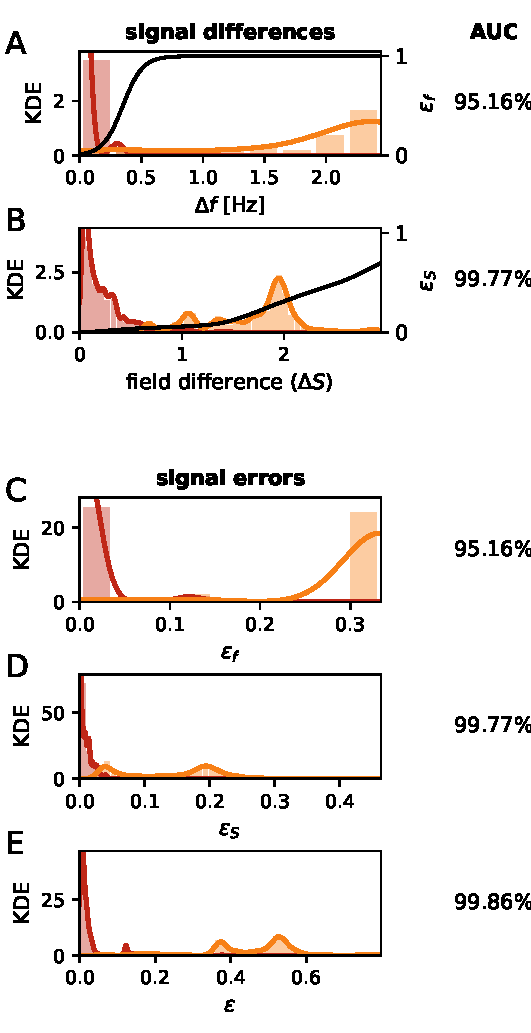
\includegraphics{signal_diff_error}
  \end{minipage}
  \hfill
  \begin{minipage}[t]{0.35\textwidth}
  \caption{\label{signal_diff_error} Often signals can potentially be assigned to multiple different signal traces of different fish (identified \textit{post hoc}). Smaller signal feature differences and errors to the origin signal indicate correct target signals (red). Signal differences and errors are larger for the alternative target signals (orange). \figitem{A} EODf differences are smaller to target signals than alternative signals. However, distributions overlap as quantified by a ROC-analysis (AUC$=$95.16\,\%). A sigmoid function (black) is used to translate EODf difference to frequency errors ($\varepsilon_{f}$). \figitem{B} Also field differences to target signals are smaller than to alternative signals. However, the overlap of corresponding distributions is smaller (AUC$=$99.77\,\%). The function translating field differences to field errors ($\varepsilon_{S}$) as described in \subfigref{features}{D} is shown in black. \figitem{C, D, E} Frequency error ($\varepsilon_{f}$, \panel~C), field error ($\varepsilon_{S}$, \panel~D), and compound signal error ($\varepsilon$, \panel~E) of origin signals to correct target signals (red) and alternative signals (orange). Frequency and field errors (C, D) resemble scaled signal differences (A, B) and are therefore equally suitable as tracking features (equal AUC). However, the compound signal error incorporating both field and frequency error is the most suitable for tracking electric fish signals and is therefore utilized in the presented algorithm (AUC$=$99.86\,\%).
  }
  \end{minipage}
\end{figure}

%\begin{figure}[h!]
%  \centerline{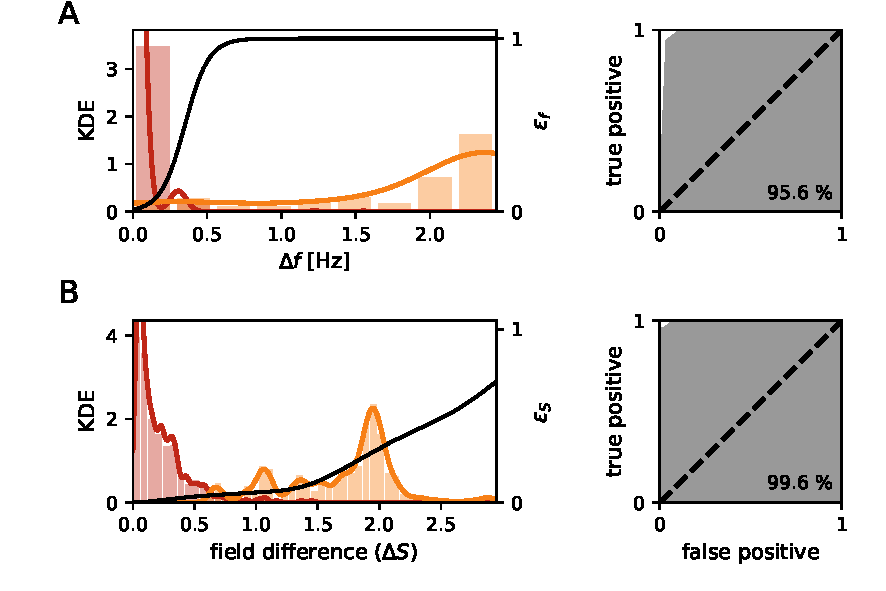
\includegraphics[width=.9\linewidth]{freq_field_difference}}
%  \caption{\label{signal_diff} Often a origin signal could potentially be assigned to signal traces originating from different fish (identified \textit{post hoc}). Different signal attribute differences vary depending on whether the origin signal is compared to the real, correct target signal (red) or the alternative potential signal partner (orange). \figitem{A} EODf difference are smaller to target signals before alternative signals. However, distributions overlap as quantified by a ROC-analysis (AUC$=$99.0\,\%, right panel). A sigmoid function (black) is used to translate EODf difference to frequency errors ($\varepsilon_{f}$). \figitem{B} Also field differences are smaller to target signals before alternative signals with a smaller overlap in distributions (AUC$=$99.6\,\%). The function translating field differences to field errors ($\varepsilon_{S}$) as described in \subfigref{features}{D} is shown in black.}
%\end{figure}

In order to assess the potential of each signal feature difference ($\Delta f$ \& $\Delta S$) and error ($\varepsilon_f$, $\varepsilon_S$, $\varepsilon$) to indicate true and false connections, we determine the area under the curve (AUC) of a receiver-operating characteristic between true and false connections as well as the proportion of signal differences/errors of true connections being smaller than those of the corresponding false connections (\figref{signal_diff_error}). While tracking a full data-set recorded during the day of the 10$^{th}$ of April, 2016, $261\,344$ potential tracking conflicts were detected and are evaluated in the following. To highlight the capabilities of the presented tracking algorithm, we first evaluate only those tracking conflicts corresponding to a 5\,minute snippet being especially challenging to track because of several crossing EODf traces. A representative segment of this 5\,minute data snippet is displayed in \figref{GUI} and is the basis for \figsref{signal_extraction}, \fref{features}, \fref{tmp_tracking} and \fref{running_connection}

The least reliable tracking feature appears to be an individual's EODf ($\Delta f$/$\varepsilon_f$). Regarding only tracking conflicts corresponding to the challenging to track 5\,minute data snippet, frequency differences/errors of true connections were smaller in only 94.83\,\% (440/464) of the cases and the comparison of frequency difference/error distributions between true and false connections using a ROC-analysis resulted in an AUC of 95.16\,\% (\subfigref{signal_diff_error}{A, C}). Better results can be achieved utilizing the field property differences ($\Delta S$/$\varepsilon_S$) as tracking feature. For the tracking conflicts corresponding to the challenging to track 5\,minute data snippet, field property differences of true connections were smaller in 99.57\,\% (462/464) of the cases and the AUC from the ROC-analysis describing the difference between the distributions of field differences/errors between true and false connections already reached 99.77\,\% (\subfigref{signal_diff_error}{B, D}). However, these results can even be surpassed when utilizing a compound signal error ($\varepsilon$) combing both frequency error ($\varepsilon_f$) and field error ($\varepsilon_S$). In 99.87\,\% (462/464) of the tracking conflict corresponding to the 5\,minute data snippet, true connections had smaller compound signal error ($\varepsilon$) than false connections. The associated ROC-analysis evaluating the difference between signals errors of true and false connections resulted in an AUC of 99.86\,\% (\subfigref{signal_diff_error}{E}). 

Regarding all tracking conflicts of the whole recording, similar observations could be made. However, the higher proportion of ``easy'' tracking conflicts led to a shift of tracking feature accuracy to higher values and differences between them were less pronounced. Nevertheless, EODf still remained to be the least favorable tracking parameter (99.73\,\% smaller frequency errors in true connections than in false connections; AUC = 99.79\,\%) followed by the field difference (99.81\,\% smaller frequency errors in true connections than in false connections; AUC = 99.85\,\%). The best results could be achieved when utilizing the compound signal error for tracking (99.95\,\% smaller frequency errors in true connections than in false connections; AUC = 99.98\,\%).


\section{The advantages of the presented algorithm}

Previous approaches on tracking EODs of individual wave-type electric fish either utilized their EODf \citep{Henninger2020} or the spatial properties of their electric fields \citep{Madhav2018} as tracking features. We assessed how suitable both signal features alone  as well as a combination of both (compound signal error: $\varepsilon$, \eqnrefb{sig.error}) are for tracking by evaluating tracking conflicts occurring while processing a recording of a natural, high density population of \lepto{} in a stream in Colombia. 

According to this evaluation, the comparison of spatial field properties ($\Delta S$) achieves a higher tracking accuracy than EODf comparison ($\Delta f$). Certainly, the EODf of \lepto{} can be remarkably stable over minutes to hours \citep{Moortgat1998}. However, \lepto{} frequently alters its EODf actively in the context of electrocommunication \citep{Smith2013}. Accordingly, the suitability of EODf as tracking feature decreases the more fish are recorded and analyzed simultaneously since EODf differences between fish are potentially smaller and interactions between fish involving active EODf alterations can be assumed to be more frequent. Therefore, spatial field properties resembling a fish's spatial position and orientation represent a more honest and suitable tracking feature, especially when only those signal pairs with small EODf differences ($\Delta f$) are regarded for comparison and tracking.

Nevertheless, the highest tracking accuracy can be achieved by utilizing a compound signal error ($\varepsilon$) comprising both EODf difference ($\Delta f$) and spatial field property difference ($\Delta S$) as tracking feature. This is because the compound signal error ($\varepsilon$) implements a tracking bias that helps to resolve tracking conflicts in the event of crossing EODf traces. In such intersections, temporarily only one signal can be extracted by detecting peaks in the compound PSD (e.g. \subfigref{features}{A}). Since the spatial properties ($S$) of these overlaid signals comprise the electric field properties of both individual signals, their assignments are only correct at chance level when solely the signals' spatial field properties are utilized for tracking. The compound signal error ($\varepsilon$), on the other hand, slightly favors connections of signal pairs with more similar EODfs resulting in a bias for overlaid signals detected in EODf trace interactions to be connected to the EODf traces of those fish not altering their EODf (\figref{tmp_tracking}, green trace in bottom panel). The other signal traces, accordingly, remain to be connected across the intersection afterwards. 

The advantage of the presented tracking algorithm not only rests upon the utilization of a compound signal error as tracking feature, but also on the tracking method itself. When studying animals and their behaviors by means of evaluating external recordings, we rely on the detection of sensory cues emitted actively or passively by the animals themselves \citep{Dell2014, Hughey2018}. In cluttered environments or when signals are weak (low signal-to-noise-ratio), reliable signal detection is often impaired and detection losses frequently occur. These detection gaps complicate reliable tracking, especially when signals are tracked according to their temporal occurrence. In recordings of electric fish, detection losses frequently result from fish being too far away from recording electrodes or electric field being blocked by any objects between fish and recording electrode. However, associated tracking issues can be avoided with the presented algorithm since it is less reliant on the temporal detection of signals, but connections are rather established according to the smallest signal errors in discrete tracking windows.

\section{Conclusion}

The electric field of \lepto{} poses a great opportunity for studying natural behaviors of electric fish in freely moving and interacting populations. The EODs of whole groups can be recorded simultaneously by means of recording electrode arrays submerged in the water and tracked for individual fish using different EOD characteristics. With the presented algorithm, we combine previous approaches of tracking either the individual specific EODf \citep{Henninger2020} or the spatial properties of electric fields resembling a fish's spatial location and orientation \citep{Madhav2018}. We use a compound signal error incorporating both EODf and spatial field property difference and obtain EOD traces of individual fish by assembling signals in discrete tracking windows according to the order of increasing signal errors. With this approach, our algorithm improves in resolving various tracking issues, e.g. resulting from crossing EODf traces or detection losses, and enables EOD tracking with unprecedented accuracy. Since tracked EOD traces allow insights into various behavioral aspects of electric fish, including communication and movement, our algorithm is applicable in a broad range of behavioral studies. It also facilitates high throughput studies including long term behavioral observation since the increased tracking accuracy decreases the expense of extensive EOD trace post-processing. This has already been demonstrated in an experiment evaluating the spatio-temporal movements of a group of 14 \lepto{} in the context of an individual's social status \citep{Raab2019} as well as in an experiment investigating the communication behavior of pairs of \lepto{} competing over a shelter during staged competition \citep{Raab2021}.
%\bibliography{journalsabbrv,references}
%\figurecaptions

%\bibliographystyle{jneurosci}
%\bibliography{../journalsabbrv,../references}



\cleardoublepage
\graphicspath{{chapter_3_habitats/figures/}}
%\chapter{\mbox{Habitat preference and explorative behavior}}
\chapter{\mbox{Group dispersion and movement patterns}}
\label{Habitats}

\textbf{The literal content of this chapter has already been published as:}\\  
Till Raab, Laura Linhart, Anna Wurm, Jan Benda (2019) Dominance in Habitat Preference and Diurnal Explorative Behavior of the Weakly Electric Fish \Lepto{}. \textit{Frontiers in Integrative Neuroscience} 13:21.

\paragraph*{Contributions}
For this scientific project Till Raab designed the experiments, collected and analyzed the data, performed post-processing of electric EOD recordings, generated the displayed figures, and wrote the manuscript. 
Laura Linhart and Anna Wurm collected the data and performed post-processing of electric EOD recordings while being supervised by Till Raab. Laura Linhart additionally provided the sketches of the experimental tank displayed in \subfigref{eodtraces}{A, B}. 
Jan Benda discussed the experiments, advised data analysis, and assisted writing the manuscript. 

%\section{Abstract}
\begin{quote}
\begin{center}
\large\textbf{Abstract}
\end{center}
Electrocommunication and -localization behaviors of weakly electric fish have been
studied extensively in the lab, mostly by means of short-term observations on constrained
fish. Far less is known about their behaviors in more natural-like settings, where fish
are less constrained in space and time. We tracked individual fish in a population of
fourteen brown ghost knifefish (\Lepto{}) housed in a large 2\,m$^3$ indoor
tank based on their electric organ discharges (EOD). The tank contained four different
natural-like microhabitats (gravel, plants, isolated stones, stacked stones). In particular during the day individual fish showed preferences for specific habitats which provided appropriate shelter. Male fish with higher EOD frequencies spent more time in their preferred habitat during the day, moved more often between habitats during the night, and less often during the day in comparison to low-frequency males. Our data thus
revealed a link between dominance indicated by higher EOD frequency, territoriality, and
a more explorative personality in male \lepto{}. In females, movement activity
during both day and night correlated positively with EOD frequency. In the night, fish
of either sex moved to another habitat after about 6\,s on average. During the day, the
average transition time was also very short at about 20\,s. However, these activity phases
were interrupted by phases of inactivity that lasted on average about 20\,min during the
day, but only 3\,min in the night. The individual preference for daytime retreat sites did not reflect the frequent explorative movements at night.
\end{quote}
\hfill

\section{Introduction}
Weakly electric fish are nocturnally active. In the night, many pulse-type fish increase the
rate of their electric organ discharges (EOD) \citep{Lissmann1965,Stoddard2007}, wave-type fish emit various kinds of electrocommunication signals more frequently \citep{Zupanc2001,Henninger2018}, and gymnotids have been shown to move from deep waters up to the shore \citep{Steinbach1970}. During the day, weakly electric fish hide under submerged logs (\textit{Gymnotus}, \citealp{Westby1988}), between roots (\textit{Eigenmannia}, \citealp{Hopkins1974}), in leaf litter (\textit{Brachyhypopomus}, \citealp{Hagedorn1988}), or bury themselves in sand (\textit{Gymnorhamphichthys}, \citealp{Lissmann1965}).

EOD frequencies of the gymnotiform brown ghost knifefish \lepto{} are sexually dimorphic with males having higher EOD frequencies than females \citep{Meyer1987}. In playback experiments with restrained fish, males more frequently produced aggressive communication signals (chirps) than females \citep{ZupancMaler1993, Bastian2001} and in experiments of free swimming fish, male \lepto{} showed a higher overall chirp rate compared to females \citep{Dunlap2002,Hupe2008}. However, during courtship in the field females produced almost as many chirps as males \citep{Henninger2018}, and both sexes jammed rivals by approaching their EOD frequencies \citep{Tallarovic2002}. In competition experiments, male \lepto{} were
more likely to inhabit tubes alone, whereas females cohabited tubes more often \citep{Dunlap2002}.

Several studies suggest higher EOD frequencies in males as an indicator of dominance. Additionally, body size correlated with EOD frequency in males \citep{Triefenbach2008, Fugere2011} but not in females \citep{Dunlap2002}. Dominant males with higher EOD frequencies were more aggressive \citep{Fugere2011} and participated more in mating
\citep{Hagedorn1985, Henninger2018}. In competition experiments, males with higher EOD frequencies occupied the most preferred tubes, whereas females did not distribute according to EOD frequency \citep{Dunlap2002}. In summary, these laboratory studies suggest that male
brown ghost knifefish are territorial at their preferred retreat site during the day, and that males with higher EOD frequencies are more dominant.

Observations on aggression and dominance have previously been limited to studies in the lab in small tanks, and mostly to short observation times (e.g., \citealp{Hopkins1974, Hagedorn1985, Nelson1999, Tallarovic2005, Triefenbach2008, Hupe2008}). Recent technological advances allow for long-term observations of electric activity of these fish in the lab and in the field \citep{Henninger2018, Madhav2018}. Here, we take advantage of these methods and describe diurnal activity patterns of a community of \lepto{} competing for different
microhabitats in a large indoor tank over 10 days.

\section{Methods}
Six male and eight female \lepto{}, obtained from a tropical fish supplier, were housed in a $2.5 \times 1 \times 0.8$\,\cubic\meter{} indoor tank with a water conductivity of 320\,\micro\siemens\per\centi\meter{} at a 12\,h/12\,h light cycle. Initially, four fish inhabited the tank. Starting at day 4 we introduced two additional fish per day. Fish were selected for approximately equal size to minimize effects based on physical differences as far as possible. All fish were mature and not in breeding condition. EOD frequency is sexually dimorphic in \lepto{} \citep{Meyer1987}. We identified fish with EOD frequencies lower than 750\,Hz as females, and fish with higher EOD frequencies as males \citep{Henninger2018}. Four natural-like habitats in $60 \times 45 \times 10$\,\centi\meter\cubed{}  PVC-containers were arranged next to each other in the tank: stacked stones, quartz gravel (few millimeters diameter), isolated stones, and aquatic plants (\textit{Vallisneria spec.}) (\subfigrefb{eodtraces}{A}). Fish were fed frozen \textit{Chironomus plumosus} on the gravel habitat every day at about 8\,h after lights were switched on. Animal housing complied with national and European law and was approved by the
Regierungspr\"asidium T\"ubingen (permit no: 35/9185.46/UniT\"U). Approval by an ethics committee was not required because our study was purely observational.

We continuously recorded EODs for 10 days and nights using 16 monopolar electrodes at low-noise headstages, and digitized at 20 kHz per channel with 16 bit resolution (see \citealp{Henninger2018} for details). For each of the four habitats, two electrodes were placed at the bottom of the habitat 35\,cm apart and two electrodes 35\,cm above the respective electrodes in the habitats in the open water (\subfigrefb{eodtraces}{A, B}). Water temperature was measured once a day. During the course of the experiment, water temperature steadily dropped from 26.3\,\celsius{} to 24.8\,\celsius. Fish were identified by their specific peaks in the spectrogram of the recordings (nfft = $2^{16}$, overlap = 90\,\%) and tracked using a custom tracking algorithm comparing fundamental EOD frequency and the corresponding power pattern in the spectrograms of the different electrodes (see \citealp{Henninger2018} and \citealp{Madhav2018} for details).

Every 0.328\,ms (temporal resolution of the spectrogram), fish were assigned to habitats by means of the electrode with the largest power at the fish's EOD frequency. Based on this spatial information we analyzed how the fish occupied the habitats. For each day and night, we computed the fraction of fish in each habitat by dividing the detections within one habitat by the total number of detections on that day or night (\subfigref{eodtraces}{E}). Likewise, individual habitat preferences were computed separately based on the detections of each fish (\subfigref{habitatpref}{A}). To assess the number and composition of fish in each habitat we counted the number of males and females detected in each habitat for every time
step (\subfigref{habitatpref}{C}). The male ratio is the number of males in a habitat divided by the total number of detected fish in that habitat (\subfigref{habitatpref}{D}).

The preferred habitat of a fish was defined as the habitat where the fish spent most of the time, i.e., had the most detections, for each day and night. Relative time spent in the preferred habitat was computed as the ratio between detections in the preferred habitat and the number of detections per day or night (12\,h $\times$ 3600\,s/h $\times$ 3.05 detections per second $\approx$ 131,827 detections per 12\,h) for every day and night (\subfigref{habitatpref}{B}). The stability of individual habitat preferences was evaluated using preference change rates, i.e., the probability of a fish to change its preferred habitat from one day or night to another one, computed as the number of days (or nights) on which the fish preferred a different habitat as on the previous day (or night) divided by the number of days the fish was in the tank minus one (\subfigref{transitions}{A, C}).

Transitions of fish between habitats were characterized by the number of transitions of detections from electrodes of one habitat to electrodes from another habitat (\subfigref{transitions}{B, D}). The distributions of transition times $\Delta t$, i.e., the time spans a fish spent in one habitat between two habitat changes, were exponentially distributed (\subfigref{transitiontimes}{A}):
\begin{linenomath}
  \begin{equation}
    \label{expdist}
    p(\Delta t) = \lambda e^{-\lambda \Delta t} \; .
  \end{equation}
\end{linenomath}
The number of transitions per time (\subfigrefb{transitions}{B}) is the
transition rate. In \subfigref{transitiontimes}{B} the transition rate
$\lambda=1/\tau$ was estimated from the average transition time $\tau
= \frac{1}{n} \sum_{i=1}^n \Delta t_i$ for each fish separately for
days and nights.

The tails in the distributions of transition times dominate the activity patterns of the fish because a single long transition time implies a non-moving fish for exactly this time. During the same time, however, many more short transitions can occur. Short transition times are thus overrepresented when taking the average.  To account for this we also computed a weighted average $\overline{\Delta t_i}$, where we weighted each transition time $\Delta t_i$ by its duration $\Delta t_i$ (\subfigref{transitiontimes}{C}):
\begin{linenomath}
  \begin{equation}
    \label{weightedtime}
    \overline{\Delta t_i} = \frac{\sum_{i=1}^n \Delta t_i^2}{\sum_{i=1}^n \Delta t_i}
  \end{equation}
\end{linenomath}

Finally, we investigated if individual habitat changes were independent of each other by calculating the time differences between a fish entering a habitat and the other fish leaving the respective habitat. We compared these distributions to boot strapped distributions where entering times to a random habitat were set randomly throughout the whole recording period.

Because fish were in similar physical condition and their sexes were determined using only a hard EOD frequency cutoff at 750\,Hz we performed a sensitivity analysis for all corresponding results, i.e., additionally to the original sex assignments, all
statistics were calculated with up to $\pm 2$ males or females, where the individuals closest to the cutoff were assigned to the opposite sex.

For quantifying differences between groups, we used Cohen's $d$ for unequal group sizes:
\begin{linenomath}
  \begin{equation}
    \label{cohensd}
    d = \left| \frac{\mu_1 - \mu_2}{  \frac{n-1}{n+m-2} \sigma_1^2  +   \frac{m-1}{n+m-2} \sigma_2^2    }    \right|
  \end{equation}
\end{linenomath}
where $\mu_1$ and $\mu_2$ are the means, $\sigma_1$ and $\sigma_2$ the standard deviations, and $n$ and $m$ the group sizes, respectively.

\section{Results}

We observed the movements of six male and eight female \lepto{} between four microhabitats and the open water in a two cubic meter tank over 10 days. We tracked individual fish
based on EOD frequency and power on 16 recording electrodes (\subfigrefb{eodtraces}{C}). EOD frequency is known to be sexually dimorphic in \lepto{} \citep{Meyer1987}. Fish with an EOD
frequency above 750\,Hz are defined as males, fish below 750\,Hz as females (\subfigrefb{eodtraces}{D}, \citealp{Henninger2018}). The overall decline of EOD frequencies followed the water temperature, which decreased by 1.5\,\celsius{} over the course of the experiment. In fact, the $Q_{10}$ values computed for each fish from daily temperature
measurements and the corresponding EOD frequencies (median $Q_{10}=1.54$) were close to typical $Q_{10}$ values reported for these fish in the literature \citep{Dunlap2000, Stoeckel2014}. Additionally, circadian modulations of each fish's EOD frequency followed similar patterns and can also be best explained by periodic diurnal water temperature changes \citep{Dunlap2000}. On top of these exogenous influences, the fish actively changed
their EOD frequency, approaching and evading EOD frequencies of other fish. For example, the EOD frequencies of the males indicated in orange and blue approached each other and got
closer to the males indicated in red and green. Female fish also approached each other in their EOD frequency and even switched order (e.g., the females indicated in red and light blue at the bottom of \subfigrefb{eodtraces}{C}). In the following we do not analyze
these modulations of EOD frequency but rather focus on diurnal movement patterns.

\begin{figure*}[p]
  \showfigure{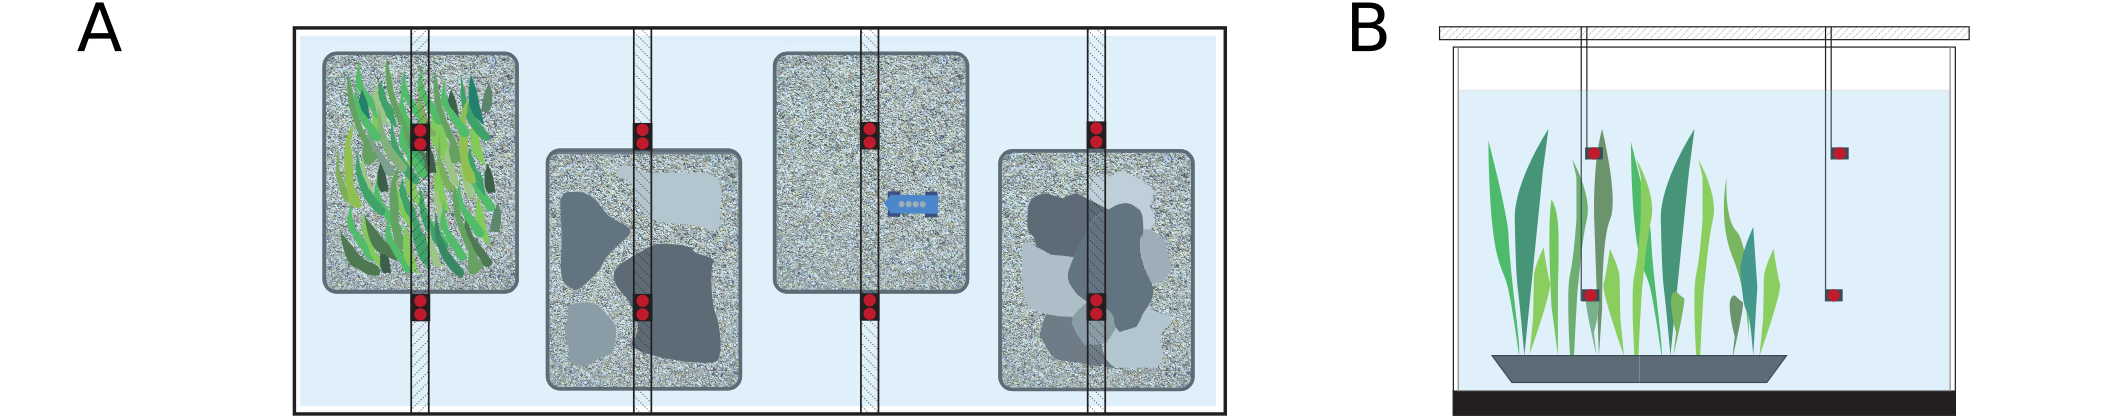
\includegraphics[width=1\linewidth]{habitats.png}\\[3ex]
    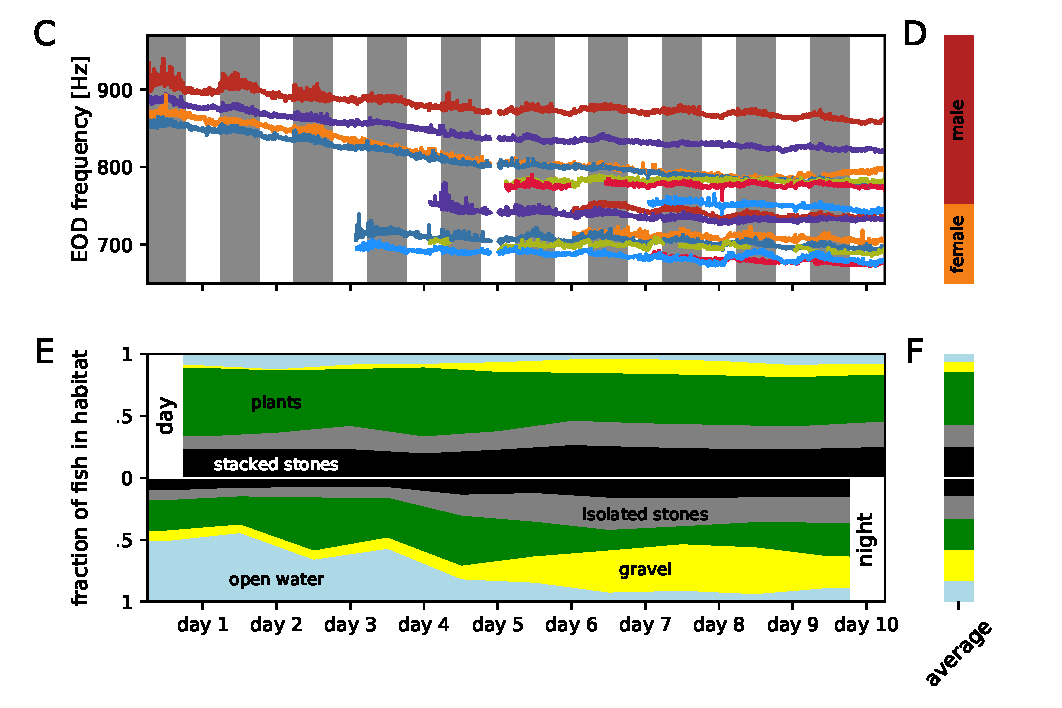
\includegraphics[width=1\linewidth]{traces_distribution}}
  \caption{\label{eodtraces} Experimental setup, EOD frequencies and
    distribution of fish over habitats. \figitem{A} Top view of the
    experimental setup with four different micro habitats (plants,
    isolated stones, gravel, stacked stones). Electrodes (red) were
    fixed in location by PVC poles positioned above the tank. Fish
    were fed on a daily basis on the gravel habitat using a custom PCV
    feeder (blue). \figitem{B} Side view of the experimental setup
    showing the electrodes positioned in two levels over the
    habitats. \figitem{C} EOD frequency traces tracked over the entire
    duration of the experiment. Individual fish are marked by the same
    color in all figures. \figitem{D} Ranges of male (red) and female
    (orange) EOD frequencies. \figitem{E} Fraction of fish detected
    within each of the five habitats for consecutive days (top) and
    nights (bottom). \figitem{F} Relative occupation of the habitats
    averaged over all days (top) and nights (bottom).}
\end{figure*}

\subsection{Habitat occupation}
The tank offered the fish four different 0.25\,m$^{2}$ habitats that contained either stacked stones, quartz gravel, isolated stones, or aquatic plants. We counted the open water above the habitats as a fifth habitat. For each time point we assigned each fish to one of
these habitats according to the electrode with the largest power at its EOD frequency.

During the days, i.e., the presumably inactive phases of the fish, most fish were located within the aquatic plants followed by the stacked stones and the isolated stones. Fish were rarely found in the gravel habitat or in the open water (\subfigrefb{eodtraces}{E, F}, top). At night, no habitat seemed to be preferred on average (\subfigrefb{eodtraces}{E, F}, bottom).

During the days, the addition of fish did not influence the distribution of fish in the habitats by a lot (\subfigrefb{eodtraces}{E}, top). The standard deviation of the fraction of fish occupying a habitat was below 6.5\,\% for all habitats. Nevertheless, the fraction of fish occupying isolated stones or gravel increased slightly throughout the experiment (Spearman's rank correlation: $r=0.76$, $p=0.005$ and $r=0.88$, $p<0.001$, respectively), whereas the occupation of the aquatic plants and the open water slightly decreased within
the 10 days (Spearman's rank correlation: $r=-0.76$, $p<0.05$ and $r=-0.65$, $p<0.05$, respectively). The occupation of the stacked stones habitat was unaffected by the increasing
fish count and did not change over the days of the experiment (Spearman's rank correlation: $r=0.37$, $p=0.30$). Consequently, the increasing total fish count led to an almost uniform increase in the number of fish occupying each habitat. None of the habitats was claimed exclusively by a dominant fish as a retreat site during the days.

In contrast, at nights the increased fish count seemed to influence the distribution of the fish over the habitats more strongly (\subfigrefb{eodtraces}{E}, bottom). The occupation of both the isolated and stacked stones habitats increased slightly during the course of the experiment (Spearman's rank correlation: $r=0.84$, $p<0.01$ and $r=0.79$, $p<0.01$, respectively), whereas the fraction of fish in the open water clearly decreased (Spearman's rank correlation: $r=-0.90$, $p<0.001$) and the occupation of the gravel habitat increased (Spearman's rank correlation: $r=0.95$, $p<0.001$). The latter could be attributed to the experimental design. Food was supplied daily at the gravel habitat and gymnotiform fish
have been shown to learn the location of food \citep{Jun2013}.

\begin{figure*}[t!]
  \showfigure{\centerline{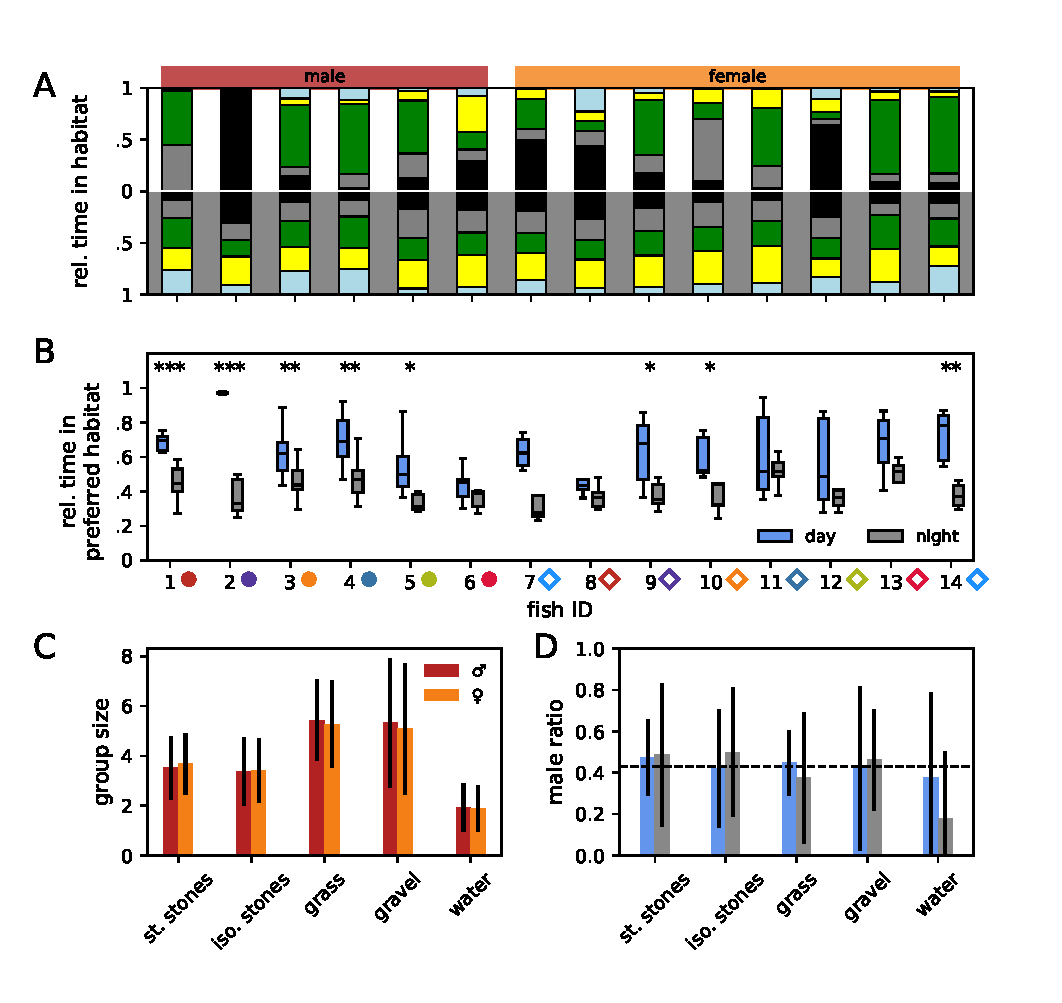
\includegraphics[width=1\linewidth]{habitat_pref}}}
  \caption{\label{habitatpref} Habitat preference.
    \figitem{A} Relative time each individual fish spent in the
    different habitats (same color code as in
    \subfigrefb{eodtraces}{E}) averaged over all days (top) and nights
    (bottom). Males (fish IDs 1--6) are indicated in red, females
    (fish IDs 7--14) in orange. Male and female fish IDs are sorted
    according to descending EOD frequency in all figures.
    \figitem{B} For each fish and day (blue) or night (grey) the
    fraction of time the fish spent in its currently preferred
    habitat. Asterisks indicate significant differences: ***
    $p<0.001$, ** $p<0.01$, and * $p<0.05$.  \figitem{C} For each
    habitat the mean group size with standard deviation in which males
    (red) and females (orange) were found after the maximum of 14 fish
    had been reached.  \figitem{D} For each habitat the average male
    ratio with standard deviation during the day (blue) and night
    (grey) after the maximum of 14 fish had been reached. }
\end{figure*}

\subsection{Habitat preferences}
Let us now turn to the habitat preferences of individual fish (\subfigrefb{habitatpref}{A, B}). Even during the day fish did not stay at the same habitat. Male no. 2 was the only exception, which throughout the experiment stayed in the stacked stones at daytime (\subfigrefb{habitatpref}{A}, top). The preferred daytime habitat, i.e., the habitat the fish stayed the longest during the day, varied between individuals. Some fish preferred the stacked stones, whereas others preferred the isolated stones or the plants. Only male no. 6 had a slight preference for the gravel habitat. In the night, individual fish had less obvious preferences for specific habitats on average (Wilcoxon: $W=0$, $p=0.001$, \subfigrefb{habitatpref}{A}, bottom).

The fish sometimes changed their preferred habitat from one day to another (\subfigrefb{transitions}{A}). Preferred nighttime habitats were changed more often than daytime habitats (Wilcoxon: $W=3$, $p=0.005$) (\subfigrefb{transitions}{C}). The probability of changing the preferred habitat from one day to the next did not significantly correlate with EOD frequency, neither for males nor for females (Spearman's rank correlation: $p>0.2$).

In particular males stayed significantly longer in their preferred daytime habitat than in their preferred nighttime habitat (\subfigrefb{habitatpref}{B}). Furthermore, males with higher EOD frequencies spent more time in their preferred daytime habitat than low-frequency males (Spearman's rank correlation: $r=0.49$, $p<0.001$). For males at night and females no
such correlation was significant (Spearman's rank correlation: $p>0.1$).

To summarize, with the exception of male no. 2, the notion of a ``preferred habitat'' turns out to be misleading. Of course, there is always a habitat where a fish spends most time during a day or night simply by definition. However, other habitats are visited as well (\subfigrefb{habitatpref}{A, B}) and even the preferred habitat is changed within a few days (\subfigrefb{transitions}{A}).

\subsection{Group sizes and composition}

Many fish had similar habitat preferences. This should be reflected in the number of fish found in each habitat. For quantifying group sizes and compositions in the different habitats we analyzed the final 78\,h where all fourteen fish were present in the tank. The mean group size differed between the habitats (\subfigrefb{habitatpref}{C}). Significantly less fish were simultaneously detected in the open water ($1.89\pm 0.95$) than in the isolated stones ($3.39\pm 1.32$, Mann-Whitney U: $p<0.001$, Cohen's $d=1.20$), and stacked stones ($3.61\pm 1.26$, Mann-Whitney U: $p<0.001$, Cohen's $d=1.43$). Group sizes in the gravel ($5.21 \pm 2.61$) and plant habitat were significantly larger than in both stone habitats and the open water (Mann-Whitney U: $p<0.001$, Cohen’s $d$: $0.78<d<2.16$).

Interestingly, male ratios in all habitats were close to the expected 0.43 given by the overall number of six males and eight females (dashed line in \subfigrefb{habitatpref}{D}, Cohen's $d<0.24$). There was no difference in habitat preferences between the sexes. Only in the open water at night the male ratio was considerably lower than expected (Cohen's $d=0.77$).

\begin{figure*}[t]
  \showfigure{\centerline{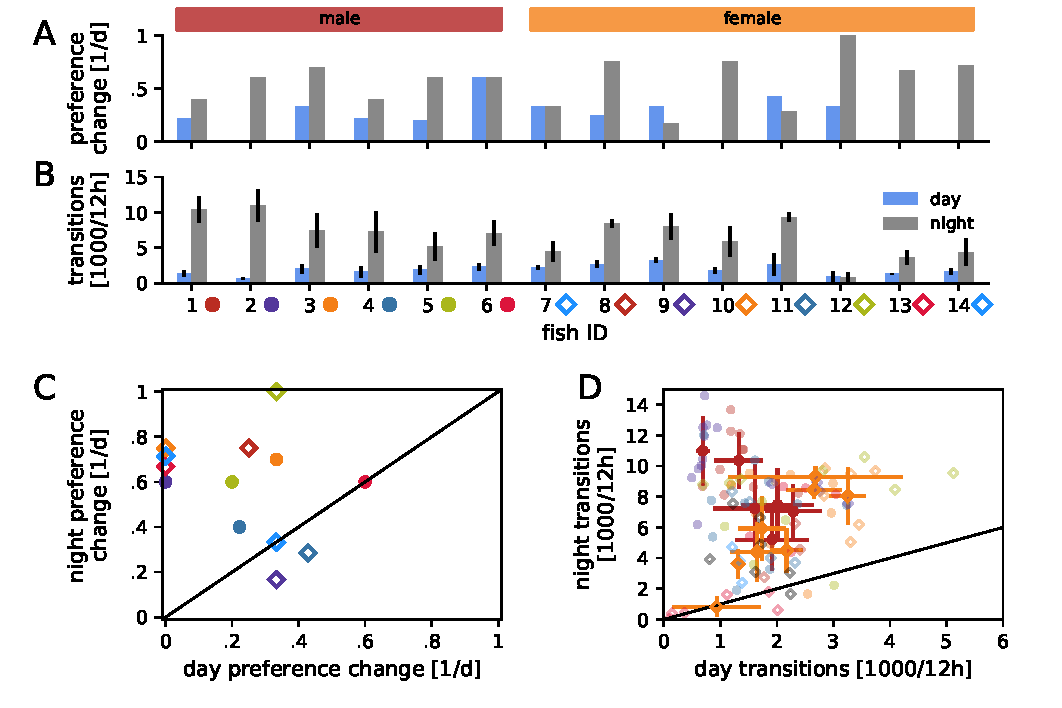
\includegraphics[width=1\linewidth]{transitions}}}
  \caption{\label{transitions} Transitions of habitat preference and
    between habitats. \figitem{A} Probability of changing the
    preferred habitat from one day (blue) or night (grey) to the next
    for each fish. \figitem{B} Transition rates, i.e., number of
    detected transitions between habitats per 12\,h, averaged over
    days (blue) or nights (grey) with standard deviation.
    \figitem{C} Probabilities of changing preference of night habitats
    vs. preference changes of day habitats from
    \panel{A}. \figitem{D} Transition rates during the day
    vs. transition rates at night from \panel{B}.  Transition
    counts averaged over days and nights with standard deviation are
    shown for each male (red) and female (orange). Symbols in
    \panel{C}~\&~\panel{D} indicate fish ID as in \panel{B}.}
\end{figure*}

\subsection{Transitions between habitats}
Fish frequently moved between habitats (\subfigrefb{transitions}{B}). The EOD frequency of males correlated negatively with the number of transitions between habitats during the day and positively during the night (Spearman's rank correlation: $r=-0.47$, $p<0.01$ and $r=0.55$, $p<0.001$, respectively). That is, high-frequency males were more territorial during the day and more explorative at night than low-frequency males. In females, transition counts correlated positively with EOD frequency during both day and night (Spearman's rank correlation: $r=0.55$, $p<0.001$ and $r=0.45$, $p<0.01$). Therefore, females with higher EOD frequency were more active.

Both males and females switched habitats significantly more often during the night than during the day (\subfigrefb{transitions}{D}). The more stationary males were during the day, the more explorative they were at night (Spearman's rank correlation: $r=-0.49$, $p<0.001$). On the other hand, female transition counts during day and night were positively correlated ($r=0.53$, $p<0.001$). No such correlations existed for individual fish.

Transition times, i.e., the time intervals between habitat transitions, were approximately exponentially distributed (\eqnref{expdist}, \subfigrefb{transitiontimes}{A}). Such exponential distributions are generated by Poisson point processes where the probability of
an event (here a transition to another habitat) is the same for each time point and independent of previous events, like for example radioactive decay or state transitions of ion channels. There was no distinguished time scale that separated activity phases from resting phases. Transition rates (\subfigsref{transitions}{B}, \subfref{transitiontimes}{B}) were generally quite high and average to 0.1\,Hz. They were significantly larger during the night than during the day for both, males (Mann-Whitney U: $U=0$, $p<0.01$, $d =
4.05$) and females (Mann-Whitney U: $U=8$, $p<0.05$, $d = 1.58$), and were independent of sex (\subfigrefb{transitiontimes}{B}).

Averaged weighted transition times, \eqnref{weightedtime}, better capture differences on long time scales, reflecting non-moving fish. On average weighted transition times were 20\,min during the day and 3\,min at night (\subfigrefb{transitiontimes}{C}, Mann-Whitney U: males $U=0$, $p<0.01$, $d=1.41$, females $U=8$, $p<0.05$, $d=0.34$).

Transitions of individual fish were independent from other fish entering the habitat (not shown). The distribution of times between a fish entering a habitat and another fish leaving
the same habitat showed statistically significant (Kolmogorov-Smirnov test, $p<0.001$) but small differences to a distribution generated for times of a fish entering a randomly chosen habitat drawn from a uniform distribution (Cohen's $d$: $0.02<d<0.08$).

\begin{figure*}[t]
  \showfigure{\centerline{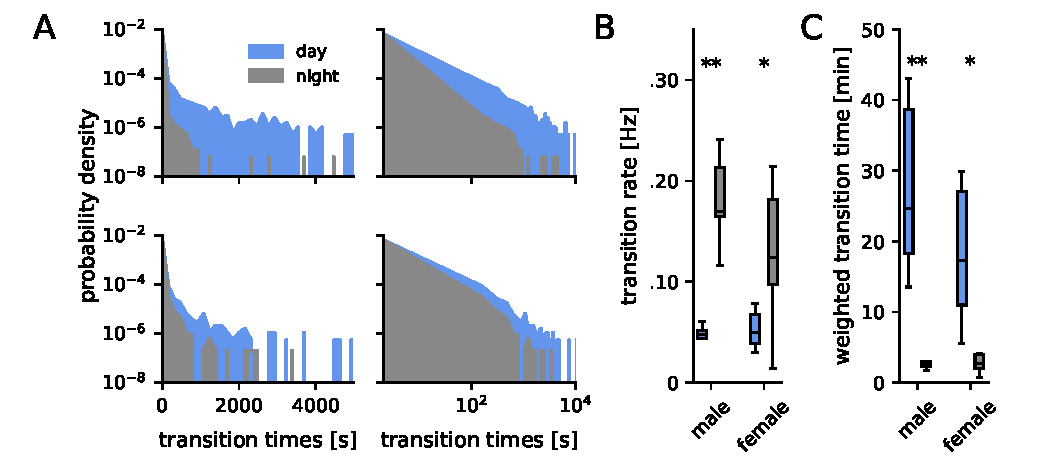
\includegraphics[width=1\linewidth]{transition_times}}}
  \caption{\label{transitiontimes} Transition times. \figitem{A}
    Probability density of transition times (time span spent
    consecutively within one habitat) during the day (blue) and the
    night (grey) for one example male (top, fish ID 4) and female
    (bottom, fish ID 10). \figitem{B} Corresponding transition rates
    obtained from fitting an exponential to the distributions of
    transition times. \figitem{C} Averaged weighted transition times
    \eqnref{weightedtime}. Asterisks indicate significant differences:
    ** $p<0.01$, and * $p<0.05$.}
\end{figure*}

\subsection{Sensitivity analysis}
Since we based the sex of the fish on EOD frequency only, we repeated all analysis for different EOD frequency thresholds separating males from females. For up to two males reassigned to females and vice versa the sex dependent results in the contexts of \subfigsref{transitions}{C, D}, \subfref{transitiontimes}{B, C} did not change. All significant levels as well as effect sizes stayed in the same range.

\section{Discussion}
We observed movement patterns and habitat preferences in a population of fourteen brown ghost knifefish, \lepto{}, in a large indoor tank over 10 days. During the day, these
nocturnal fish distributed themselves quite uniformly in habitats providing appropriate retreat sites between stones or plants. Activity at night was characterized by strong explorative movements where fish frequently changed between habitats and the open water. In male fish, high EOD frequency correlated with more territorial behavior during days and a more explorative personality at night, whereas in female fish EOD frequency was positively correlated with movement activity during both day and night.

\subsection{Nocturnal activity}
Despite the well supported common notion of weakly electric fish being nocturnally active \citep{Lissmann1965, Zupanc2001, Henninger2018}, our data show that phases of activity, as indicated by short transition times between the habitats, occurred in similar ways both at night and during the day (\subfigref{transitiontimes}{A}). There was no qualitative difference between day and night. During the day, phases of inactivity were prolonged
about ten-fold in comparison to the ones at night (\subfigref{transitiontimes}{B,\,C}).
Otherwise, activity, as quantified by transitions between habitats, occurred randomly and independently of each other. This fits well with the description of stochastic onsets of activity phases in \textit{Gymnotus} \citep{Jun2014}.

\subsection{Retreat site selection}
Selection of an appropriate retreat site has profound effects on the animal's physiological condition and fitness \citep{Rosenzweig1981, Huey1991}. All of the preferred retreat sites in our experiment offered appropriate places where fish could hide. This fits well to field observations where fish were also found hiding under submerged logs, between roots, or in leaf litter during the day \citep{Hopkins1974, Hagedorn1988, Westby1988}. Our data
demonstrates that, at least in captivity, most fish do not depend on specific retreat sites, like for example stacked stones, but rather change between many available types of microhabitats.

In small tanks in the laboratory males often compete over tubes provided for refuge \citep{Hopkins1974, Hagedorn1988, Fugere2011}. In the presence of enough tubes, male
\lepto{} preferred to occupy tubes alone, but females were sometimes found together in single tubes \citep{Dunlap2002}. Fish had clear preferences when presented with a variety of tubes of different dimensions and opacity \citep{Dunlap2002}.

In our study fish showed individual preferences for different habitats (\subfigref{habitatpref}{A}). The grass and gravel habitat accommodated the most individuals simultaneously, and the open water the least (\subfigref{habitatpref}{C}). This indicates either differences in general habitat quality or differences in the actual number of available suitable retreat sites in each of the habitats. The fraction of males found in each habitat on average did not deviate from the expectation given the total number of males and females (\subfigref{habitatpref}{D}). Thus, group composition on the scale of a whole
habitat was not influenced by the hierarchical status of individual fish. However, our experimental design did not allow to resolve group compositions on a finer spatial scale of specific retreat sites within each habitat. Our data therefore do not contradict an influence of hierarchical status on retreat site selection as reported by \citet{Dunlap2002}.

\subsection{Social dominance}
The EOD and its modulations convey information about species, sex, status and intent of individuals (e.g., \citealp{Hagedorn1985, Stamper2010, Fugere2011}). In \lepto{} EOD frequency correlates with body size \citep{Dunlap2002b, Triefenbach2003}. Furthermore, dominant males in breeding contexts in the laboratory \citep{Hagedorn1985} as well as in the field \citep{Henninger2018}, and in tube selection contexts \citep{Dunlap2002, Fugere2011} had higher EOD frequencies. We here reported a more subtle variant of dominance. Male fish
with higher EOD frequency moved less between habitats during the day and showed increased movement activity at night compared to males with lower EOD frequency. These increased
nocturnal movement activities could reflect frequent fights for dominance \citep{Tallarovic2005}, as the approaching EOD frequencies of the fish suggest (\subfigrefb{eodtraces}{C}). Contrary to the expectation of fish fighting for dominance, the time points of fish leaving a habitat were independent from fish entering the respective habitat. A closer inspection of the EOD frequency traces for communication signals like rises and chirps \citep{Zakon2002} could help classify different types of movement activities and interactions in the future \citep{Triefenbach2008}. In females, EOD frequency did not appear to be correlated with dominance \citep{Dunlap2002}. However, we found that EOD frequencies of females were positively correlated with movement activity during both day
and night. Rather than an indication of hierarchical status, EOD frequency seems to indicate individual activity personalities \citep{Sih2004}.

\subsection{Conclusion}
Many laboratory studies on the behavior of weakly electric fish focused on specific questions that were tested in temporally and spatially limited experimental settings \citep{Hopkins1974,Hagedorn1985,Nelson1999,Tallarovic2002,Hupe2008,Triefenbach2008}. Recent advances in recording techniques \citep{Madhav2018,Henninger2018} allowed us to continuously monitor a population of weakly electric fish in a large tank with a more natural-like setting for many days. In particular, we did not force the fish into specific behaviors,
but rather, extracted behavioral activity patterns from the data \citep{Gomez2014}. In this way, we revealed personality like differences in territoriality and explorative movements
\citep{Sih2004}. In both males and females these were correlated with EOD frequency, suggesting EOD frequency as an indicator for more explorative personalities in both sexes, and territoriality in males.

%\bibliographystyle{jneurosci}
%\bibliography{../journalsabbrv,../references}


\cleardoublepage
\graphicspath{{chapter_4_competition/figures/}}

\chapter[Staged competition and opponent assessment]{Staged competition and opponent\\ assessment}
\label{Competitions}

\textbf{The literal content of this chapter has already been published as:}\\  
Till Raab, Sercan Bayezit, Saskia Erdle, Jan Benda (2021) Electrocommunication signals indicate motivation to compete during dyadic interactions of an electric fish. \textit{Journal of Experimental Biology} 224(19):Jeb242905.

\paragraph*{Contributions}
For this scientific project Till Raab designed the experiments, collected and analyzed the data, performed post-processing of electric EOD recordings, generated the displayed figures, and wrote the manuscript. 
Saskia Erdle and Sercan Bayezit collected the data while being supervised by Till Raab. Sercan Bayezit additionally  detected agonistic event in the complementary IR-video recordings and provided sketches of agonistic interactions between fish displayed in \subfigref{trial}{C, D}. 
Jan Benda discussed the experiments, advised data analysis, and assisted writing the manuscript. 

\begin{quote}
\begin{center}
\large\textbf{Abstract}
\end{center}
Animals across species compete for limited resources. Whereas in some species competition behavior is solely based on the individual's own abilities, other species assess their opponents to facilitate these interactions. Using cues and communication signals, contestants gather information about their opponent, adjust their behavior accordingly, and can thereby avoid high costs of escalating fights. We tracked electrocommunication signals known as ``rises'' and agonistic behaviors of the gymnotiform electric fish \Lepto{} in staged competition experiments. A larger body size relative to the opponent was the sole significant predictor for winners. Sex and the frequency of the continuously emitted electric field only mildly influenced competition outcome. In males, correlations of body size and winning were stronger than in females and, especially when losing against females, communication and agonistic interactions were enhanced, suggesting that males are more motivated to compete. Fish that lost competitions emitted the majority of rises, but their quantity depended on the competitors' relative size and sex. The emission of a rise could be costly since it provoked ritualized biting or chase behaviors by the other fish. Despite winners being accurately predictable based on the number of rises after the initial 25\,min, losers continued to emit rises. The number of rises emitted by losers and the duration of chase behaviors depended in similar ways on physical attributes of contestants. Detailed evaluation of these correlations suggests that \lepto{} adjusts its competition behavior according to mutual assessment, where rises could signal a loser's motivation to continue assessment through ritualized fighting.
\end{quote}
\hfill

\section{Introduction}  % 930 words

Across animal species, fighting is a key behavior to secure access to limited resources \citep{Cluttonbrock1979, Chapman1995, Markham2015}. However, competition is costly because of the energy and time allocated to it, and the increased risk of injury or death (e.g. \citealp{Briffa2004}). Therefore, individual behavioral decisions during contests are strongly dependent on the associated potential benefits and costs \citep{ArnottElwood2008, ArnottElwood2009}. Often, the best predictor for the outcome of competitions is the contestants’ fighting ability, also called resource holding potential (RHP; \citealp{Parker1974}). Usually, larger and stronger individuals win contests, because their physical advantages (higher RHP) directly reflect their increased endurance and potential to inflict damage \citep{Archer1988}. Additional factors such as weaponry, experience and sex, or positional advantages also influence RHP (reviewed in \citealp{ArnottElwood2008}).

Behaviors and the course of competition have been shown to be either based on the assessment of solely the individual’s own RHP or by integrating both the individual and opponent’s RHP \citep{Taylor2001, Enquist1990, Huyghe2005}. In the first case (self-assessment), costs resulting from competition are accumulated until an endurance threshold, set by an individual’s RHP, is reached and the respective individual retreats \citep{ArnottElwood2009}. Competition costs either arise exclusively from an individual’s own behaviors (pure self-assessment, \citealp{Taylor2003}) or are supplemented by costs inflicted by opponents (cumulative assessment, \citealp{Payne1998}). In both cases, no direct information about an opponent and its RHP is gathered. Alternatively, in ``mutual assessment'', the contestants assess each other’s RHP, compare it to their own, and adjust their behavior according to the difference \citep{EnquistLeimar1987}. The huge benefit of this strategy is its economic efficiency. Individuals can recognize their inferiority and retreat long before their endurance threshold is reached, thereby saving metabolic costs for both competitors.

Besides passive cues signaling RHP, actively produced communication signals may facilitate interactions during animal conflict \citep{ArnottElwood2009, Seyfarth2010}. They can directly indicate and reflect an individual’s RHP \citep{Davies1978, Cluttonbrock1979}, but also convey additional information influencing contest and its outcome, like motivation and behavioral intent (e.g. aggression: \citealp{Kareklas2019, Westby1970}; or submission: \citealp{Hupe2008, Silva2012}) or social status \citep{Fernald2014}. Such low-cost signals have been shown to reduce the intensity and duration of contests or even convey sufficient information to resolve conflicts without the necessity of physical competitions \citep{Parker1974, Cluttonbrock1979, Jason1990}.

To prevent high costs of repetitive fights with the same opponents, dominance hierarchies are established in various species \citep{Creel1996, Janson1985, Cluttonbrock1979}. In dominance hierarchies the necessity of fighting is reduced since access to resources is regulated through social status, favoring those individuals of higher rank \citep{Wauters1992, Taves2009}. The organization and characteristics of dominance hierarchies vary across species \citep{Janson1985, Cigliano1993, Sapolsky2005}. While in group-living species complex social structures, such as a leader-follower dynamic, can emerge \citep{Strandburg2018}, in solitary species, dominance is rather associated with resource-based benefits, such as the occupation of higher quality territories and increased reproductive success (e.g. \citealp{Cigliano1993}). Differences in the abundance and dispersion of food can further lead to variations regarding the skewness in access to resources across social ranks. In bottom-up egalitarian hierarchies, resources are more equally distributed \citep{Sapolsky2005}, whereas in top-down despotic hierarchies, access to resources is strongly skewed in favor for dominant individuals \citep{Kappeler2008}.

Dominance hierarchies have also been suggested for the nocturnal gymnotiform electric fish \Lepto{} \citep{Dunlap2002, Stamper2010, Raab2019}. \lepto{} competes for mates only during the mating season \citep{Hagedorn1985, Henninger2018}, at other times they compete for optimal shelters \citep{Dunlap2002}. The corresponding competitions are characterized by ritualized fighting behaviors accompanied by electrocommunication signals \citep{Triefenbach2008, Smith2013}. While body size has been shown to be the main determinant for the outcome of competitions in gymnotiformes \citep{Silva2012, Triefenbach2008, Dunlap2002}, the influence of other factors such as sex and communication signals, require further investigation.

Electric signaling has been shown to be an integral aspect of agonistic behaviors in gymnotiform fish \citep{Westby1970, Silva2012, Hupe2008, Henninger2018}. The frequency of their continuous electric organ discharge (EOD) has been suggested to signal an individual's physical condition, dominance status or aggressiveness \citep{Westby1970, Hagedorn1985, Cuddy2012}. The sexually dimorphic EOD frequency (EODf) of \lepto{} indicates identity and sex \citep{Henninger2020}, with males having higher EODfs than females \citep{Meyer1987}. While some studies also suggest that higher EODf indicates dominance \citep{Hagedorn1985, Dunlap2002, Henninger2018, Raab2019}, others were not able to replicate this correlation \citep{Triefenbach2008}.

For generating distinct electrocommunication signals, electric fish modulate their EODf on various time scales \citep{Benda2020}. So-called ``chirps'' are several types of brief (10 -- 500\,ms), transient increases in EODf \citep{Engler2000, Zakon2002,Hupe2008b}. ``Small'' and ``long'' chirps are used in courtship for synchronizing spawning \citep{Henninger2018} and at the same time the very same small chirps are used as submissive signals to reduce attacks in agonistic encounters \citep{Hupe2008, Henninger2018}. Another category of electrocommunication signals, so-called ``rises'', are characterized by a moderate increase in EODf by no more than a few tens of Hertz followed by an approximately exponential decay back to baseline EODf from within a second up to almost a minute \citep{Hopkins1974, Engler2000, Tallarovic2002, Zakon2002}. The function of rises is still controversial. They have been suggested to signal aggression or motivation to attack \citep{Tallarovic2005, Triefenbach2008}, submission \citep{Hopkins1974, Serrano2003}, ``victory cries'' \citep{Dye1987}, to evoke or precede attacks \citep{Hopkins1974, Triefenbach2008}, or to simply be a general expression of stress \citep{Smith2013}. An enhancement of sensory acquisition by rises is highly unlikely, because the small increase in EODf only marginally influences encoding in electroreceptor afferents \citep{Walz2014}.

Using recently developed techniques for tracking electrocommunication signals in freely behaving electric fish \citep{Henninger2018, Madhav2018, Henninger2020} in addition to infrared video recordings, we recorded electric and physical interactions of pairs of \lepto{} in staged competitions over a superior shelter. Compared with previous studies we significantly expanded the observation times (from 10\,min to 6\,h) and the number of interacting pairs of fish. We evaluated the influence of body size, weight, sex and EODf on the outcome of competitions. By analyzing the relationships between rises, agonistic interactions and physical difference between competitors we were able to uncover the fish’s assessment strategy, quantify behavioral difference between the sexes, and identify the potential uses of rises of \lepto{} during competitions.

\section{Methods}    % 1480 words
\subsection{Animals}

A total of 21 mature \Lepto{} (9 males, 12 females) not in breeding condition, obtained from a tropical fish supplier, were used. Fish were selected randomly from multiple populations to reduce familiarity effects and sorted into four mixed-sex groups of five or six fish (males/females: group 1: 2/4; group 2: 1/4; group 3: 3/2; group 4: 3/2). Males were identified by their higher EODf (see below) and elongated snout. The sex of one-third of the fish was verified after the competition experiments via post-mortem gonadal inspection in the context of electrophysiological experiments (approved by Regierungspr\"asidium T\"ubingen, permit no. ZP 1/16) which verified sex assignments for most of the fish with EOD frequencies close to the male-female cut-off of 740 Hz (\Subfigrefb{fishsetup}{A}). Fish were housed individually in 54 liter tanks with a 12\,h:12\,h light:dark cycle prior to the experiments and in between competition trials. Each tank was equipped with a plastic tube for shelter, a water filter and an electrical heater. Water temperature was constant at $25\pm0.5$\,\celsius{} and water conductivity was 200\,\micro\siemens\per\centi\meter. Fish were fed frozen \textit{Chironomus plumosus} daily. The competition experiments complied with national and European law and were approved by the Regierungspr\"asidium T\"ubingen (permit no. ZP 04/20 G)

\subsection{Setup}

The competition experiments were run in a 100\,liter tank equipped with a 10\,cm long and 4\,cm wide PVC half-tube as a superior shelter in the center, surrounded by four additional, less optimal shelters (two 5\,cm long, 4\,cm diameter PVC half-tubes and two $3\times 5$\,\centi\meter\squared{} tables, \Subfigrefb{fishsetup}{C}). Water temperature and conductivity as well as light:dark cycle were identical to those in the housing tanks. A heating mat was placed below the tank and powered with DC current. Two air-powered water filters were placed behind PVC boards with netted windows in the corners of the tank to avoid offering additional shelter. 15 monopolar electrodes at low-noise buffer headstages were mounted on the bottom of the tank. The reference electrode was placed behind a PVC board in one corner of the tank. Electric signals were amplified ($100\times$ gain, 100\,Hz low-pass filter, EXT-16B, Npi electronic, Tamm, Germany) digitized at 20\,kHz per channel with 16 bit resolution (USB-1608GX-2AO, Measurement Computing) and stored on 64\,GB USB sticks using custom written software running on a Raspberry Pi 3B. Water temperature was measured every 5\,min (Dallas DS18B20 1-wire temperature sensor). Infrared videos were recorded at 25 frames s$^{–1}$ with a camera (Allied Vision Guppy PRO) mounted on top of the
tank for all trials of groups 3 and 4. The tank was continuously illuminated by $2\times 4$ infrared lights (ABUS 840\,nm) located on the long sides outside the tank. For the synchronization of video and electric recordings we used LED-light pulses of 100\,ms duration triggered by the computer-amplifier system in intervals of 5\,s. The LED was mounted on the edge of the tank not perceivable by the competing fish, but detectable in the video recordings. The tank, camera and lights were placed inside a Faraday cage.

\subsection{Experimental procedure}

In each competition trial two fish were freely swimming and interacting in the experimental tank for 6\,h. Participating fish were taken from their housing tanks and simultaneously released into the experimental tank. The first 3\,h of each trial took place during the dark phase and the second 3\,h during the light phase of the circadian rhythm the fish were accustomed to. This limited the experiment to one trial per day. The winner of each trial was identified by its presence within the superior shelter during the light-phase of the trial. Fish were transferred back into their housing tanks after the trial. Pairings for each trial were selected systematically to (i) ensure all possible combinations within each group to be tested (10 combinations for groups of five fish, 15 for the group with six fish), (ii) keep the experience level for all fish equal, and (iii) prevent a single fish from being tested on two consecutive days. Weight and length (body size) of each fish was assessed once a week starting in the week before the competition trials.

With 21 fish in four groups, we ended up with a total of 45 pairings and trials. Technical failure led to loss of the electric recordings for the initial four trials of group 4. In another three trials, we were unable to extract EODf traces and electrocommunication signals from the electric recordings because the EODf difference between fish were too low ($<0.5$\,Hz). In a single trial, which we discuss separately, we were unable to determine the winner, because both fish shared the superior shelter at the end of the trail. The remaining 37 trials were analyzed in detail.

\subsection{Preprocessing of electric and video recordings}

After computing spectrograms for each channel with fast Fourier transformation (FFT, $n_{\rm fft}=2^{15}$, corresponds to 1.63\,s, 80\,\% overlap) we first detected peaks in a power spectrum summed over the channels and assigned them to the fundamental EODfs and their harmonics of the two fish. Based on EODfs and the distribution of power in the channels, we tracked electric signals over time and obtained EODf traces for each of the two fish \citep{Henninger2018,Henninger2020, Madhav2018}.

To assess baseline EODf, we computed the 5th percentile of non-overlapping, 5\,min long EODf trace snippets. EODf is sensitive to temperature changes, which were inevitable throughout the single trials and averaged at 1\,\celsius. We computed the $Q_{10}$ values resulting from temperature and EODf differences of each 5\,min snippet and used the median of 1.37 over all fish to adjust each fish’s EODf to 25\,\celsius{} (EODf$_{25}$). The EODf$_{25}$ was used to assess an individual’s sex, with EODf$_{25} > 740$\,Hz assumed to originate from males. As noted above, the sex of half of the fish was verified via post-mortem gonadal inspection.

EODf difference for each pair of fish was estimated from the difference of the median baseline EODfs of the competitors during the light-phase of each trial, where EODfs stayed comparably stable. Rises were identified by detecting their characteristic onset peak in
each EODf trace, based on a minimum difference of 5\,Hz between a peak and the preceding trough \citep{Todd1999}. Then, the size of the rise, its maximum increase in EODf, was calculated by subtracting the baseline EODf from this peak frequency.

We manually extracted two categories of agonistic interactions from the infrared video recordings using the event logging software BORIS \citep{Friard2016}. For agonistic interactions without physical contact that were characterized as high velocity, directed movements towards a competitor (e.g. chase behavior), we recorded onset and end times. Agonistic physical contacts between competitors such as ritualized biting or head bumping were detected as point events.

\subsection{Data analysis}

The recorded data and custom analysis scripts are available on request. Data were analyzed in Python version 3.6.8 using numpy \citep{vanderWalt2011}, scipy \citep{Oliphant2007} and matplotlib \citep{Hunter2007} packages. All averages are given with their standard deviation. Mann-Whitney U-tests were used to assess significance of differences between two populations and Pearson's test and correlation coefficient r for assessing correlations. The influence of various factors on competition outcome was quantified by paired t-tests and by the area under the curve (AUC) of a receiver-operating characteristics (ROC). Generalized linear models (GLM):
\begin{equation}
 \label{glmmodel}
 y = \frac{1}{1 + \exp{(c_0 + \sum c_i \cdot x_i)}},
\end{equation}
with a logistic link function were used to estimate the combined effects of several factors $x_i$ (continuous: EODf, size, $\Delta$EODf and $\Delta$size, categorical: sex), linearly combined with coefficients $c_i$ and an offset $c_0$, on the outcome of the competitions $y$ (winner or loser). The performance of the GLMs was again assessed by the AUC of a ROC analysis. Standard deviations of AUC values were obtained by 1000 times bootstrapping the data.

To evaluate the influence of the contestants' physical attributes on the quantity of emitted rises throughout a trial, simple correlations were supplemented by multiple linear regression models. For each model we performed backwards elimination model selection with an elimination criterion of $\alpha > 0.05$.

Temporal coupling between rises and agonistic interactions was quantified by a cross-correlation analysis, i.e. by estimating the average rate of rises centered on agonistic events (onset of chase behaviors or physical contact). For this the temporal differences, $\Delta$t, between agonistic onsets and rises up to $\pm 60$\,sec were convolved with a Gaussian kernel with a standard deviation of 1\,s. Statistical significance was assessed by a permutation test. The null hypothesis of rises not being correlated with agonistic interaction events was obtained by computing the cross-correlation as described above from 1000 random variants of shuffled rise intervals. From this distribution we determined the 1st and 99th percentiles. In addition, we computed the 98\,\% confidence interval for the estimated cross-correlation by 1000 times jack-knife resampling where we randomly excluded 10\,\% of the rises.

We used a time window 5\,s prior to agonistic onsets to quantify the average number of rises per agonistic event and to compare them with the corresponding time fractions, the number of agonistic events multiplied with the 5\,s window relative to the total dark period time of 3\,h. The time window of 5\,s was chosen to approximately cover the time of significantly elevated rise rates that we observed before the agonistic events in the cross-correlation
analysis.

\section{Results}   % 3600 words
In 37 trials we observed and analyzed pairs of \lepto{} (6 male pairs, 10 female pairs and 21 mixed-sex pairs) competing for a superior shelter. The 9 males differed from the 12 females by their higher EOD frequency as expected from the sexual dimorphism in EODf in \lepto{}. Fish size ranged from 9 to 19 cm and was independent of sex ($U=51.5$, $p=0.44$, \Subfigrefb{fishsetup}{A}). Fish size strongly correlated with body weight (3.3--20.3\,g, $r=0.94$, $p<0.001$, \Subfigrefb{fishsetup}{B}) and we therefore excluded weight from the following analysis.

\begin{figure}[ht!]
  \centerline{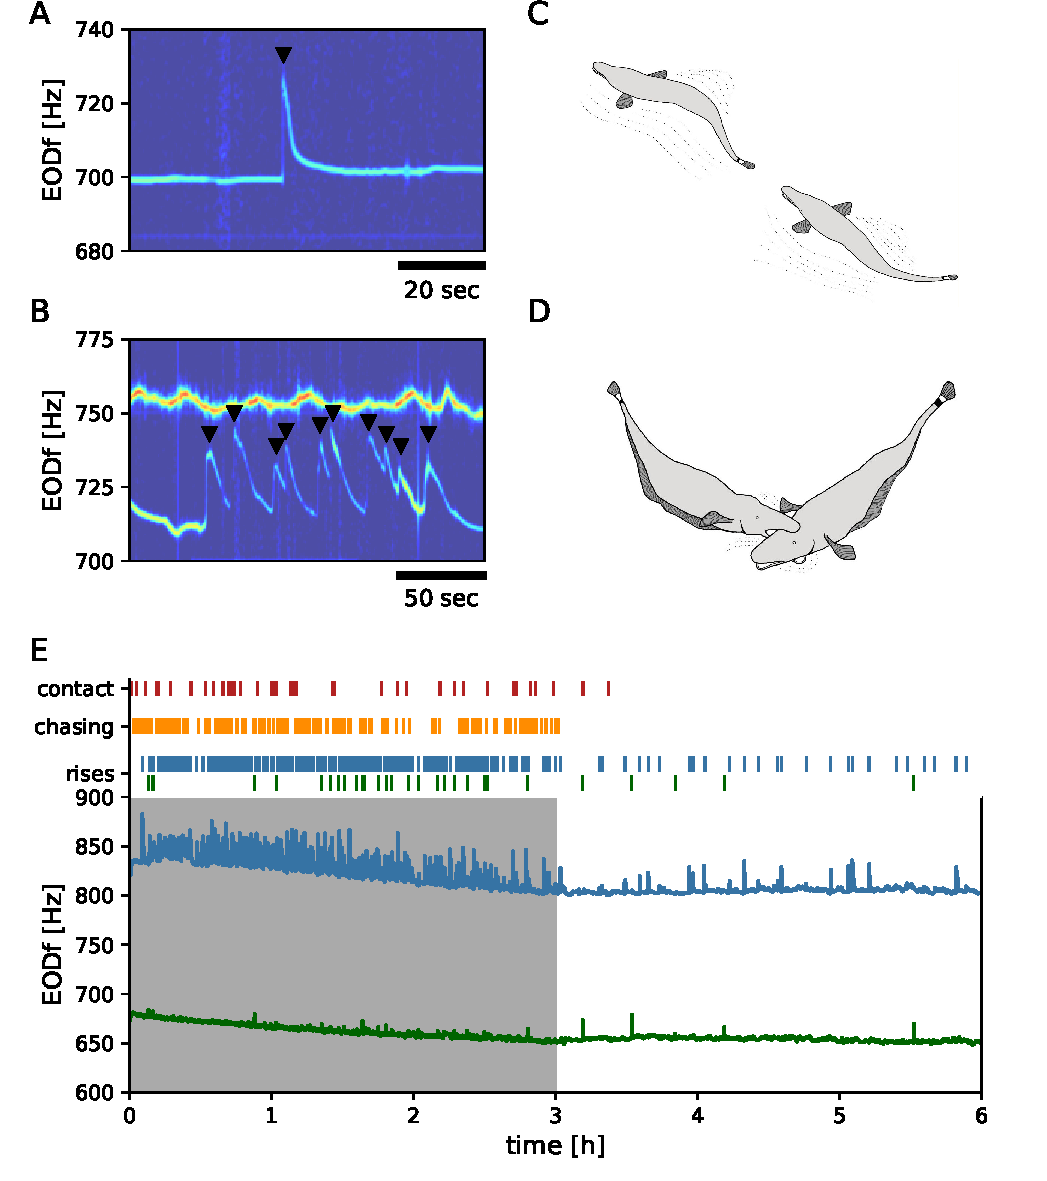
\includegraphics[scale=0.75]{Fig1CompetitionExample}}
  \caption{\label{trial} Behaviors and interactions of \Lepto{} during a typical competition trial. \figitem{A} Spectrogram of an electric recording comprising the EODf trace of a fish while emitting a rise as communication signal. Rises are abrupt increases in EODf followed by an exponential decay back to baseline EODf. Rises were detected using their characteristic onset peak (black triangle). \figitem{B} Spectrogram of a 200\,s section of an electric recording comprising EODf traces of two fish. In the lower EODf trace a series of 10 rises can be seen. \figitem{C, D} Ritualized agonistic interactions in A. leptorhynchus comprise non-physical chasing (panel~\panel{C}) and short physical agonistic interactions such as biting or head bumping (panel~\panel{D}). Both were initiated by fish later winning a trial. \figitem{E} A. leptorhynchus continuously emits EODs with an individual specific frequency. EODf traces of both competing fish (blue male and green female, bottom panel), time points of physical contacts, onsets of chase behavior, and detected rises (top panels) recorded during the full 6\,h trial with the first 3\,h in darkness (gray) and the last 3\,h during light.}
\end{figure}

We were able to track electric behaviors of the competitors based on the individual-specific EODf traces, including the detection of rises (electrocommunication signals, \Subfigrefb{trial}{A,B}). Complementary infrared video recordings obtained during the 20 trials of group 3 and 4 were used to detect ritualized agonistic behaviors, i.e. chasing (\Subfigrefb{trial}{C}) and physical contacts such as biting or head bumping (\Subfigrefb{trial}{D}). In a typical competition trial (\Subfigrefb{trial}{E}), the competing fish's overall activity was much higher during the initial, 3\,h dark phase as demonstrated by the higher rates of agonistic interactions and rise emission. During the subsequent 3\,h light phase, the activity ceased almost entirely and one fish spent substantially more time within or closer to the superior shelter ($99.27 \pm 0.006$\,\%). This fish was identified as the winner. EODfs of the two fish usually differed clearly and decreased over the course of the experiment because of slightly decreasing water temperature.

\subsection{Larger fish win competition}

\begin{figure}[t]
  \begin{minipage}[t]{0.5\textwidth}\mbox{}\\[-2ex]  
    \centerline{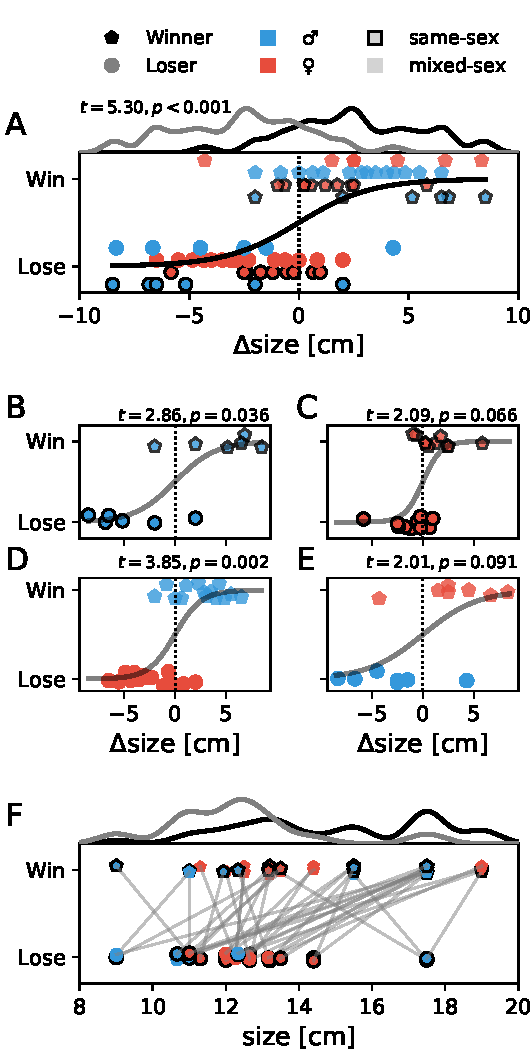
\includegraphics[scale=0.75]{Fig2bodysize}}
  \end{minipage}
  \hfill
  \begin{minipage}[t]{0.45\textwidth}
  \caption{\label{bodysize} 
  Body size and size difference of winners and losers. \figitem{A} Winners are larger than their opponents as indicated by a logistic fit and corresponding kernel histograms. \figitem{B--E} Winners are larger in all sex pairings and this effect was more distinct for winning males (\panel{B}, \panel{D}). \figitem{F} Distributions of absolute body size of winners and losers largely overlap. Gray lines connect pairs competing in a trial. Colors and marker style indicate different pairings and the outcome of competitions. Each competition trial contributes two data points, one for the winner and one for the loser. Blue represents males, red females. Pentagons indicate winners, circles losers. Black marker edges indicate same-sex pairings. Winners and losers of each sex pairing are offset in panel A and jittered in panels~\panel{B}--\panel{F}.}
  \end{minipage}
\end{figure}

%\begin{wrapfigure}{r}{0.5\textwidth}
%  \vspace{-2ex}
%  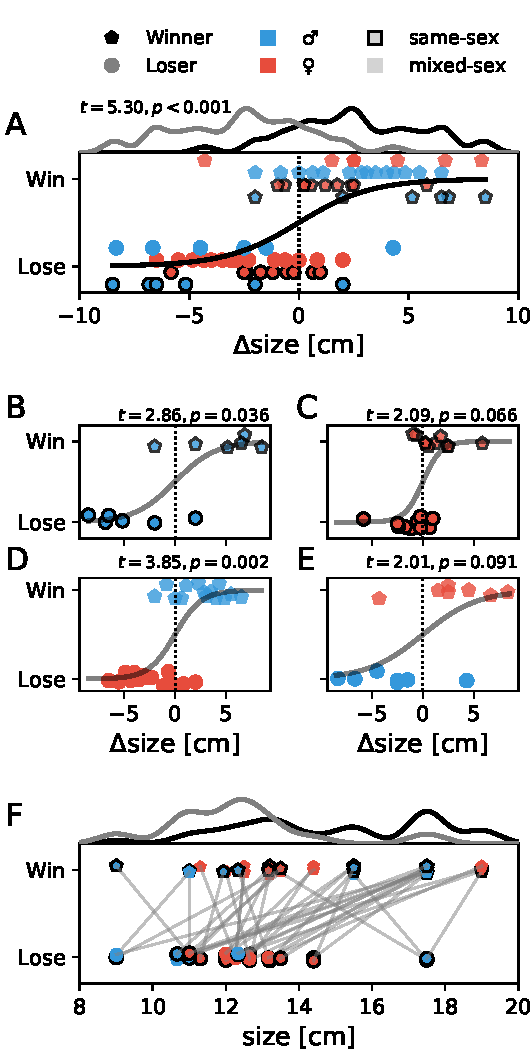
\includegraphics[width=1\linewidth]{Fig2bodysize}
%  \caption{\label{bodysize} Body size and size difference of winners and losers. \figitem{A} Winners are larger than their opponents as indicated by a logistic fit and corresponding kernel histograms. \figitem{B--E} Winners are larger in all sex pairings and this effect was more distinct for winning males (\panel{B}, \panel{D}). \figitem{F} Distributions of absolute body size of winners and losers largely overlap. Gray lines connect pairs competing in a trial. Colors and marker style indicate different pairings and the outcome of competitions. Each competition trial contributes two data points, one for the winner and one for the loser. Blue represents males, red females. Pentagons indicate winners, circles losers. Black marker edges indicate same-sex pairings. Winners and losers of each sex pairing are offset in panel A and jittered in panels~\panel{B}--\panel{F}.}
%\end{wrapfigure}

The larger fish of each pairing was more likely to win the competition ($t=5.3$, $p<0.001$, \Subfigrefb{bodysize}{A}). Winners are correctly assigned with a probability of 90\,\% based on size difference (in the sense of the AUC of a ROC analysis, \Subfigrefb{glm}{C}) In particular, in trials won by males, most of the winners were larger than the losers (male--male: 5 out of 6, $t=2.9$, $p=0.036$; male--female: 11 out of 14, $t=3.9$, $p=0.002$; \Subfigrefb{bodysize}{B, D}). In trials won by females, this influence of size difference was similarly pronounced but not significant (female--female: 8 out of 10 winners were larger, $t=2.1$, $p=0.07$; female--male: 6 out of 7 winners were larger, $t=2.0$, $p=0.09$; \Subfigrefb{bodysize}{C, E}). In 12 of the 21 mixed-sex pairings the males were larger than the competing females, of which only a single male lost. Of the nine larger females three lost. Absolute size, in contrast, did not predict competition outcome ($\text{AUC}=67$\,\%, \Subfigrefb{bodysize}{F}). Note that EODf did not correlate with size in either males or females (males: $r=0.47$, $p=0.20$; females: $r=0.04$, $p=0.90$) and that size was independent of sex (\Subfigrefb{fishsetup}{A}).

\subsection{Fish with higher EODf seem to win competitions}

Previous studies suggest EODf to be an indicator for dominance in \lepto{} \citep{Dunlap2002, Henninger2018, Raab2019}. Indeed, winning fish had on average higher EODfs in comparison to their opponents ($t=2.1$, $p=0.04$, \Subfigrefb{eodf}{A}). However, in same sex pairings analyzed separately, EODf did not predict competition outcome in either males ($t=0.79$, $p=0.47$, \Subfigrefb{eodf}{B}) or in females ($t=1.4$, $p=0.19$, \Subfigrefb{eodf}{C}), but the positive coefficient of the logistic regressions suggests a mild influence of EODf on the outcome of competitions. Furthermore, in mixed-sex pairings, winning males always had higher EODfs and winning females lower EODfs than their opponent, because of the sexual dimorphic EODfs in \lepto{} (\Subfigrefb{eodf}{D, E}). These mixed-sex competitions were more often won by males than by females (14 out of 21, Binomial test 14 or more males winning assuming equal chances for both sexes: $p=0.10$). This asymmetry results in an $\text{AUC}=82$\,\% for discriminating winners from losers based solely on sex as a rough proxy for EODf. Although the difference in EODf potentially contains more detailed information than sex alone, it does not discriminate winners from loser better than sex ($\text{AUC}=75$\,\%). Absolute EODf is even less informative about competition outcome ($\text{AUC}=65$\,\%, \Subfigrefb{eodf}{F}).

\subsection{Factors influencing competition outcome}

\begin{table}[t]
  \caption{\label{glm_table} Generalized linear model assessing the significance of
different physical factors on winning competitions. For each factor $i$ coefficients $c_i$ (Eqn.~\ref{glmmodel}), $t$-statistics, and significance is given. The competitors' size difference is the only significant factor of the model, indicating its predominant importance for winning competitions.}
  \renewcommand{\arraystretch}{0.9}
  \begin{center}
  \begin{tabular}{ L{2.5cm} R{2cm} R{2cm} R{2cm} }
    \hline
    Factor \trh & \trh Coefficient & \trh t-value & \trh p-value \\
    \hline
    Sex$_{f1}$ \trt & \trt $-1.437$ & \trt $-0.498$ & \trt $0.618$ \\
    Sex$_{f2}$ & $0.174$ & $0.067$ & $0.946$\\
    Size$_{f1}$ & $0.046$ & $0.255$ & $0.799$\\
    Size$_{f2}$ & $-0.371$ & $-1.918$ & $0.055$\\
    EODf$_{f1}$ & $0.002$ & $0.199$ & $0.842$\\
    EODf$_{f2}$ & $-0.005$ & $-0.456$ & $0.648$\\
    $\Delta$Size & $0.417$ & $2.392$ & $0.017$\\
    $\Delta$EODf & $0.007$ & $0.760$ & $0.447$\\
    \hline
  \end{tabular}
  \end{center}
  \renewcommand{\arraystretch}{1}
\end{table} 

We constructed a generalized linear model (GLM, Eqn.~\ref{glmmodel}), predicting the competition outcome based on all measured physical factors (size, size difference, EODf, EODf difference and sex; \Subfigrefb{glm}{A--C}). As expected from the single-factor analysis, size difference is the only factor significantly contributing to the prediction of winners ($t=2.4$, $p=0.017$, Table~\ref{glm_table}). The model correctly predicts the outcome of 34 of the 37 competition trials with an AUC of 94\,\% (\Subfigref{glm}{C}). Two-factor GLMs based on size differences and either sex or EODf differences perform similarly well ($\text{AUC} = 93$\,\%) and slightly better than size difference alone ($\text{AUC} = 90$\,\%), further questioning the role of EODfs in predicting competition outcome (\Subfigref{glm}{C}). The outcomes of competitions were independent of previous encounters. Auto correlations of win-lose histories did not differ from those of random sequences, where
winners and losers were assigned randomly (permutation test).

\subsection{Rises}

We detected in total 8530 rises using their characteristic onset EODf peak (\Subfigrefb{trial}{A, B}). The ``size'' of rises, the peak EODf relative to baseline EODf before, ranged from the detection threshold of 5\,Hz up to 68\,Hz with a mean of 17\,Hz. We were not able to detect any dependency of our results on the size of rises. In the following we therefore focus on an analysis of their quantity and timing.

\subsection{Losing fish emit more rises during the active-phase}

\begin{figure}[tp]
  \centerline{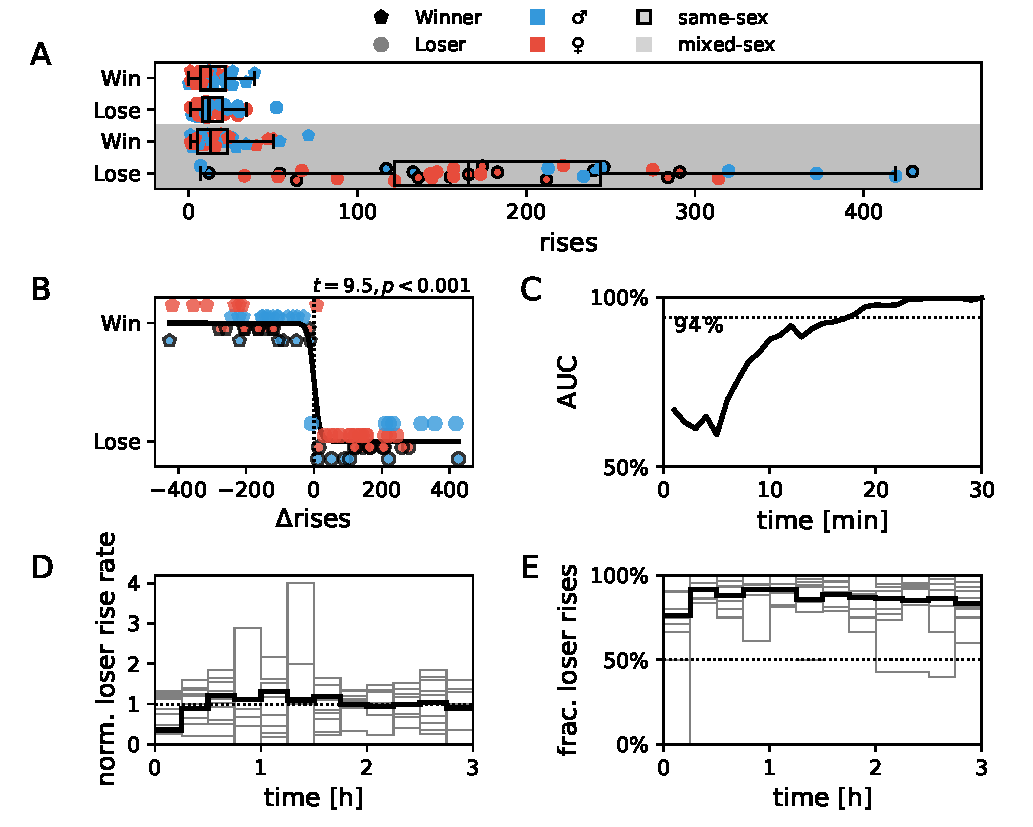
\includegraphics[scale=0.75]{Fig3Rises}}
  \caption{\label{EODfriserates} 
  Rise rates of winners and losers. \figitem{A} Rises are predominantly produced by losers of competitions during the dark phase (shaded). Winners during the dark phase produced equally few rises as both winners and losers during the light phase (white background). \figitem{B} Losers of competitions reliably produced more rises than winners in the dark, although absolute and relative numbers of rises varied considerably between trials. \figitem{C} Time-resolved discrimination performance between winners and losers based on differences in cumulative rise counts for the first 30\,min of the trials. The area under the curve (AUC) of receiver-operating characteristics (ROC) analysis asymptotes to almost 100\,\% after $\sim$25 min, indicating the outcome of the trials to be already determined the latest from this time on. For comparison, the dashed line at 94\,\% indicates the performance of the GLM including all physical characteristics of the fish from \Subfigrefb{glm}{C}. \figitem{D} Time course of loser rise rates during the dark phase. Rise rates of each trial (gray) were normalized to their mean rate. On average (black), rise rates reached a constant level after $\sim$30 min. \figitem{E} Fraction of rises of losing fish quantified in 15\,min time windows is consistently larger than 50\,\% (dashed line) throughout the whole dark period. Individual trials in gray, average over trials in black. Boxes indicate 25th and 75th percentiles with median; whiskers extend to the most extreme value within 1.5$\times$IQR outside the box.}
\end{figure}

Rises were primarily emitted during the dark phases, i.e. when fish were active ($t=6.7$, $p<0.001$). Fish that later in the light-phase did not occupy the superior shelter, produced 10-fold more rises in the dark phase ($184 \pm 105$) than their winning opponents ($18\pm 17$, $t=9.5$, $p<0.001$, \Subfigrefb{EODfriserates}{A}). Loser rise counts were highly variable. They ranged from 0 to 419 rises per trial with a coefficient of variation ($CV$) of $0.63$.

The difference between winners and losers in quantitative rise emission during the dark phase almost perfectly predicts winners ($\text{AUC} = 99.9$\,\%; \Subfigsrefb{EODfriserates}{B}). Initially, discrimination performance exponentially increases from chance level to maximum discrimination starting 5\,min after the beginning of a trial with a time constant of $\sim$5\,min (\Subfigrefb{EODfriserates}{C}). The prediction level of 94\,\% based on the physical factors (\Figrefb{glm}) is clearly surpassed after $\sim$20\,min. In that time losing fish emitted on average $7.0 \pm 5.7$ rises and winners just $1.2 \pm 1.2$.

The losing fish kept emitting higher numbers of rises than the winning fish throughout the dark phase of trials (\Subfigrefb{EODfriserates}{D}). In none of the trials did the competitors switch this behavior (\Subfigrefb{EODfriserates}{E}). The few instances where the fraction of rise counts of losing fish fell below 50\,\% were time windows containing very few rises.

Because of the low numbers of rises produced during the day and by winning fish, we focus in the following on rises produced by losing fish during the night. As detailed below, the number of rises produced by losing fish were dependent on the competitor's sex, their physical differences and the number of trials the fish had already participated in. In contrast, we found no such dependencies for the number of rises emitted by winning fish.
 
\subsection{Losers against females emit more rises}

\begin{figure}[tp]
  \centerline{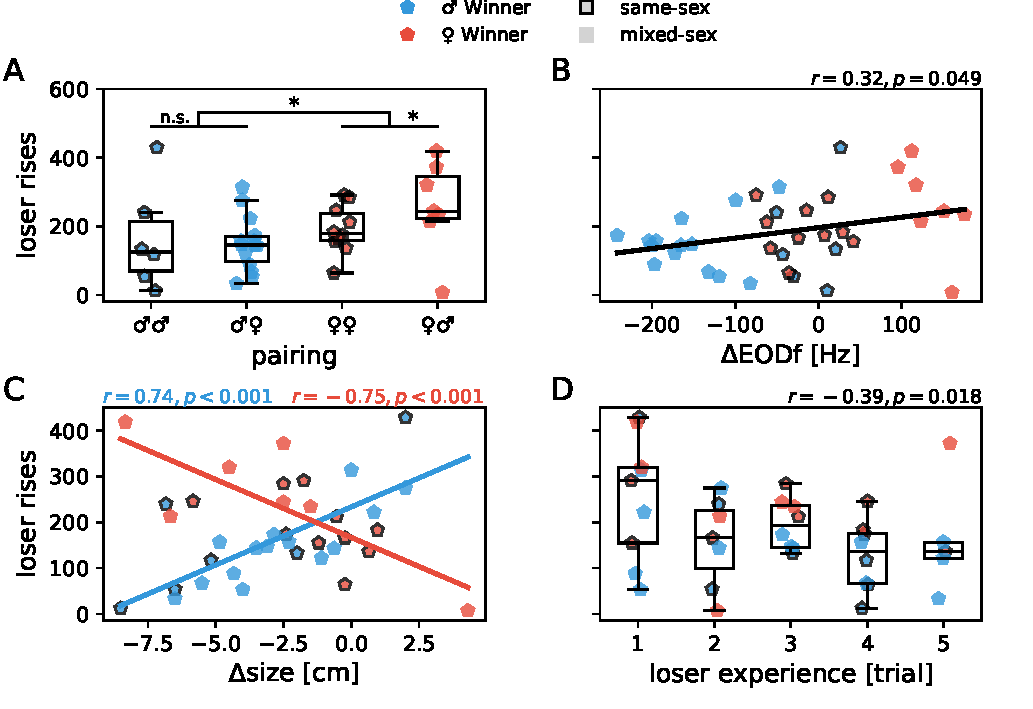
\includegraphics[scale=0.75]{Fig4RiseDependencies}}
  \caption{\label{risefactors} Dependence of rise counts of losing fish on physical differences between competitors and experience. \figitem{A} In trials won by females (red), losers emit slightly more rises than in trials won by males (blue). The first symbol in pairing categories indicates the winner's sex. \figitem{B} With increasing EODf difference to the winning fish ($\Delta\text{EODf} = \text{EODf}_{\text{loser}} - \text{EODf}_{\text{winner}}$), losing fish produced more rises. This effect rests on losing males emitting on average more rises than losing females in mixed-sex competitions (\panel{A}) and males having higher EODfs than females. \figitem{C} In trials won by males (blue), the smaller the size difference to the winner ($\Delta\text{size} = \text{size}_{\text{loser}} - \text{size}_{\text{winner}}$), the more rises were produced by the losing opponent of either sex. In trials won by females (red), the opposite effect was observed. This effect can, however, also result from overall higher rise rates and larger size differences of males compared with females when losing against females (\panel{A}). Correlation coefficients and their significance are displayed in corresponding colors. \figitem{D} With increasing experience in the experiments, losing fish produced fewer rises per trial. * $p \leq 0.05$; n.s. not significant.}
\end{figure}

In trials won by males, the losing competitor of either sex produced less rises than in trials won by females ($U=84.0$, $p=0.02$; \Subfigrefb{risefactors}{A}). Consequently, the number of rises produced by losing fish correlated positively with the difference in EODfs, because of the sexually dimorphic EODf in \lepto{} ($r=0.32$, $p=0.049$; \Subfigrefb{risefactors}{B}). Interestingly, in trials won by males the sex of the losing fish did not have an effect ($U=37.0$, $p=0.36$), whereas in trials won by females losing males produced more rises than losing females ($U=10.0$, $p=0.036$).

\subsection{Sex-specific dependence of rise emission on body size}
The dependence on sex of the winner was even stronger when considering the contestants' body size. In pairings won by males, the number of rises emitted by losers tended to increase with loser size ($r=0.42$, $p=0.064$) and decrease with winner size ($r=-0.51$, $p=0.022$). When regarding the difference in body size, the number of rises emitted by losers increased with its size approaching and exceeding the size of the winning male ($r=0.74$, $p<0.001$, \Subfigrefb{risefactors}{C}). Backward elimination in a multiple linear regression model of number of rises in dependence on absolute sizes of competitors and their difference resulted in size difference as the only parameter ($t=4.72$, $p<0.001$) remaining in the significant model ($F_{1,18}=22.3$, $p<0.001$) with $R^2=0.55$.

In pairings won by females, the number of rises emitted by losers decreased with loser size ($r=-0.55$, $p=0.023$) and was unaffected by winner size. When regarding the difference in body size, the number of detected loser rises decreased the more similar the competitors were in size ($r=-0.75$, $p<0.001$, \Subfigrefb{risefactors}{C}), i.e. the effect was opposite to the one found for trials won by males. In a multiple linear regression model for trials won by females, size difference was the only parameter ($t=-4.36$, $p=0.001$) remaining in the significant model ($F_{1,15}=18.98$, $p<0.001$) with $R^2 = 0.56$ after backward elimination.

\subsection{Habituation of rise rates and loser effects}
The number of rises produced by losers was independent from the outcome of preceding competitions, rejecting a loser effect on the communication behavior of \lepto{}. However, the fish's total experience in the experiment influenced the number of emitted
rises. With increasing experience, i.e. the more trials a fish participated in, the quantity of detected loser rises decreased ($r=-0.39$, $p=0.018$) independently of the paired sexes (\Subfigrefb{risefactors}{D}). The time scale of this habituation matches the one reported for habituation of chirp emission in response to 60\,s long stimulations with an EOD mimic \citep{Harvey2010}.

\subsection{Agonistic interactions}

\begin{figure}[tp]
  \centerline{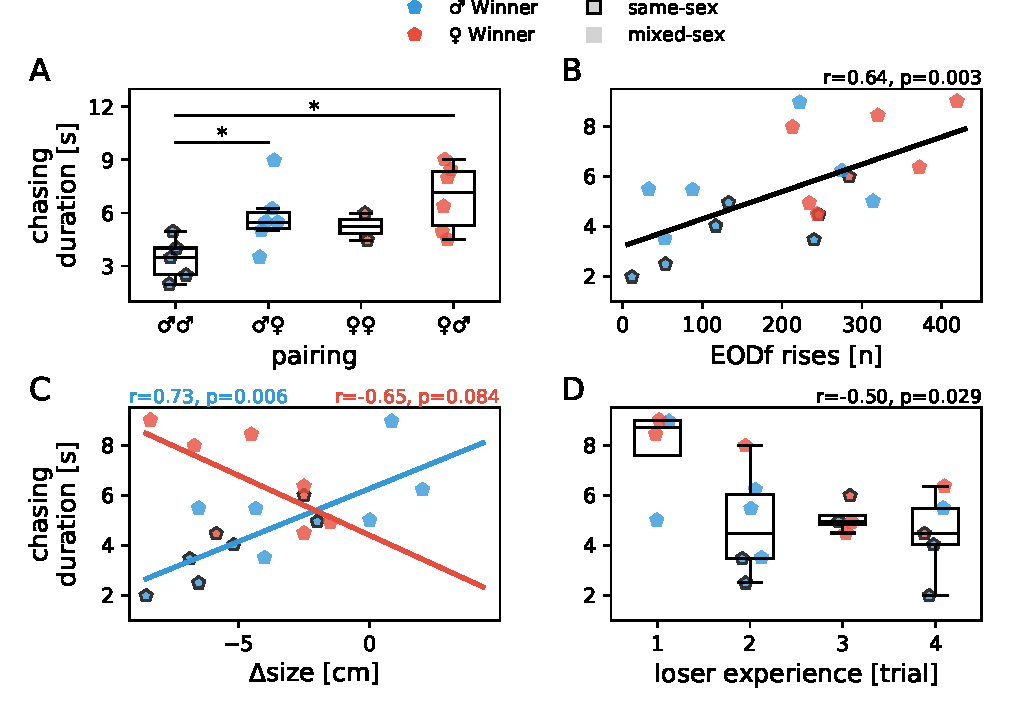
\includegraphics[scale=0.75]{Fig5ChasingDependencies}}
  \caption{\label{agonistics} Agonistic interactions. While the number of agonistic interactions was independent of the physical characteristics of the opponents, the duration of chasing events showed similar dependencies as the number of rises. \figitem{A} The median chase duration was the shortest in male--male interactions. In the annotations of the sex pairings, the first symbol indicates the winner. \figitem{B} The median chase duration increased with the number of rises emitted by losers. \figitem{C} In trials won by males the median chase duration increased with losers approaching and exceeding the size of winners ($\Delta\text{size} = \text{size}_{\text{loser}} - \text{size}_{\text{winner}}$). In trials won by females, the opposite effect was observed; however, similar explanations as for the quantity of rises in the respective pairings apply (\Subfigrefb{risefactors}{C}). Correlation coefficients and their significance are shown in corresponding colors. \figitem{D} With increasing experience in the experiments, the median chase duration decreased. * $p \leq 0.05$.}
\end{figure}

We detected in total 2480 chasing events and 804 agonistic interactions involving physical contact in the 19 trials where we recorded and evaluated these behaviors with IR video. Agonistic interactions were exclusively detected during the dark phase of each trial and stopped with or shortly after the onset of the light phase (\Subfigrefb{trial}{E}). In random visual inspections of video recordings we found that agonistic behaviors were always initiated by those fish later identified as winners. Per trial, we observed on average $128\pm 72$ chase behaviors lasting $7.4\pm 6.5$\,s and $36\pm 21$ physical contacts. The number of physical contacts tended to increase with the number of chasing events ($r=0.37$, $p=0.12$). Interestingly, none of the factors discussed so far had an impact on the number of agonistic interactions, including the competitor's sex, size and EODf differences, and their experience in the experiment. In particular, and similarly to the rises, the number of interactions per trial were highly variable (contacts: $CV=0.55$, chase events: $CV=0.58$) and neither the number of contacts ($r=-0.27$, $p=0.24$) nor the number of chase events ($r=0.30$, $p=0.20$) correlated with the number of rises.

\subsection{Sex-specific dependence of the duration of chase behaviors on body size differences}

The duration of the chase behaviors was sensitive to differences in body size. The median duration of chasing event was shorter in male--male competitions compared with other pairings ($U=5$, $p=0.003$). For other pairings, the median durations of chasing events were indistinguishable (\Subfigref{agonistics}{A}).

In trials won by males, the median chase duration tended to decrease with winner size ($r=-0.58$, $p=0.06$) and was unaffected by size of the losing fish. However, it increased with the size of the losing fish relative to the size of the winner ($r=0.73$, $p=0.006$, \Subfigrefb{agonistics}{C}). Size difference remained after backward elimination the only parameter ($t=3.54$, $p=0.006$) in a linear regression model predicting median chasing duration ($F_{1,9}=12.5$, $p=0.006$) with $R^2 = 0.58$. In trials won by females, median chase duration was independent of absolute sizes but tended to decrease with decreasing size difference between competitors ($r=-0.65$, $p=0.08$, \Subfigrefb{agonistics}{C}). Size difference was the last parameter excluded by backward elimination, but was not significant ($t=-2.07$, $p=0.084$, $R^2=0.42$). Chase durations were not correlated with differences in EODf between the competitors ($r=0.18$, $p=0.45$).

\subsection{Habituation of the duration of chase behaviors}

Beyond physical differences, the experience of the competitors in the experiment influenced the duration of chase behaviors. The duration of chase events decreased with the number of trials the losing fish participated in ($r=-0.50$, $p=0.029$, \Subfigrefb{agonistics}{D}). The number of chase behaviors was unaffected by experience ($r=0.05$, $p=0.83$). Finally, the observed communication behavior had an impact on the chasing duration. In trials where losers emitted more rises, chasing events lasted longer ($r=0.64$, $p=0.003$, \Subfigrefb{agonistics}{B}).

\subsection{Some rises triggered agonistic interactions}
 
\begin{figure}[tp]
  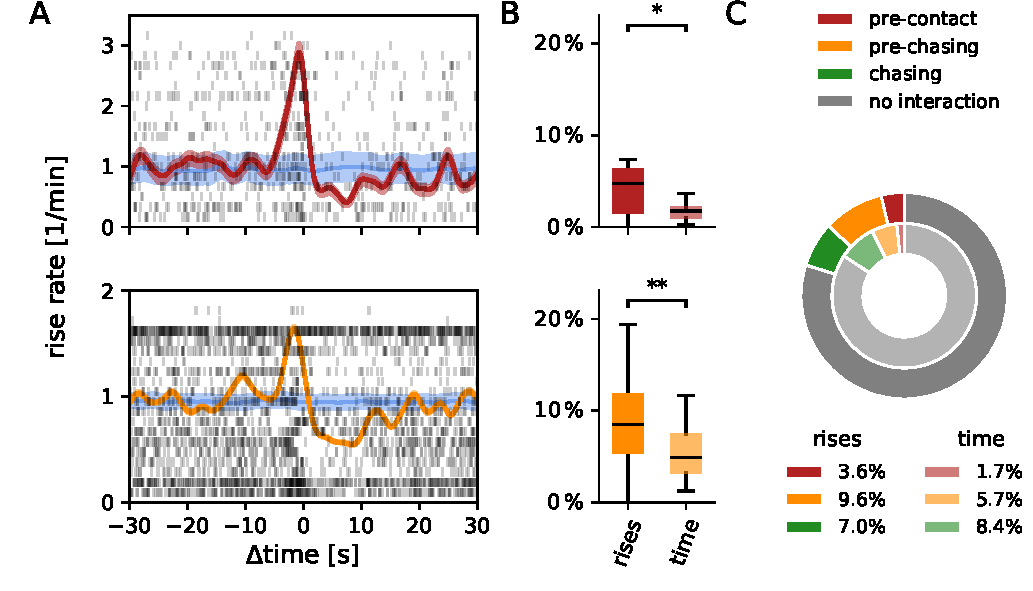
\includegraphics[scale=0.75]{Fig6EventRises}
  \caption{\label{event_rises} Rises trigger other fish to initiate agonistic attacks. \figitem{A} Rise times and rates relative to physical contacts (top) and the onset of chasing events (bottom). Each line of the raster (black) shows rise times aligned to all agonistic events of a single competition trial. Corresponding rise rates (red/orange) were obtained by convolving rise times with Gaussian kernels with s.d. of 1\,s and normalizing by the number of agonistic events and trials. 98\,\% confidence intervals (pink/pale orange areas) were estimated by jack-knifing. The null hypothesis (mean in blue, 1st and 99th percentile in pale blue) was obtained by randomly permuting rise intervals. \figitem{B} Fraction of all rises within the dark phase of a trial that occurred within 5\,s prior to agonistic contacts (top) or the onset of chase behaviors (bottom) and the corresponding times these 5\,s windows make up relative to
the total dark-phase lasting 3\,h. \figitem{C} Mean fractions of rises (outer circle) occurring within 5\,s prior to physical contacts (red), prior to the onset of chase behaviors (orange) and during chase events (green) and the corresponding times (inner circle) over all trials. * $p \leq 0.05$.; ** $p \leq 0.05$.}
\end{figure}

Within $\sim$5\,s prior to agonistic interactions, rise rates accumulated over all agonistic interactions were increased (\Subfigref{event_rises}{A, B}). Because the baseline rate of rises was just one rise per minute, this does not imply that a burst of rises triggered agonistic interactions. Rather, the probability of a single rise to evoke an agonistic interaction was increased. In particular, chances for agonistic contacts were higher 0.7\,s after a rise and chances for chase behaviors were higher 1.6\,s after a rise. Consequently, the fraction of rises occurring within 5\,s before agonistic onset exceeded the fraction expected from the corresponding times, the number of agonistic interactions times 5\,s (agonistic contacts: 3.6\,\% vs 1.7\,\%, $t=2.9$, $p=0.010$; chase behaviors: 9.6\,\% vs 5.7\,\%, $t=-3.1$, $p=0.007$, \Subfigrefb{event_rises}{B}).

\subsection{Reduced rise rates during chase events}

Rise rates were approximately halved during chase events (\Subfigrefb{event_rises}{A}, bottom). After the onset of chasing, the rise rate was reduced for $\sim$10\,s, clearly outlasting the average duration of chase behaviors (7.4\,s). Again, this just implies that the chances of observing a single rise during chasing is reduced. Approximately 7.0\,\% of rises occurred during chase events, less than expected from the corresponding time covered by the chase events (8.4\,\%, $t=3.4$, $p=0.003$, \Subfigrefb{event_rises}{C}).

\subsection{Most rises did not trigger agonistic interactions}
All the rises emitted within 5\,s prior to agonistic contacts and chase events, as well as during the chase events, make up 20\,\% of all rises (\Subfigrefb{event_rises}{C}). Although this is disproportionately more than expected from the corresponding times, the majority of the rises (80\,\%) could not be linked to any obvious interaction. Also, note that the fish engaged in actual agonistic interactions in the form of chase behaviors just 8.4\,\% of the time. Vice versa, agonistic interactions were not exclusively triggered by rises emitted by losers. Rises preceded 15.6\,\% of all chase events and 19.4\,\% of physical contacts,
respectively.

\section{Discussion} % 2350 words

In staged competition experiments between pairs of the electric fish \lepto{} of either sex, we recorded electrocommunication signals, so-called ``rises'', and agonistic behaviors. Losers were characterized by relatively smaller body sizes and their continuously
higher rise emission rates. Rises were costly for losers since they raised the chance of being attacked and being chased for longer by winners. Our results suggest that rises signal an individual's motivation to continue opponent assessment by stimulating ritualized fighting behaviors.

\subsection{Body size as a proxy for RHP in \lepto{}}

An animal's ability to win fights, its RHP, is often correlated to body size or weight, because physical strength is usually directly related to size \citep{Parker1974, Archer1988}. Difference in body size was also the best predictor for the outcome of competitions in our experiments (\Figsrefb{bodysize}, \fref{glm}). Thus, competitors seem to be capable of assessing each other's body size, even in darkness. Electric field amplitudes have been shown to correlate with body size across electric fish species (\eig{}: \citealp{Westby1981}; \sterno{}: \citealp{Hopkins1972}; \albi{}: \citealp{Knudsen1975}). The lateral line organ might provide further sensory cues to assess a contestant's body size \citep{Butler2015}. 

The outcome of competitions can also be influenced by sex-dependent differences in motivation \citep{EnquistLeimar1987, ArnottElwood2008, Dunham2008}. In males, an increased motivation and likelihood to compete has often been observed \citep{Archer1988}. In our experiments, males won competitions slightly more often than females, but mainly because of a bias of males being larger than females in these trials (\Figrefb{bodysize}). Overall, average body size was independent of sex (\Subfigrefb{fishsetup}{A}). However, when evaluated separately, the correlation between body size and winning was more pronounced in trials won by males than trials won by females (\Subfigrefb{bodysize}{B -- E}). This could reflect a higher valuation of suitable shelters by males.

\subsection{Relevant signals and interactions of \lepto{} during competition}
Competitors assess their own and/or their opponent's RHP based on cues, including actively emitted signals, and adapt their behavior accordingly \citep{Cluttonbrock1979, Enquist1990, Payne1998, ArnottElwood2009}. Properties of the continuously emitted electric field of \lepto{}, in particular EODf, could be utilized in opponent assessment. Males increase both EODf and the androgen 11-ketotestosterone at the transition to the breeding season \citep{Cuddy2012} and males with higher EODf seem to fertilize more eggs \citep{Hagedorn1985, Henninger2018}. 

Outside the breeding season, males with higher EODf have been found to be more territorial during the day \citep{Raab2019} and to occupy their preferred shelter alone \citep{Dunlap2002}. Whereas in the latter study EODf was weakly but significantly correlated with body size, we did not have such a correlation (\Subfigrefb{fishsetup}{A}). Consequently, in our experiments, the predictive power of EODf on competition outcome was insignificant (\Figrefb{eodf}), demonstrating only a minor role for EODf signaling RHP in addition to body size.

The RHP of contestants usually affects their fighting behavior, e.g. quantity, intensity, duration or point of giving up \citep{ArnottElwood2009, Taylor2001, Briffa2004}. While in \lepto{} the number of agonistic interactions did not correlate with any of the measured parameters, the duration of chase events was dependent on the difference in contestant's body size, the main factor determining RHP, and the winner's sex (discussed below). Interestingly, the number of rises emitted by losers was correlated in similar ways to the contestant's RHP. This similarity, together with the observation of rises frequently triggering agonistic attacks, suggests that rises play a role in assessing opponents.

\subsection{Electrocommunication with rises}

\lepto{} has been shown to use a rich repertoire of electrocommunication signals in social interactions \citep{Smith2013, Benda2020}. Some of the various types of chirps, transient elevations of EODf within less than $\sim$500\,ms, are used in agonistic same-sex encounters to deter agonistic attacks \citep{Hupe2008, Henninger2018} and in courtship, where synchronization of spawning is probably only one of their many functions \citep{Hagedorn1985, Triefenbach2003, Cuddy2012, Henninger2018}. In contrast, evidence for the function of rises is scarce and inconsistent. Rises are characterized by smaller but much longer increases in EODf in comparison to chirps \citep{Hopkins1974, Hagedorn1985}. They vary considerably in their size (a few up to several tens of Hertz) and over three orders of magnitude in their duration (less than a second to up to a few minutes, \citealp{Tallarovic2002}). The large number of rises we detected in our experiments clearly formed a continuous distribution of sizes and durations, and we found no indication of distinct functional roles of rises of different sizes \citep{Triefenbach2008}, refuting earlier attempts to categorize rises \citep{Hagedorn1985, Tallarovic2002,Dye1987}.

\subsection{Function of rises}

Rises have been observed to be followed by attacks or bouts of aggression, both in \textit{Eigenmannia} \citep{Hopkins1974} and \lepto{} \citep{Triefenbach2008}, and to primarily be emitted by subordinates in \Albi{} \citep{Serrano2003}. We also found rises in \lepto{} to be primarily emitted by losing fish (\Subfigrefb{EODfriserates}{A, B}) and agonistic interactions to be more frequent after the emission of rises (\Subfigref{event_rises}{A}). These common findings further support the hypothesis of rises being conserved signals in gymnotiform electric fish \citep{Turner2007}.

As only $\sim$20\,\% of rises were followed by agonistic interactions, one could argue that rises are submissive signals aiming to avert upcoming agonistic attacks. However, the emission of more rises did not decrease the number of agonistic interactions and even increased the duration of chasing events (\Subfigrefb{agonistics}{B}), suggesting that rises rather encourage agonistic interactions than deter them. This contradicts the interpretation of rises as submissive signals \citep{Hopkins1974,Serrano2003} and as a general expression of stress \citep{Smith2013}. Chirps, in contrast, have been shown to reduce attack probability in competition experiments \citep{Hupe2008}. \lepto{} thus use a variety of electrocommunication signals of different meanings in social interactions.

Communication signals in general aim to alter the behavior of a receiver in a net beneficial fashion for the sender and they are only produced when the potential benefits outweigh the costs \citep{Endler1993, Seyfarth2010}. In contests, they can convey information about physical condition and RHP \citep{Davies1978, Cluttonbrock1979}, social status \citep{Huyghe2005, Fernald2014}, and motivation or behavioral intent (e.g. aggression: \citealp{Triefenbach2008, Kareklas2019}; or submission: \citealp{Hupe2008, Silva2012}) and often already convey sufficient information to settle competitions without the necessity of escalating costly fights \citep{ArnottElwood2009}. In our experiments, winners could reliably be predicted within the initial 25\,min of each trial based on the number of rises emitted by either fish (\Subfigrefb{EODfriserates}{C}). Nevertheless, losers continued to emit more rises than the winner until the end of the dark phase (\Subfigrefb{EODfriserates}{D}). We never observed a switch in communication behavior between contestants (\Subfigrefb{EODfriserates}{E}). Therefore, rises were apparently not used to ultimately win competitions. What then is the purpose of rises?

\subsection{Sexual dimorphic behavioral traits}

Male \lepto{} have been shown to be more territorial than females \citep{Dunlap2002} and show more intense dominance displays \citep{Raab2019}. Females, in contrast, are
more tolerant to the presence of conspecifics \citep{ZupancMaler1993, Cuddy2012}. All these observations could be explained by an increased resource valuation in males (territoriality at shelters) in comparison to females, and males being more motivated to win
competitions. Our data further support this hypothesis, as discussed below.

In trials won by males, both the number of rises and the duration of chase events increased with decreasing size difference between contestants (\Subfigsrefb{risefactors}{C}, \subfref{agonistics}{C}). This is not unusual, because of increased chances of success when competing with opponents of similar size (e.g. \citealp{Cluttonbrock1979, Enquist1990}). A higher motivation of males could be inferred by losers by means of behavioral cues and interpreted as potentially higher costs when engaging in competition, which could reduce a loser's motivation to compete. This could explain the overall lower rise production by losers in trials won by males (\Subfigref{risefactors}{A}) and the resulting shorter chase events (\Subfigref{agonistics}{A}).

In trials won by females, we found the opposite relationship. With decreasing size difference fewer rises were produced by the losing fish and chase duration decreased (\Subfigsrefb{risefactors}{C}, \subfref{agonistics}{C}). These negative correlations, however, are mainly carried by the sex of the losing fish. Males losing against females tended to be much smaller (\Subfigref{bodysize}{E}) and at the same time emit more rises (\Subfigref{risefactors}{A}) and interact longer during chase events (\Subfigref{agonistics}{A}) compared with all other pairings. Females competing against females were more similar in size (\Subfigsrefb{bodysize}{C}, \subfref{fishsetup}{A}), emitted fewer rises (\Subfigref{risefactors}{A}) and had shorter chase events (\Subfigref{agonistics}{A}). The higher intrinsic motivation of males in addition to the lower potential costs in competing with less territorial females could explain the enhanced rise production in males regardless of RHP of female opponents.

In other species, the mere presence of a potential mating partner often affects communication (e.g. \citealp{Barske2015}) and other behaviors associated with reproductive success \citep{Taylor1975}. Accordingly, the specific sex pairing could evoke males to emit
disproportionately more rises when losing against females. Males could additionally be motivated to continue assessment in order to indicate increased fighting capabilities and appear more suitable as potential mating partner. However, winning males not emitting
more rises towards females and females responding with equal levels of aggression to rises of both sexes (\Figref{agonistics}) rather argues against rises to signal a male's quality to females in our competition experiments.

Nevertheless, competition between \lepto{} and associated behaviors presumably change with reproductive state. The motivation of males to compete could be enhanced, especially for same-sex rivals. Females could use male rises to assess their capability and motivation to compete and thus their quality. Testing these speculations, however, requires extensive breeding experiments.

In summary, the dependence of rise production on the fish's RHP and the link between agonistic interactions and rise emission support our hypothesis of rises signaling an individual's motivation to continue opponent assessment using ritualized fighting. The fact
that both behaviors are also dependent on the competitor's sex additionally suggests sexually dimorphic behavioral traits in \lepto{}, potentially arising from a higher motivation of males to win competitions despite substantial differences in RHP.

\subsection{Mutual assessment in \lepto{}}

Analyzing the dependence of competition behaviors on the contestants' RHP allows to differentiate between assessment strategies, i.e. pure self-, cumulative or mutual assessment \citep{ArnottElwood2009}. In cumulative assessment, costs arising from an individual's own actions during competitions and those being inflicted by opponents are accumulated until an endurance threshold is reached and the animal retreats \citep{Payne1998}. In our experiments, however, this threshold never seems to be reached, because rise emission and agonistic interactions went on throughout the dark phase. For pure self-assessment, a positive correlation between both contestants' absolute RHP and the extent of behaviors associated with competition is expected \citep{Taylor2001}. This can be rejected, because absolute body size of neither winner nor loser predicted competition outcome (\Subfigref{bodysize}{F}), and both the number of rises and duration of chasing events rather decreased with winner size.

Both, communication and agonistic behaviors remained steady throughout single trials. Both are presumably low-cost behaviors, because no injuries or other negative consequences resulted from them. This supports mutual assessment where low-cost competition behaviors are repetitively performed in order to accurately assess an opponent's RHP relative to their own (e.g. \citealp{Cluttonbrock1979}). Furthermore, animals are expected to improve in accuracy of assessing the opponent with increasing experience \citep{Enquist1990, Grosenick2007}. This matches previous observations on decreasing competition intensity over trials in another gymnotiform electric fish \citep{Westby1970} as well as our own observations on \lepto{} where the number of emitted rises and the duration of chasing events decrease with the fish's experience in the competition experiment (\Subfigsrefb{risefactors}{D}, \subfref{agonistics}{D}).

\subsection{Dominance in \lepto{}}

Competitions are not exclusively used to directly secure access to resources, but also to establish dominance hierarchies, that indirectly regulate access to resources \citep{Wauters1992, Sapolsky2005, Taves2009}. After establishing dominance, knowledge about an individual's social status can prevent costly repetitive fighting and therefore can be beneficial for all individuals involved \citep{Fernald2014, Huyghe2005}. Characteristics of social hierarchies and behavioral correlates of dominance vary widely across species \citep{Cluttonbrock1979, Cigliano1993, Sapolsky2005}. In group living species, beyond regulating access to resources, social hierarchies often occur with complex social dynamics, such as leader-follower dynamics (e.g. \citealp{Strandburg2018, Jason1990}). In solitary species, in contrast, dominance is primarily associated with resource-based benefits \citep{Cigliano1993}.

Dominance hierarchies have also been suggested for \lepto{} \citep{Hagedorn1985, Dunlap2002}. Since behavioral observations suggest that \lepto{} is a solitary living species \citep{Stamper2010, Raab2019, Henninger2020}, this dominance can be assumed to be mainly resource based.

Previous studies suggest that male but not female \lepto{} form a dominance hierarchy \citep{Hagedorn1985, Dunlap2002}. Indeed, as discussed above, males seemed to be more motivated to win competitions. Nevertheless, competition outcome was independent of the contestant's sex and mainly determined by relative body size (\Figrefb{glm}). Dominance in \lepto{} thus appears to be sex-independent, in line with similar studies on other gymnotiform electric fish \citep{Silva2012, Zubizarreta2020}.

\subsubsection{Rises in the social hierarchy of \lepto{}}

In social hierarchies, dominants often use agonistic attacks to keep subordinates under control \citep{Cluttonbrock1979, Creel1996, Janson1985}. In \lepto{}, subordinates could emit rises to signal their motivation to continue assessment, with the aim to reduce relative dominance (e.g. \citealp{Kareklas2019}). Dominants, in contrast, could counteract with agonistic attacks. The interplay and balance between rises and agonistic attacks could define the relative dominance between contestants and regulate skewness in access to resources. This would imply that motivation of the fish in the competition depends on the valuation of not only present but also regularly encountered resources, most likely food, that were absent during our experiments.

This hypothesis on a possible benefit of continuous rise emission by losers is supported by a single exceptional trial, where the dominant fish shared the superior shelter with the subordinate at the end of a trial. In this mixed-sex trial, the smaller male (11.9\,cm) was
continuously emitting 180 rises during the dark phase and apparently succeeded in reducing the relative dominance difference to the larger female (12.5\,cm, no rises during dark
phase) by gaining access to the shelter.


\subsection{Conclusion}

Male \lepto{} seem to be more motivated to win staged competitions for a superior shelter than females. Nevertheless, contest outcomes were mainly determined by relative body size, reflecting the contestants' overall fighting ability, their RHP. During competition, \lepto{} interact physically by means of ritualized fights and use rises as distinct electrocommunication signals. The extent of both behaviors depends on the contestants'
RHP, suggesting that \lepto{} assess their opponents during contests (mutual assessment). Here, rises are almost exclusively emitted by losers and seem to signal their motivation to continue physical assessment. Rises triggered agonistic attacks and enhanced
the duration of chase events. The motivation to continue assessment could reflect a loser's attempt to reduce relative dominance, which is counteracted by dominant fish with agonistic attacks.

%%%%%%%%%%%%%%%%%%%%%%%%%%%%%%%%%%%%%%%%%%%%%%%%%%%%%%%%%%%%%%%%%%%%%%%%%%%%%%%%

%
%%%%%%%%%%%%%%%%%%%%%%%%%%%%%%%%%%%%%%%%%%%%%%%%%%%%%%%%%%%%%%%%%%%%%%%%%%%%
%\section{Acknowledgements}
%Supported by Deutsche Forschungsgemeinschaft via mini RTG ``Sensory
%flow processing across modalities'' by the excellence cluster ``Center
%of Integrative Neuroscience'' (CIN EXC 307).
%% Open Access Publishing Fund of University of T\"ubingen.
%
%%\begin{contributions}
%%  T.R. designed the experiment, measured and analyzed data, and wrote the manuscript. S.B. and S.E. measured the data. J.B. discussed the experiment, advised data analysis, and edited the manuscript.
%%\end{contributions}

%\bibliographystyle{jneurosci}
%\bibliography{../journalsabbrv,../references}

\newpage
\section{Supplementals}

\renewcommand\thefigure{S\thechapter.\arabic{figure}}
\setcounter{figure}{0}   

\begin{figure}[!h]
  \centerline{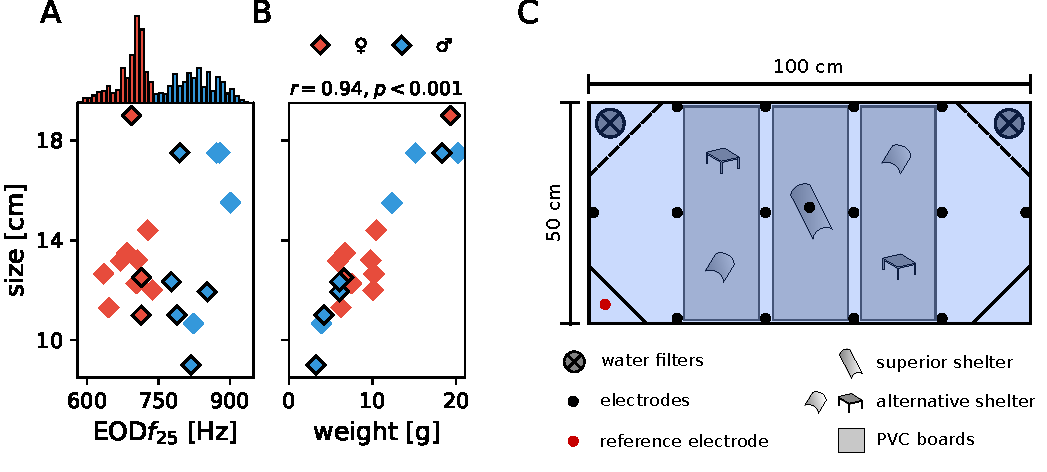
\includegraphics[scale=0.75]{FigS1FishSetup}}
  \caption{\label{fishsetup} Physical characteristics of the fish and experimental setup. \figitem{A} EODf and size (length) of each of the 21 \lepto{} participating in the experiments. EODf was not correlated with size, neither for all fish nor within the sexes. EODfs were temperature corrected to 25\,\celsius. Males (blue) were identified by their higher EODfs compared to female EODfs (red). The histogram on top shows the distribution of EODfs of either sex measured in all trials for every five minutes. Black marker edges indicate fish whose sex has been verified by gonadal inspection. \figitem{B} Weight and size of fish were independent of sex and increase proportional to each other. \figitem{C} The competition tank was equipped with one high quality shelter (center tube) and four low quality shelters (two short tubes and two tables) attached to PVC-boards. A total of 15 electrodes (black circles) were distributed in the tank to record electric behaviors of interacting fish. Two air-powered water-filters were placed in the corners behind PVC boards with netted windows (dashed lines). The other two corners were shielded with PVC boards (black lines), one of them contained the reference electrode (red circle).}
\end{figure}

\begin{figure}[t]
  \begin{minipage}[t]{0.5\textwidth}\mbox{}\\[-2ex]  
    \centerline{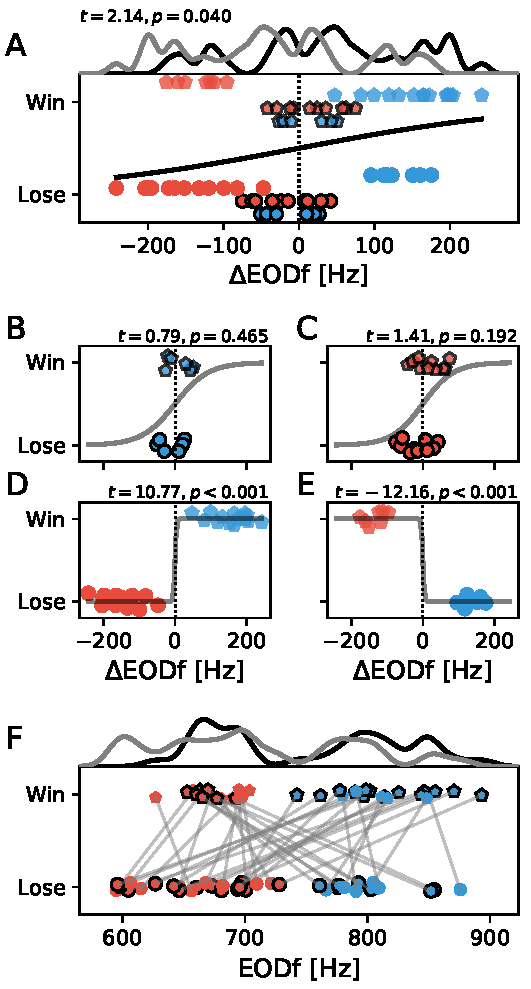
\includegraphics[scale=0.75]{FigS2EODf}}
  \end{minipage}
  \hfill
  \begin{minipage}[t]{0.45\textwidth}
  \caption{\label{eodf} EOD frequencies of winners and losers. Same annotation scheme as in \Figref{bodysize}. \figitem{A} Winners tend to have higher EODfs than their opponents. \figitem{B, C} Winners of same-sex encounters do not have significantly higher EODfs than losers ($\text{AUC=73}$\,\%). \figitem{D, E} In mixed-sex competitions the sexual dimorphic EODf does not predict competition outcome. More males ($n=14$) were winning mixed-sex trials than females ($n=7$), explaining the overall trend of winners having higher EODfs than losers (panel~\panel{A}). \figitem{F} Absolute EODf of winners and losers convey even less information about the outcome of the competitions ($\text{AUC=65}$\,\%).}
  \end{minipage}
\end{figure}

\begin{figure}[!h]
  \centerline{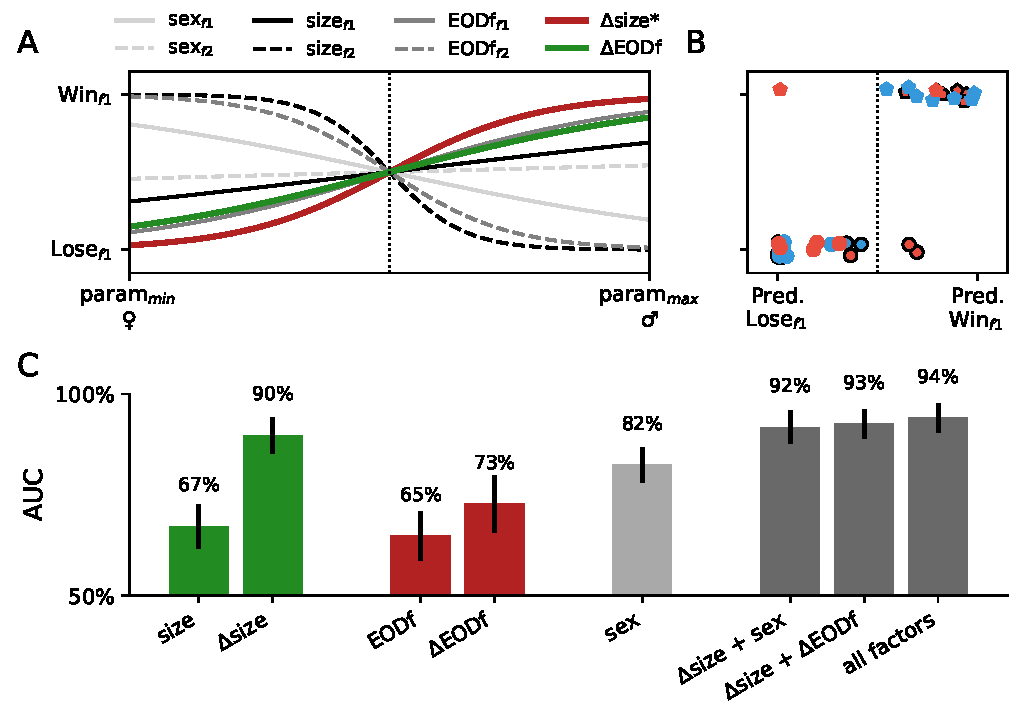
\includegraphics[scale=0.75]{FigS3GLM}}
  \caption{\label{glm} Logistic regression models predicting the outcome of competitions. \figitem{A} Visual representation of the impact of all factors (sex, absolute size, and EODf of fish $f1$ and $f2$, as well as their differences in size and EODf) on the generalized linear model with a logistic link function, corresponding to table~\ref{glm_table}. The steeper the logistic functions the more discriminative the respective factor. Size difference, $\Delta$size, is the only significant factor. \figitem{B} Predictions of the GLM on fish$_1$ of each of the 37 competition trials being the winner or loser based on all factors shown in \panel{A}. Same marker code as in \Figref{bodysize}. \figitem{C} Area under the curve (AUC, with standard deviation estimated by bootstrapping) extracted from a receiver-operating-characteristic (ROC) analysis to quantify the performance of single factors and combinations of factors to discriminate winners of competitions from losers. Chance level is at $\text{AUC} = 50$\,\%.}
\end{figure}

\renewcommand\thefigure{\thechapter.\arabic{figure}}
\setcounter{figure}{0}   
%\figurecaptions

\cleardoublepage
\graphicspath{{chapter_5_discussion/}}
% crossref 
%\externaldocument{../chapter_2_methods/chapter_methods}
%\externaldocument{../chapter_3_habitats/chapter_habitats}
%\externaldocument{../chapter_4_competition/chapter_competition}


\chapter{Discussion}

The work I am presenting in this thesis was largely inspired by the natural behavior of \lepto{} we observed during a field trip to Colombia in 2016 in the context of my master thesis. Since to this time, field studies on electric fish were rare and the development of precise hypotheses was accordingly complicated, we simply recorded the electric signals of present fish continuously for a period of two weeks using a grid of 64 electrodes. Back in the lab, we developed and tested different hypotheses while analyzing the recorded data. The on-site experiments of our field trip, including recordings with simple handheld devices, i.e. transect recordings, suggested \lepto{} to coexist in high densities in the wild. Accordingly, we expected to observe a multitude of behaviors that can be associated with the social life of these fish. However, when we started to analyze the data, we were overwhelmed by the large number of recorded fish and the complexity of their behaviors. We detected up to 26 fish in about 3.5\,m$^3$, exceeding our expectations by magnitudes and significantly complicating reliable signal tracking. The applied algorithms only provided rather fragmentary EODf traces with many flawed connections and therefore required extensive manual corrections (\figref{Colombia_traces}). Nevertheless, I was able to gain preliminary insights into the fish's natural spatio-temporal and even electrocommunication behavior.

\begin{figure}[h!]
  \centerline{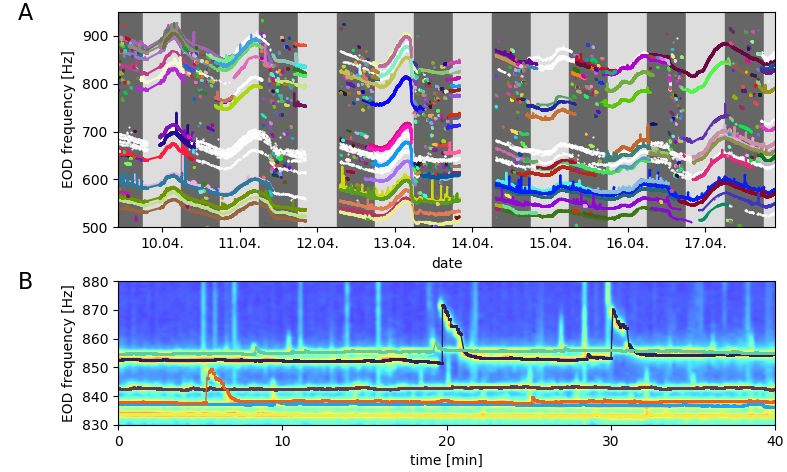
\includegraphics[width=1\textwidth]{traces}}
  \caption{\label{Colombia_traces} Long-term field recording of \macros{}, a member of the \lepto{} species group, in Colombia, 2016. EODs were recorded with a 64 channel electrode array covering $3.5 \times 3.5$\,\meter\squared. \figitem{A} Eight days of EODfs detected and tracked. Each reliably detected fish is indicated in a different color. Unreliable detections for which we need to further improve our algorithms are indicated in white. Dark gray areas indicate night time, light gray areas day time. \figitem{B} Spectrogram of a 40 minute long section of the recording from April 14$^{th}$, 2016 with tracked EODf traces. EODf traces frequently cross each other when fish emit rises as electrocommunication signals.}
\end{figure}

The tracking issues that arose from the complexity of electric recordings obtained in the wild encouraged me to improve tracking algorithms in cooperation with Noah Cohen's Lab at the Johns Hopkins University in Baltimore, USA (\chapref{Methods}). These improvements were crucial for evaluating the complex electric long-term recordings obtained in subsequent experiments (and in the wild) since they reduced the expense of extensive EODf trace post-processing. Furthermore, the behavioral complexity we observed in the wild clearly indicated the necessity for elaborate laboratory experiments to first gain understanding of the different aspects of the natural social life of \lepto{}, including the causalities of associated behaviors, before being able to make sense of the complex behavioral data contained in field recordings. 


%Furthermore, the behavioral complexity we observed in the wild clearly indicated the necessity for elaborate laboratory experiments in order to understand the different aspects of the natural social life of \lepto{}, including the causalities of associated behaviors, and then be able to make sense of the complex behavioral data contained in field recordings. 
%
%Furthermore, the behavioral complexity we observed in the wild clearly indicated the necessity for elaborate laboratory experiments. In order to make sense of the complex behavioral data contained in such recordings, we first need to gain understanding of the different aspects of the natural social life of \lepto{}, including the causalities of associated behaviors.

Consequently, my thesis pursued two main objectives: (i) The development of an algorithm capable of tracking individual EODs in various electrode array settings and (ii) the utilization of this technique in different behavioral experiments aiming to advance our knowledge about the different aspects of the social life of \lepto{} and the causalities of associated behaviors. Ultimately, these objectives aimed towards better understanding of its behaviors observed and recorded in the wild that, without knowledge gained from laboratory studies, would remain difficult to interpret.

In \chapref{Methods}, a semi-automatic system capable of tracking individual EODs based on individual-specific EOD features is presented. The algorithm combines previous approaches of tracking either the individual-specific EODf \citep{Henninger2020} or the spatial properties of an individual's electric field \citep{Madhav2018}. Furthermore, it has been inspired by the general approach of biometric systems, i.e. detecting specific manifestations of an animal's behavior or appearance (biometric entities) in order to classify them according to predefined biometric profiles, which correspond to typical manifestations of these biometrics in, for example, a certain species, individual, or behavior \citep{Gaston2004, Sherley2010,  Kuhl2013}. These advancements considerably increased tracking accuracy and reduced the effort of post-processing tracked EOD traces. Accordingly, the algorithm facilitates the evaluation of complex multi-electrode recordings, enabling large-scale studies on freely moving and interacting electric fish populations, even in high densities. 

The development of this advanced tracking algorithm was a requirement for the experiments described in \chapref{Habitats}~\&~\ref{Competitions}. Utilizing these techniques, we were able to monitor and characterize individual spatial-temporal behaviors within a group of 14 \lepto{} over 10 consecutive days (\chapref{Habitats}, \citealp{Raab2019}). In this experiment, fish have been housed in a large communal tank (2m$^3$ water capacity), stocked with several naturalistic habitats inspired by their natural environment observed in Colombia (\subfigref{eodtraces}{A, B}). The evaluated movement patterns suggest fish to mainly distribute independently from each other according to the presence of suitable shelters (\subfigsref{eodtraces}{E}, \subfref{habitatpref}{C}). Interestingly, individual diurnal activity patterns correlated with EODf. In male \lepto{}, higher EODf has previously often been associated with dominance \citep{Hagedorn1985, Dunlap2002, Triefenbach2008}. In our study, males with higher EODf showed enhanced explorative behavior during the night and increased territoriality during the day (\subfigref{transitions}{B}), which both could represent manifestations or displays of dominance. Females, on the other hand, have previously been suggested to form no dominance hierarchy at all \citep{Hagedorn1985} or only a less pronounced one, causing females with higher EODf to be more likely found inside of shelter-tubes \citep{Dunlap2002}. In our study, we found females with higher EODf to be more active during both day and night (\subfigref{transitions}{B}), suggesting EODf in females to indicate more active character traits rather than dominance. 

In a subsequent study, we evaluated behaviors and interactions of unfamiliar pairs of \lepto{} during staged competitions (\chapref{Competitions}, \citealp{Raab2021}). Fish with larger body size usually won competitions, i.e. occupied the superior shelter during the light phase at the end of the trial (\figref{bodysize}). EODf and sex played a secondary role at best (Table~\ref{glm_table}). During the dark phase of each trial, fish showed typical competition behaviors in terms of ritualized fighting supplemented by electrocommunication with rises (\figref{trial}). Rises were almost exclusively emitted by losers (\subfigref{EODfriserates}{A, B}), whereas agonistic interactions were exclusively initiated by winners. The number of rises emitted by losers and the duration of chase behaviors depended in similar ways on the contestants' physical attributes. Detailed evaluations of these correlations suggest \lepto{} to adjust their competition behavior according to mutual assessment \citep{EnquistLeimar1987} and males to presumably be more motivated to win competitions \citep{ArnottElwood2008}. Rises seemed to be costly in terms of increasing the probability to trigger winners into initiating agonistic actions and to be chased for a longer time period (\figref{event_rises}). Regardless, losers continued to emit rises even after the winner of a trial was, according to a clear difference in communication behavior, already determined (\subfigref{EODfriserates}{C, D}). Since both rise quantity and average duration of agonistic interactions increased with decreasing difference between the contestants' RHP (\subfigsref{risefactors}{C}, \subfref{agonistics}{C}), i.e. according to mutual assessment, we suggest rises to signal a loser's motivation to continue assessment, ultimately aiming to reduce relative dominance and alter the skewness in general access to resources in its favor \citep{Sapolsky2005}. Interestingly, males who lost against females seemed to be additionally motivated to continue assessment. In the respective trials, males emitted rises at high rates despite of large RHP differences to the winning females (\subfigref{risefactors}{A, C}).

Our studies demonstrate the capability of the developed algorithm to track electric signals of individual electric fish, including electrocommunication signals, even in complex long-term grid recordings (\chapref{Methods}). This technique enabled us to obtain a plethora of unadulterated behavioral data on freely moving and interacting \lepto{}. By evaluating the observed behaviors in the context of common competition and dominance theories, we have advanced our knowledge about the secretive social life of \lepto{} and set the stage for the success of future behavioral studies on the natural behavior of electric fish, including the analysis of complex recordings made in the wild. 

\section{Implications for data processing}

The technological advances of the last decades greatly increased our capabilities to study natural and undisturbed animal behaviors across various species \citep{Hughey2018, Jolles2021}. A common technique to monitor animals and their behaviors in their natural habitats is the utilization of bio-loggers, i.e. small animal mounted devices, equipped with different sensors (e.g. \citealp{Strandburg2015}). An alternative approach is to detect animals and their behaviors in external recordings, e.g. obtained with remote sensing devices like drones equipped with different sensors, or directed stationary camera-, microphone-, or electrode-setups \citep{Anderson2014, Dell2014, Hughey2018}. Each technique, however, comes with different challenges for data processing and handling. For example, external recording devices provide rather unspecific data that requires extensive processing in order to obtain reliable and exploitable behavioral data (e.g. \citealp{Kuhl2013, Dell2014}).

Likewise, our approach of recording electric signals of freely moving electric fish using arrays of recording electrodes provided rather unspecific data, too. In order to derived distinct behavioral traces for individual fish from our data, we pursued and adapted the approach of an animal biometric system \citep{Kuhl2013}. Commonly, this approach involves pattern detection and classification by means of machine-learning or deep-learning algorithms. Specific animal biometrics, i.e. manifestations of an animal's behavior or appearance, are classified by comparing them to predefined biometric profiles, i.e. typical manifestations of a respective tracking category, like species, identity, or a certain behavior \citep{Burghardt2006, Sherley2010, Ernst2011}. However, this method only provides reliable results with static biometric profiles that show little to no overlap in their definite characteristics. 

Being restricted to EOD characteristics, biometric profiles corresponding to individual electric fish are rather unspecific. Spatial electric field properties change with a fish's movement \citep{Madhav2018} and its EODf in the context of communication \citep{Zupanc2002, Triefenbach2008, Smith2013}. This variability results in potentially overlapping EOD features between individuals that consequently can lead to tracking errors. Nevertheless, each of these EOD features itself have formed the basis of one of the previous tracking approaches \citep{Madhav2018, Henninger2020}. Since both approaches track signals consecutively according to their temporal detection, their tracking accuracy further decreases for data sections where signals of single fish are temporarily not detected (e.g. detection losses caused by too large distances to recording electrodes). Both approaches achieve high tracking accuracy when evaluating low density fish populations. However, with increasing abundance and accordingly increasing overlap of individual EOD features (smaller EODf differences and similar locations of multiple fish), tracking issues accumulate and accuracy decreases respectively.

To circumvent these issues, we partly detach the tracking process from the temporal detection of signals. Instead of tracking signals in the order of their temporal detection, we identify potential signal pairs in 30\,second tracking windows and link them in a succession of decreasing signal similarity (\figref{tmp_tracking}). Consequently, we not only avoid tracking errors caused by temporal signal detection losses, but also ensure signal traces to be generated according to the highest similarity between signal pairs. Additionally, our algorithm benefits from utilizing a combined signal error comprising both EODf and spatial field property difference for tracking individual EOD traces. Rapid changes in one of these signal features, e.g. caused by rapid movements or the emission of a communication signal, can be compensated by the respective other signal feature, whereby tracking errors can be avoided.

Despite our advancements in tracking accuracy, sporadic manual corrections of flawed EODf traces remain necessary. In its current state, the presented algorithm establishes new signal pair connections solely based on their similarities. Indeed, even better tracking results could be achieved by implementing signal trace predictions that dynamically adapt to already established connections within a current tracking segment. Corresponding implementations, however, would require an even more dynamic tracking algorithm and multiply the required computational power and time beyond efficient scientific feasibility. In future studies, a neural network could be trained on tracking individual EODf traces, similar to existing pose detection algorithms (e.g. \citealp{Mathis2018}). Such approaches, however,  require extensive training data-sets in order to perform with reliable accuracy. Accordingly, our algorithms and evaluated data-sets might represent the basis for the development of such an even more advanced tracking system in the future.

In conclusion, our developed algorithm not only improves tracking accuracy of wave-type electric fish compared to previous approaches \citep{Madhav2018, Henninger2020}, but also advances the general approach of biometric systems \citep{Kuhl2013}. By refraining from static biometric profiles and rigid classifications in favor of probabilistic time-variant classifications, we enhanced the general applicability of this method. Our method relies only on the extraction of specific features suitable for describing a tracking category in external recordings. In our case, this corresponds to EOD features extracted from electrode grid recordings and used for tracking electric signals of individual fish. However, since these tracking features can be anything detectable in external recordings of any modality, our method is not limited to tracking electric fish alone, but can also be adapted to tracking tasks across various animal species, or even beyond behavioral studies or science in general. 

A major benefit of machine-aided analysis is its capability to process enormous amounts of data (mainly automatically). This is not only useful to solidify specific scientific statements \citep{Gomez2014, Dell2014}, but also enables important explorative studies. In our case, machine-aided analysis was crucial to enable our explorative recordings of populations of \lepto{} in their natural habitats in Colombia. Even though at the time, we were unable to understand the specific significance and causalities of observed behaviors, these field trips led to specific hypotheses and the development of the laboratory experiments described in \chapref{Habitats} and \ref{Competitions} and further discussed below. 

\section{Implications for the social life of \lepto{}}

Behavior does not occur in a contextual vacuum \citep{Rendall1999, Seyfarth2017, Henninger2018}. Accordingly, in order to understand the meaning and causalities of specific behavioral events, a detailed understanding of the framework in which behaviors occur is vital (e.g. \citealp{Rendall1999, Henninger2018}). A crucial aspect shaping the scope of possible interpretations of social behaviors is the structure and organization of an animal's social environment. For example, specific communication signals in group living species can frequently be associated with behavioral coordination or cooperation (e.g. group cohesion, \citealp{Demartsev2018}, collective anti-predator defense \citealp{Schibler2007}; reconciliation, \citealp{Cheney1995}, etc.). However, for solitary species, a coherence between communication and mate attraction or agonistic actions is way more likely, simply because of their respective way of life \citep{Cornhill2020}. 

The social organization of \lepto{} has rarely been addressed in previous studies. For other electric fish species, primarily those belonging to the family of African \textit{Mormyrides}, different behavioral patterns have been identified suggesting them to be live in social groups. Some electric fish species form shoals (e.g. \textit{Mormyrus rume proboscirostris}, \citealp{Worm2021}, \textit{Mormyrops anguilloides}, \citealp{Arnegard2005}, or \Eigenmannia, \citealp{Oestreich2005}), emit communication signals that can be associated with group cohesion \citep{Arnegard2005, Worm2021}, and even forage or hunt collectively in a group \citep{Arnegard2005, Bastos2021}. 

For \lepto{}, corresponding observations are sparse. In the laboratory, \lepto{} distribute independent from each other according to the availability of suitable shelters (\subfigref{eodtraces}{E}, \subfref{habitatpref}{C}). Similar observations have also been made in the field (own observations in Colombia, 2016, 2019, \citealp{Stamper2010}). On the other hand, in a forced choice experiment \citet{Stamper2010} observed \lepto{} to reliably approach tubes with EOD mimics of con-specifics instead of non-stimuli tubes. However, considering that \lepto{} shows increased aggression towards con-specifics compared to other electric fish species (e.g. \citealp{Triefenbach2008}), this approaching behavior is presumably rather associated with initial assessment and competition than with the intention of shoaling. 

Nevertheless, Gymnotiform fishes, including \lepto{}, make up to 70\,\% of the biomass of large rivers in South America \citep{Marrero1991, Cox2004, Crampton2011}. Therefore, frequent interactions with con-specifics are inevitable. We ourselves observed high densities of \lepto{} in a small river in Colombia (up to 26 individuals in about 15\,m$^2$, \subfigref{Colombia_traces}{A}). However, neither ourselves nor other studies observed or reported individual behaviors as evidence for \lepto{} to be a group living species, e.g. collective movement or cooperation. Therefore, we suggest \lepto{} to actually be a rather solitary living species that is forced to share its habitat with con-specifics because of their high abundance. Yet individual fish could benefit passively from the presence of con-specifics, e.g. by means of an overall reduced individual predation risk or increased reproductive success \citep{Cote1995, Clutton-Brock1999, Sword2005, Bilde2007}. On the other hand, fish also have to face the challenges arising from increased intra-specific rivalry for limited resources (e.g. \citealp{Janson1985, Chapman1995, Markham2017}). The diversity of social interactions in \lepto{} we observed and evaluated in the process of this thesis could have been developed in order to facilitate the frequent social encounters and interactions that inevitably result from their high abundance in natural habitats.

%\subsubsection{Behavioral interactions in \lepto{}}
\subsection{Assessment during competitions in \lepto{}}

\begin{figure}[h!]
  \centerline{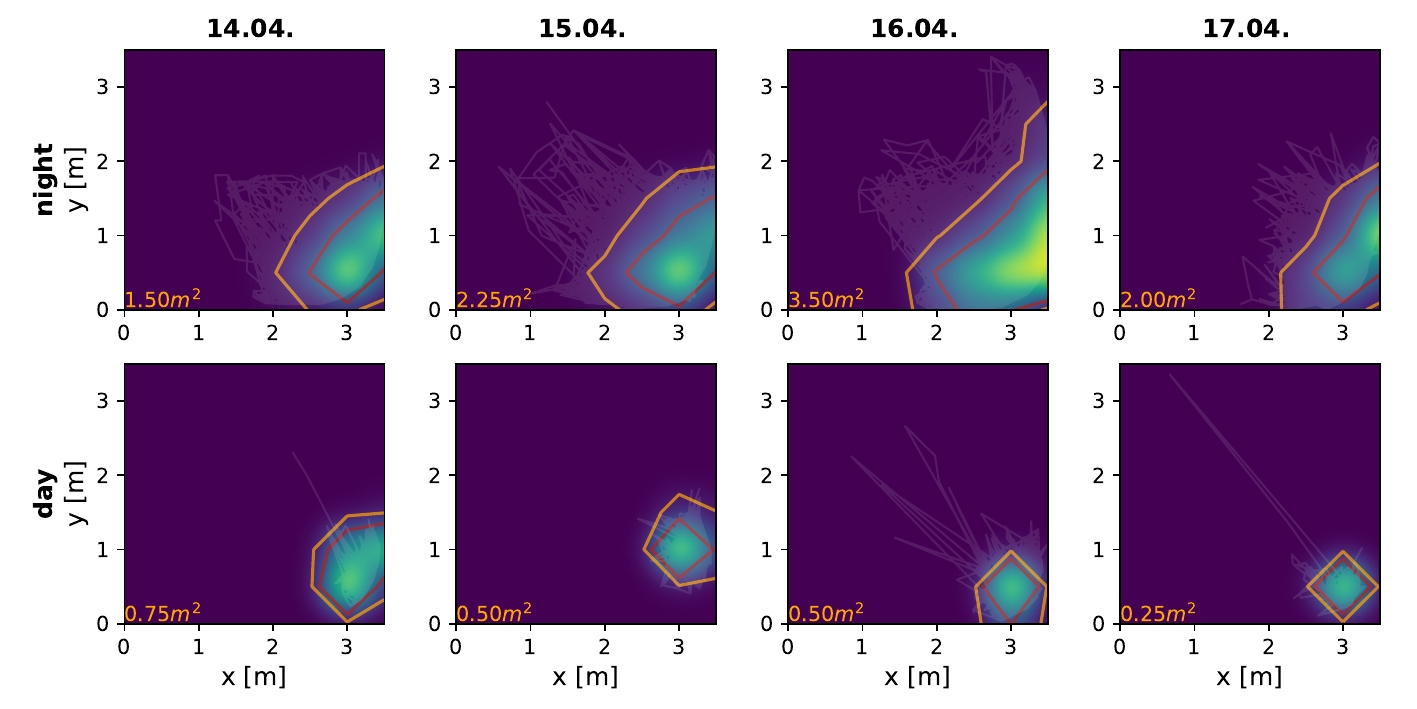
\includegraphics[width=1\textwidth]{stationary_jpg}}
  \caption{\label{Colombia_stationarity} Spatial behavior of a single \macros{} detected and tracked consecutively for four days. Heat-maps and contour lines show the fish's probability of presence across the monitored 3.5$\times$3.5\,m$^2$ area of the river during the night (top panels) and day (bottom panels). Orange contour lines include the area in which the fish spends more than 50\,\% of the time, the red lines more than 75\,\% of the time respectively. Even though the fish certainly shows movement behaviors, especially during the night, it remains remarkably stationary in the bottom-right corner of the observation area for four consecutive days.}
\end{figure}

In the presence of con-specifics, animals frequently rival for limited resources and fighting is usually a key behavior to secure access \citep{Cluttonbrock1979, Chapman1995, Markham2015}. However, competition is costly in terms of time and energy allocated to it and an increased risk of injury or death (e.g. \citealp{Briffa2004}). In order for competitions to be evolutionary stable, potential benefits always need to outweigh the associated costs \citep{ArnottElwood2009}. Accordingly, different species developed various mechanisms to economize competitions, e.g. specific assessment strategies \citep{EnquistLeimar1987, Payne1998, Taylor2003} or a dominance hierarchy to regulate access to resources (e.g. \citealp{Janson1985, Sapolsky2005}). Which mechanism eventually manifests in a given species, depends on its social organization and given environmental situations. The development of a complex dominance hierarchy is most beneficial if repetitive rivalry with the same individuals is likely. Developing elaborated assessment strategies can be useful when animals frequently compete with the same as well as different individuals. When competitions are rather scarce or resources are abundant, presumably neither of these mechanisms will develop because the costs of developing associated behaviors are not covered by the resulting benefits.

In order to understand how \lepto{} resolves conflicts, we evaluated their competition behavior during staged competitions (\chapref{Competitions}, \citealp{Raab2021}). Competitions were usually won by the larger individual, suggesting resource holding potential (RHP, \citealp{Parker1974}) in \lepto{}, i.e. an individual's potential to inflict and endure damage \citep{Archer1988}, to be primarily based on body size. In our experiments, additional factors influencing the outcome of competitions, like positional advantages, were intentionally eliminated by the experimental design. However, in the fish's natural habitats, where we observed highly stationary fish (Colombia, 2016, \figref{Colombia_stationarity}), positional advantages of a resident could still bias competitions to be rather won by residents than intruders, as observed in other species (e.g. \citealp{Alcock1997}). 

In some species, animals actively assess their individual chances of winning competitions by interpreting passive cues and active signals which indicate their opponent's fighting motivation and capability \citep{Cluttonbrock1979, EnquistLeimar1987}. This information exchange can often already be sufficient to resolve conflicts without the necessity of costly escalating physical fighting \citep{Parker1974, Cluttonbrock1979, Jason1990}. In \lepto{}, observed competitions comprised ritualized fighting \citep{Triefenbach2008} accompanied by rises as electrocommunication signals \citep{Smith2013}. Agonistic events were initiated by the winners of trials whereas rises were primarily emitted by the respective losers. Both behaviors occurred with unvarying frequency within trials, and their extent similarly increased with decreasing size difference between competitors. This suggests (i) behavioral decision making in competitions between pairs of \lepto{} to be based on mutual assessment and (ii) both ritualized fighting events and rises to be important in terms of information gathering during this process. These conclusions, again, match with our observations made in the fish's natural habitats. As aforementioned, \lepto{} can be found in high densities in the wild. However, at the same time we only found little food items in the corresponding clear streams. With many fish to compete over sparse high value resources, the development of behaviors associated with mutual assessment is reasonable and the most economic approach to resolve the corresponding conflicts \citep{ArnottElwood2009}.

\subsubsection{Electrocommunication with rises}

Our competition experiment suggests rises to be emitted by losers in order to signal their motivation to continue assessment. Thus, during competitions, rises can be assumed to be an important signal to gain valid information about a con-specific in the process of mutual assessment. Accordingly, their emission should be net beneficial and evolutionary stable, even though they are costly in terms of increasing chances of being attacked or chased for a longer time period (\figref{event_rises}). However, rises are rather generic signals. They show huge variations in terms of duration (lasting from seconds up to many minutes) and EODf increase (up to 68\,Hz). In some configurations, rises can potentially even be confused with other active EODf modulations observed in \lepto{}, e.g. a short jamming-avoidance response \citep{Tallarovic2005}. The structural variability of rises indicates that they are rather unspecific signals with little informative value \citep{Seyfarth2003}. We suggest the specific meaning of rises to arise from the behavioral context they are emitted in \citep{Seyfarth2003}. During competitions, rises seem to signal motivation \citep{Raab2021}. Further applications of rises in various behavioral contexts could potentially be revealed in detailed observations of whole populations of \lepto{} under more naturalistic conditions.

\subsection{Implications on the social hierarchy in \lepto{}}

Even though elaborate assessment strategies can economize competitions \citep{ArnottElwood2009}, costs still accumulate when animals rival with the same individuals over and over again. To further economize these rivalries, some species fight in order to establish dominance hierarchies, where an animal's access to resources is determined by its social status (e.g. \citealp{Wauters1992, Sapolsky2005, Taves2009}) and mutual knowledge about hierarchical ranks prevents repetitive fights among familiar individuals \citep{Cluttonbrock1979, Fernald2014, Cornhill2020}.

Dominance hierarchies have also been suggested for various electric fish species \citep{Westby1970, Fugere2011, Silva2012}, including \lepto{} \citep{Hagedorn1985, Dunlap2002, Stamper2010, Henninger2018}. Previous studies suggest that male but not female \lepto{} form a dominance hierarchy \citep{Hagedorn1985, Dunlap2002}. More dominant males have been reported to occupy higher quality shelters, preferably alone \citep{Dunlap2002}, and to show increased participation in reproduction \citep{Hagedorn1985, Henninger2018}. Females, on the other hand, have been suggested to either form no dominance hierarchy at all \citep{Hagedorn1985}, or only a distinct one, whereby less dominant females are more likely to be found outside of shelter tubes \citep{Dunlap2002}. 

As discussed above, we suggest \lepto{} to actually prefer remaining solitary over living in groups, even though they are forced to share their natural habitats with con-specifics because of their high abundance. Dominance in \lepto{} can therefore be assumed to be rather resource based, as in other solitary species (e.g. \citealp{Cigliano1993}), instead of coming along with complex social structures and group behaviors, like, for example, the development of a leader-follower dynamic \citep{Strandburg2018}. Accordingly, determining whether the social life of \lepto{} is shaped by a social hierarchy or repetitive competitions over resources is complicated in experiments with short observation times, but can potentially be answered by interpreting individual behaviors in long-term observations. 

As aforementioned, we found \lepto{} in abundance in the wild where individuals frequently remained rather stationary over several days (\figsref{Colombia_traces},\fref{Colombia_stationarity}). Accordingly, frequent interactions and rivalry with the same individuals are inevitable and the development of a dominance hierarchy would be the most efficient way to distribute resources and reduce the necessity of repetitive costly fights \citep{Sapolsky2005}. Further support for the social life of \lepto{} being shaped by a dominance hierarchy instead of fighting in repetitive competitions arises from their observed communication behavior. Rises have only occasionally been observed in the wild and their quantity seemed to decrease throughout the two weeks of our first laboratory experiment (\subfigref{eodtraces}{C}). Since we could further show that rises are reliably emitted in the context of competition between pairs of \lepto{} \citep{Raab2021}, this suggests competitions to be rather sparse in the wild and to decrease over time in artificially compound populations. Consequently, rises and competitions can be assumed to be mainly used to establish dominance during initial encounters, which then regulates access to resources and prevents the high costs of repetitive fighting.

\subsubsection{Skewness of the social hierarchy in \lepto{}}

In our competition experiments, dominance is attained through agonistic interactions and resources are claimed entirely by dominants. At first glance, this suggests a despotic dominance hierarchy for \lepto{} \citep{Kappeler2008}. On the other hand, these agonistic interactions resemble non-escalating ritualized fights \citep{Triefenbach2008} which are often used to intimidate con-specifics and obtain or maintain dominance in rather egalitarian hierarchies across species \citep{Sapolsky2005}. Furthermore, we did not observe active displacement from micro-habitats in our first group experiment, indicating fish to tolerate the presence of con-specifics and, consequently, to share available resources. We suggest our contradictory observation of fish monopolizing resources in our competition experiments to result from the very limited resources in this experiment that could hardly be shared anyway. Further support for more egalitarian dominance hierarchies in \lepto{} comes from their observed communication behavior during staged competitions. Losers continued to emit rises at a constant rate and thereby stimulated agonistic attacks, even though the outcome of competitions was presumably already set and mutually recognized within the initial phase of interactions. However, continued mutual assessment could be used to adjust relative dominance between competitors and thereby the skewness in access to resources, which can be assumed to be obsolete in despotic hierarchies. Finally, our hypothesis of a rather egalitarian hierarchy in \lepto{} is further supported by the preliminary observation of multiple males participating in reproduction in the wild \citep{Henninger2018}. 

\subsubsection{EODf as signal of dominance}

In order for dominance hierarchies to economically resolve conflicts between con-specifics, individuals need to be able to assess each other's social status. Accordingly, different species developed specific signals conveying corresponding information \citep{Cluttonbrock1979, Fernald2014, Cornhill2020}. When fish are not in each other's direct proximity, \lepto{} can exclusively exchange information with con-specifics using their EODs \citep{Knudsen1975, Henninger2018, Henninger2020, Benda2020}. Therefore, these electric signals would be most suitable to signal dominance in \lepto{}. Indeed, some studies found dominance to correlate with EODf in males, and to some extend also in females \citep{Hagedorn1985, Dunlap2002, Triefenbach2008}. Furthermore, in males EODf has sometimes been found to correlate with body size \citep{Dunlap2002, Triefenbach2008}. 

In our competition experiments we did not find a correlation between body size and EODf in either sex. Nevertheless, the accuracy of our generalized linear model predicting winners of competitions increased slightly when including EODf as an additional parameter besides body size (\figref{glm}). Furthermore, we clearly found EODf dependent spatio-temporal movement traits for both sexes in our first laboratory experiment, which, at least for males, can also be associated with dominance or corresponding displays (\subfigref{transitions}{B, D}). Both our own observations as well as the inconsistency across studies in finding a link between EODf and body size or dominance suggest EODf to be, at best, an unreliable predictor for dominance. Nevertheless, as aforementioned, the EODs of electric fish are the only source of information that can be accessed by con-specifics from afar. Accordingly, EODf could be used as an initial rough estimate of a potential opponent's body size, RHP, or dominance. 

As discussed above, we suggest rather egalitarian dominance hierarchies for populations of \lepto{}. In this kind of social organization, the evolutionary pressure to compete with con-specifics can be expected to be reduced in comparison to despotic hierarchies. Accordingly, validating the rough dominance estimate obtained from a potential competitor's EODf by approaching them and risking physical competition could be too costly to outweigh the potential benefits. \lepto{} could therefore rely on EODf as a signal of dominance when the availability of resources is generally sufficient and fish mainly perceive each other electrically, e.g. in our first open space laboratory experiment or in the wild.

\section{Sexually dimorphic behavioral traits}

In our experiments, we repeatedly found sexually dimorphic behavioral traits. For males, we could identify distinct movement behaviors that can be associated with dominance or interpreted as corresponding displays, i.e. territoriality at shelters during the day and increased exploration behavior during the night (\subfigref{transitions}{B, D}). Furthermore, the correlation between larger body size and winning staged competitions was stronger in males compared to females (\subfigref{bodysize}{B--E}) and males emitted an especially high number of rises when losing against larger females (\subfigref{risefactors}{A, C}). Together with previous observations of males showing increased territoriality \citep{Dunlap2002} and increased overall aggression towards con-specifics compared to females, this suggests a generally boosted motivation in males to win competitions and gain or maintain dominance. These motivational differences could explain the observed behavioral divergences between males and females \citep{ArnottElwood2008}.

% boosted motivation in males
In our experiment, we could not clearly determine the cause for the suggested motivational differences between the sexes and the resulting sexually dimorphic behavioral traits. However, since access to different limited resources, e.g. food, shelter, etc. is usually  determined by an animal's social status \citep{Janson1985, Blumstein2001, Charpentier2005, Dunham2008}, we suggest a sexually dimorphic valuation of these resources to be a possible cause for the respectively observed behavioral differences in \lepto{}. 

Although \lepto{} is sexually quite monomorphic, which suggests requirements for food or shelter and their valuation to be rather similar for both sexes, a possible divergence could arise from \lepto{} mating behavior. During the mating season, males are known to compete for females, which after an extensive mating ritual spawn a single egg in a location save from external threats such as strong currents or predators. Under the assumption that females assess the quality of a male by assessing the suitability of its shelter for reproduction, shelters could be some kind of secondary sexual characteristic of males and therefore increase their motivation to compete for them. Nevertheless, it should be noted that in \rostratus, a close relative of \lepto{}, preliminary observations suggest males to visit females in the context of mating, rather than \textit{vice versa}, which contradicts our hypothesis.  


% dominance in females 

\subsection{Females in the dominance hierarchy of \lepto{}}

As discussed above, the observed behavioral traits of females in our experiments suggest them to be less eager to prevail in social contexts. Contrary to males, we did not find movement behaviors that can be associated with dominance or corresponding displays and body size was less predictive for winning competitions. These observations are consistent with previous studies suggesting females to be overall less aggressive and more tolerant towards the presence of con-specifics compared to males (e.g. \citealp{Dunlap2002}). Accordingly, the only competition trial in which we observed both contestants sharing the superior shelter in the end was won by a female (the other contestant was male; loser identified by rise quantity). Altogether, the more peaceful and passive behavioral characteristics suggested for females could, indeed, be associated with them not forming a dominance hierarchy as suggested in previous studies \citep{Hagedorn1985, Dunlap2002}. 

On the other hand, fish of both sexes showed similar (even though not identical) competition behaviors during our staged competitions. Another possible yet still rather hypothetical and uninvestigated explanation could be that females are evolutionary less reliant on dominance and associated benefits. The rather egalitarian dominance hierarchy previously suggested for \lepto{} in this thesis, could generally provide sufficient resources for females and limit their active participation in dominance fights to occasions where resources are scarce, e.g. in our competition experiments.

\section{Open ends and perspectives}

In the presented thesis, I demonstrate how extensive behavioral observations in an animal's natural environment can lead to specific scientific questions and the development of elaborate techniques and complex laboratory experiments in order to answer them. In our case, we developed tools, techniques, and laboratory experiments to advance our knowledge about the behavioral adaptations in \lepto{} which enable them to successfully inhabit their natural habitats in high densities.

% competition
Our results suggest \lepto{} to economize the frequent conflicts inevitably resulting from their high abundance in the wild through mutual assessment. By means of ritualized fighting and information exchange via electrocommunication, contestants gather information about each other's resource holding potential and adapt their behavior according to the disparity. In this process, rises seem to be important signals to coordinate competitions. With their emission, subordinates seem to signal their motivation to continue assessment by stimulating ritualized fighting. In order to further increase our knowledge about the different social aspects of competitions in \lepto{}, we plan to adjust the experimental design of future competition experiments to enable the additional detection and evaluation of chirps. In previous studies, these communication signals have already been associated with agonistic interactions and could therefore reveal further details of the fish's competition behavior when included in our analysis. 

% social organization in \lepto{} - how to verify it ?
The evaluation of individual behavioral traits and social interactions of \lepto{} in the context of this thesis provides a strong basis for developing hypotheses regarding the overall social structure in populations of \lepto{}. Together with our observations from the field, the conclusions of our laboratory experiments indicate \lepto{} to (i) develop dominance hierarchies, where (ii) an individual's access to resources is proportional to its social status, and (iii) males are more motivated than females to gain dominance and associated benefits.

Even though all of our conclusions derive from elaborate and detailed behavioral observations, some assume still unverified causalities and therefore require further scientific validation. Accordingly, future experiments should increase in complexity and gradually approximate natural conditions in order to create experimental setups where these questions can potentially be answered. For example, detailed observation of competitions and associated behaviors in small groups of \lepto{} competing over divisible and measurable resources (e.g. distributed small food items or shelters of varying quality as in \citealp{Dunlap2002}) could help to clarify the skewness in access to resources across the dominance hierarchy in populations of \lepto{}. Furthermore, such elaborate experiments could potentially lead to the discovery of still unrevealed behavioral traits and causalities that only emerge and are observable in more complex social and environmental settings. The ultimate prove for our hypotheses could be obtained by inducing breeding conditions and evaluating individual reproductive success throughout a group of \lepto{}. However, since breeding conditions induce complex changes in an animal's behavior, corresponding experiments should be conducted only after the evaluation of individual behaviors and interactions within smaller groups in complex environments (as suggested above) have been exploited. Breeding experiments could, furthermore, reveal interesting behavioral changes that complement our understanding about the social life of \lepto{}. For example, females could become more active and motivated to win competitions because their valuation of food might increase due to increased energy demand and their valuation of shelters might increase since they correspond to save spawning sites.

% How to get back to the field ? 
As repetitively mentioned throughout this thesis, our work was inspired by the complexity of electric recordings obtained from the fish's natural habitats. With the behavioral observations of our laboratory experiments, we already developed a strong basis for identifying specific behaviors solely based on characteristic electric signal changes and associated spatio-temporal behaviors. For example, we showed that rises frequently trigger agonistic interactions that come along with high velocity movement behaviors. Both electric and spatio-temporal manifestations of behaviors can also be extracted from grid recordings of electric fish in the wild. Accordingly, further laboratory experiments could provide the basis to develop an electro-spatio-temporal ethogram of \lepto{}. Such an ethogram could then be utilized to detect specific behaviors and interactions in the wild and validate their significance and causalities in the environments these behaviors have originally evolved to.  

%\bibliographystyle{jneurosci}
%\bibliography{../journalsabbrv,../references}
%

% FOR CROSS-REF ACROSS CHAPTERS
%https://tex.stackexchange.com/questions/14364/cross-referencing-between-different-files
%
%\bibliographystyle{jneurosci}
%\bibliography{journalsabbrv,references}
\cleardoublepage
\fancyhead[LE]{}
\fancyhead[RO]{Bibliography}
\thispagestyle{plain}
\bibliography{journalsabbrv,references}
\figurecaptions


\end{document}
